% Полезные ссылки:
% * https://habrahabr.ru/post/144648/ - Диплом бакалавра в LaTeX, или ДСТУ 3008-95 в 150 строк
% * http://dkhramov.dp.ua/Comp/NIRReportDSTU300895 - Оформление отчета о НИР в LaTeX
% * http://dkhramov.dp.ua/index.php?n=Comp.CyrillicInListingsTex - Оформление исходного кода в документах LaTeX
% * http://mydebianblog.blogspot.ru/2012/12/latex.html - Как оформить исходный код программ в LaTeX без адских страданий
% * http://aakinshin.blogspot.ru/2014/01/latex-minted.html -  minted: Оформляем исходный код в LaTeX
% * http://s.arboreus.com/2008/12/russian-thesis-in-latex.html - советы: Диссертация в LaTeX

\documentclass[a4paper,14pt]{article}
%\documentclass[a4paper,12pt]{article}

% Русский язык (LaTeX)
%\usepackage[T1,T2A]{fontenc}
%\usepackage[utf8]{inputenc}
%\usepackage[english,russian]{babel}

% Русский язык и шрифты (XeLaTeX)
\usepackage{xunicode}
\usepackage{xltxtra}
\usepackage[english,russian]{babel}
\usepackage{xecyr}
\defaultfontfeatures{Ligatures={TeX}}
\setsansfont[Path=./fonts/arial/, UprightFont=*, ItalicFont=*i, BoldFont=*bd, BoldItalicFont=*bi]{arial}
\setmonofont[Path=./fonts/courier_new/, UprightFont=*, ItalicFont=*i, BoldFont=*bd, BoldItalicFont=*bi, Mapping=]{cour}
\setmainfont[Path=./fonts/times_new_roman/, UprightFont=*, ItalicFont=*i, BoldFont=*bd, BoldItalicFont=*bi]{times}

% Отступ у первого абзаца
\usepackage[indentfirst]{titlesec}

% Возможность сделать 14-й шрифт
\usepackage{extsizes}
\usepackage{anyfontsize}

% Междустрочный интервал
%\linespread{1.35}
\usepackage[nodisplayskipstretch]{setspace}
%\onehalfspacing
\setstretch{1.4}
% Нет интервала между элементами списков
\usepackage{enumitem}
\setlist{nosep}
% Отступы в списках
%\setitemize[0]{leftmargin=0pt, itemindent=35pt}
\setitemize[0]{leftmargin=1.5cm, itemindent=0cm}
\setenumerate[0]{leftmargin=1.5cm, itemindent=0cm}

% Интервал между абзацами
%\setlength{\parskip}{6pt}

% Поля страницы
\usepackage[left=3cm,top=2cm,right=1cm,bottom=2cm]{geometry}

% Отступ для абзаца
\setlength{\parindent}{1cm}

% Литература с точки + нормальные ссылки
\usepackage[square,numbers,sort&compress]{natbib}
\renewcommand{\bibnumfmt}[1]{#1.\hfill}
%\def\@biblabel#1{#1.}

% Нефиг делать гигантские интервалы между элементами списка литературы
\setlength{\bibsep}{0.5ex plus 0.3ex minus 0.2ex}

% Начать нумерацию страниц не с 1
%\setcounter{page}{4}

% Картинки
\usepackage{graphicx}

% Каталог для картинок
\graphicspath{ {./images/} }

% Разные таблицы
\usepackage{tabularx, multirow, tabu}
\newcolumntype{L}[1]{>{\hsize=#1\hsize\raggedright\arraybackslash}X}
\newcolumntype{R}[1]{>{\hsize=#1\hsize\raggedleft\arraybackslash}X}
\newcolumntype{C}[1]{>{\hsize=#1\hsize\centering\arraybackslash}X}
%\newcolumntype{C}[2]{>{\hsize=#1\hsize\columncolor{#2}\centering\arraybackslash}X}

% Алгоритмы
% http://blog.harrix.org/?p=648
\usepackage{algorithm2e}
\SetKwInput{KwData}{Исходные параметры}
\SetKwInput{KwResult}{Результат}
\SetKwInput{KwIn}{Входные данные}
\SetKwInput{KwOut}{Выходные данные}
\SetKwIF{If}{ElseIf}{Else}{если}{тогда}{иначе если}{иначе}{конец условия}
\SetKwFor{While}{до тех пор, пока}{выполнять}{конец цикла}
\SetKw{KwTo}{от}
\SetKw{KwRet}{возвратить}
\SetKw{Return}{возвратить}
\SetKwBlock{Begin}{начало блока}{конец блока}
\SetKwSwitch{Switch}{Case}{Other}{Проверить значение}{и выполнить}{вариант}{в противном случае}{конец варианта}{конец проверки значений}
\SetKwFor{For}{цикл}{выполнять}{конец цикла}
\SetKwFor{ForEach}{для каждого}{выполнять}{конец цикла}
\SetKwRepeat{Repeat}{повторять}{до тех пор, пока}
\SetAlgorithmName{Алгоритм}{алгоритм}{Список алгоритмов}

% Таблицы и рисунки по ГОСТу
\usepackage[tableposition=top, singlelinecheck=false]{caption}
\DeclareCaptionLabelFormat{gostfigure}{Рисунок #2}\DeclareCaptionLabelFormat{gosttable}{Таблица #2}
\DeclareCaptionLabelSeparator{gost}{~---~}
\captionsetup{labelsep=gost}
\captionsetup*[figure]{labelformat=gostfigure, justification=centering}
\captionsetup*[table]{labelformat=gosttable, justification=raggedright}
\usepackage{subfig}
\renewcommand{\thesubfigure}{\asbuk{subfigure}}
% в рисунках: h - "хотелось бы картинку здесь"; h! - "очень хочу картинку здесь"; H - "ХОЧУ картинку здесь и баста", p - на отдельной странице, t - сверху
% Управление плавающими штуковинами (рисунками, таблицами, etc)
\usepackage{float}

% Точки после номеров разделов
\usepackage[subfigure]{tocloft}
\renewcommand{\cftsecaftersnum}{.}
\renewcommand{\cftsubsecaftersnum}{.}
\makeatletter
\def\@seccntformat#1{\csname the#1\endcsname.\ }
\makeatother

% Даешь подсекции в оглавление
\setcounter{tocdepth}{3}

% Размер шрифтов в названиях секций/подсекций
\addto{\captionsrussian}{\renewcommand*{\contentsname}{{\fontsize{14}{16}\selectfont Оглавление}}}
\titleformat{\section}{\normalfont\fontsize{14}{16}\bfseries}{\thesection.}{1ex}{}
\titleformat{\subsection}{\normalfont\fontsize{14}{16}\bfseries\itshape}{\thesubsection.}{1ex}{}
\titleformat{\subsubsection}{\normalfont\fontsize{14}{16}\bfseries\itshape}{\thesubsubsection.}{1ex}{}

% Размер шрифтов в содержании
\renewcommand\cftsecfont{\normalfont}
\renewcommand\cftsecpagefont{\normalfont}

% Точки в секциях
% https://tex.stackexchange.com/questions/53898/how-to-get-lines-with-dots-in-the-table-of-contents-for-sections
\renewcommand{\cftsecleader}{\cftdotfill{\cftdotsep}}

% Запрет висячих строк
\clubpenalty=10000
\widowpenalty=10000

% Для формул
\usepackage{amsmath}
\usepackage{mathtools}
\usepackage{amsfonts}
\usepackage{amssymb}
\usepackage{amsbsy}

% Работа с цветом
% http://habrahabr.ru/post/52166/
\usepackage[usenames,dvipsnames]{color}
\usepackage{colortbl}

% Разные подчеркивания
% https://tex.stackexchange.com/questions/27258/how-do-i-write-underline-text-but-with-a-dotted-line
\usepackage{tikz}
\newcommand{\dotunderline}[1]{%
    \tikz[baseline=(todotted.base)]{
        \node[inner sep=1pt,outer sep=0pt] (todotted) {#1};
        \draw[densely dotted] (todotted.south west) -- (todotted.south east);
    }%
}%

% Раскопировать пробелы
\newcommand\spacedfill[1]{\makebox[#1]{\leaders\hbox{~}\hfill}}

% Отступ для формул
\makeatletter
\g@addto@macro\normalsize{%
  \setlength\abovedisplayskip{20pt}
  \setlength\belowdisplayskip{20pt}
  \setlength\abovedisplayshortskip{5pt}
  \setlength\belowdisplayshortskip{15pt}
}
\makeatother

% Код программы
% http://mydebianblog.blogspot.ru/2012/12/latex.html
\usepackage{verbatim}
\usepackage{minted}

% Структурированный pdf
\usepackage[bookmarksnumbered=true,bookmarksopen=true,breaklinks=true,pdfborder={0 0 0},linktoc=all]{hyperref}

% Удобные ссылки на электронные ресурсы
\usepackage{url}
\renewcommand\UrlFont{}

% Кастомное имя метки
% https://tex.stackexchange.com/questions/73664/how-to-nameref-to-partial-part-of-a-ref
\usepackage{nameref}
\makeatletter
\newcommand{\labelname}[1]{% \labelname{<stuff>}
	\def\@currentlabelname{#1}}%
\makeatother

% Минимальное количество букв, которые можно переносить
\righthyphenmin=2

% Борьба с overfull
\tolerance=300000

% Перенос знаков во внутритекстовых формулах (использовать так $a\hm+b\hm+c\hm+d$)
%\newcommand*{\hm}[1]{#1\nobreak\discretionary{}{\hbox{$\mathsurround=0pt #1$}}{}}
% Можно также просто запретить переносить знаки операций и отношений
\binoppenalty=10000
\relpenalty=10000

%
\title{Отчет по производственной практике}
\author{Жигалов П.С.}

% Счетчики страниц и всякого разного
\usepackage{lastpage, totcount}
% Счетчик рисунков
\newtotcounter{foofigure}
\makeatletter
\renewenvironment{figure}[1][\fps@figure]{
  \edef\@tempa{\noexpand\@float{figure}[#1]}
  \@tempa
  \addtocounter{foofigure}{1}
}{
  \end@float
}
\makeatother
% Счетчик таблиц
\newtotcounter{footable}
\makeatletter
\renewenvironment{table}[1][\fps@table]{
  \edef\@tempa{\noexpand\@float{table}[#1]}
  \@tempa
  \addtocounter{footable}{1}
}{
  \end@float
}
\makeatother
% Счетчик источников в списке литературы
\newtotcounter{foobibitem}
\def\oldbibitem{}
\let\oldbibitem=\bibitem
\def\bibitem{\stepcounter{foobibitem}\oldbibitem}

% Команды и сокращения
\renewcommand{\Re}{\mathop{\mathrm{Re}}\nolimits}
\renewcommand{\Im}{\mathop{\mathrm{Im}}\nolimits}
\newcommand{\Jmp}[1]{[\![ { #1 } ]\!]}
\newcommand{\Avg}[1]{\{\!\!\{ { #1 } \}\!\!\}}
\newcommand{\Flux}[1]{\reallywidehat{ #1 } }
\newcommand{\CalTau}{\mathcal{T}}
\newcommand{\CalEps}{\mathcal{E}}
\newcommand{\CalF}{\mathcal{F}}
\renewcommand{\log}{\mathop{\mathrm{log}}\nolimits}
\newcommand{\CodeFont}[1]{{\small{\texttt{#1}}}}

% Команда для вставки подсекции с раскрашенным кодом
% \subsectioncode{<language>}{<filepath>}{<title>}
\newcommand{\subsectioncode}[3]{%
	%\pagebreak[1]%
	\subsection*{#3}%
	\begin{singlespace}%
	\begin{scriptsize}%
	\inputminted{#1}{#2}%
	\end{scriptsize}%
	\end{singlespace}%
}
% \subsectioncodeauto{<language>}{<prefix>}{<filename>}
\newcommand{\subsectioncodeauto}[3]{%
	\subsectioncode{#1}{#2/#3}{Файл #3}%
}

% =============================================================================

\begin{document}

\begin{titlepage}
	\begin{spacing}{0.75}
		\begin{center}
			{~}\\ 
			\vspace{-0.55cm}
			{\fontsize{12}{14}\selectfont \MakeUppercase{Министерство образования и науки Российской Федерации}}\\
			\vspace{0.4cm}
			{\fontsize{11}{14}\selectfont ФЕДЕРАЛЬНОЕ ГОСУДАРСТВЕННОЕ БЮДЖЕТНОЕ ОБРАЗОВАТЕЛЬНОЕ УЧРЕЖДЕНИЕ}\\
			{\fontsize{11}{14}\selectfont ВЫСШЕГО ОБРАЗОВАНИЯ}\\
			\vspace{0.48cm}
			{\fontsize{12}{14}\selectfont <<\MakeUppercase{Новосибирский государственный технический университет}>>}\\
			\vspace{-0.25cm}
			\noindent\rule{16cm}{0.7pt}
			{~}\\
			\vspace{0.8cm}
			{\fontsize{12}{14}\selectfont Кафедра \dotunderline{\spacedfill{4cm}{\fontsize{14}{14}\selectfont Вычислительных технологий}\spacedfill{4cm}}}\\
			\vspace{-0.15cm}
			{\fontsize{8}{14}\selectfont \spacedfill{1.8cm}(полное название кафедры)}\\
			\vspace{1.9cm}
			{\fontsize{12}{14}\selectfont \dotunderline{\spacedfill{1.5cm}{\fontsize{14}{14}\selectfont Петр Сергеевич Жигалов}\spacedfill{1.5cm}}}\\
			{\fontsize{8}{14}\selectfont (фамилия, имя, отчество студента -- автора работы)}\\
			\vspace{0.8cm}
			{\fontsize{12}{14}\selectfont \dotunderline{\spacedfill{0.9cm}{\fontsize{14}{14}\selectfont Анализ систем источник-приёмник в задачах морской геоэлектрики}\spacedfill{0.9cm}}}\\
			{\fontsize{8}{14}\selectfont (полное название темы магистерской диссертации)}\\
			{\fontsize{12}{14}\selectfont \dotunderline{\spacedfill{16cm}}}\\
			{\fontsize{8}{14}\selectfont ~}\\
			{\fontsize{12}{14}\selectfont \dotunderline{\spacedfill{16cm}}}\\
			\vspace{1.1cm}
			{\fontsize{12}{14}\selectfont \textbf{МАГИСТЕРСКАЯ ДИССЕРТАЦИЯ}}\\
			{\fontsize{12}{14}\selectfont по направлению высшего образования}\\
			\vspace{0.4cm}
			{\fontsize{12}{14}\selectfont \dotunderline{\spacedfill{1.75cm}{\fontsize{14}{14}\selectfont 01.04.02 -- Прикладная математика и информатика}\spacedfill{3.75cm}}}\\
			{\fontsize{8}{14}\selectfont (код и наименование направления подготовки магистра)}\\
			\vspace{0.2cm}
			{\fontsize{12}{14}\selectfont \dotunderline{\spacedfill{16cm}}}\\
			\vspace{0.35cm}
			{\fontsize{12}{14}\selectfont \dotunderline{\spacedfill{1.7cm}{\fontsize{14}{14}\selectfont факультет прикладной математики и информатики}\spacedfill{3.7cm}}}\\
			{\fontsize{8}{14}\selectfont (факультет)}\\
		\end{center}
		{\fontsize{12}{14}\selectfont Тема диссертации утверждена приказом по НГТУ № 4931/2~~~от~~~<<15>>~~~октября~~~2014 г.}\\
		\begin{center}
			\hfill
			\parbox[t][4em][t]{0.49\textwidth} {
				\begin{center}
					\vspace{0.1cm}
					{\fontsize{12}{14}\selectfont \textbf{Руководитель}}\\
					\vspace{0.3cm}
					{\fontsize{12}{14}\selectfont \dotunderline{\spacedfill{1.6cm}{\fontsize{14}{14}\selectfont Шурина Э.П.}\spacedfill{1.6cm}}}\\
					\vspace{-0.05cm}
					{\fontsize{8}{14}\selectfont (фамилия, имя, отчество)}\\
					\vspace{0.2cm}
					{\fontsize{12}{14}\selectfont \dotunderline{\spacedfill{1.25cm}{\fontsize{14}{14}\selectfont д.т.н., профессор}\spacedfill{1.25cm}}}\\
					\vspace{-0.05cm}
					{\fontsize{8}{14}\selectfont (ученая степень, ученое звание)}\\
				\end{center}
			}\\
			\vfill
			{\fontsize{12}{14}\selectfont Новосибирск~~~~2016}\\
			\vspace{0.9cm}
		\end{center}
	\end{spacing}
\end{titlepage}
\clearpage
\begin{titlepage}
	\begin{spacing}{0.75}
		\begin{center}
			{~}\\ 
			\vspace{0.3cm}
			{\fontsize{12}{14}\selectfont \MakeUppercase{Министерство образования и науки Российской Федерации}}\\
			\vspace{0.4cm}
			{\fontsize{11}{14}\selectfont ФЕДЕРАЛЬНОЕ ГОСУДАРСТВЕННОЕ БЮДЖЕТНОЕ ОБРАЗОВАТЕЛЬНОЕ УЧРЕЖДЕНИЕ}\\
			{\fontsize{11}{14}\selectfont ВЫСШЕГО ОБРАЗОВАНИЯ}\\
			\vspace{0.48cm}
			{\fontsize{12}{14}\selectfont <<\MakeUppercase{Новосибирский государственный технический университет}>>}\\
			\vspace{-0.25cm}
			\noindent\rule{16cm}{0.7pt}
			{~}\\
			\vspace{0.8cm}
			{\fontsize{12}{14}\selectfont Кафедра \dotunderline{\spacedfill{4cm}{\fontsize{14}{14}\selectfont Вычислительных технологий}\spacedfill{4cm}}}\\
			\vspace{-0.15cm}
			{\fontsize{8}{14}\selectfont \spacedfill{1.8cm}(полное название кафедры)}\\
			\vspace{0.2cm}
			\hfill
			\parbox[t][4em][t]{0.42\textwidth} {
				\begin{center}
					\vspace{-0.4cm}
					{\fontsize{12}{14}\selectfont УТВЕРЖДАЮ}\\
					\vspace{0.0cm}
				\end{center}
				\begin{flushright}
					{\fontsize{12}{14}\selectfont Зав. кафедрой ~\dotunderline{\spacedfill{0.5cm}{\fontsize{14}{14}\selectfont Шокин Ю.И.}\spacedfill{0.5cm}}~~~}\\
					\vspace{-0.1cm}
					{\fontsize{8}{14}\selectfont (фамилия, имя, отчество)\spacedfill{0.7cm}}\\
					\vspace{0.2cm}
					{\fontsize{12}{14}\selectfont \dotunderline{\spacedfill{3.75cm}}~~~}\\
					\vspace{-0.1cm}
					{\fontsize{8}{14}\selectfont (подпись, дата)\spacedfill{1.3cm}}\\
				\end{flushright}
			}\\
			\vspace{2.4cm}
			{\fontsize{12}{14}\selectfont \textbf{ЗАДАНИЕ}}\\
			\vspace{0.04cm}
			{\fontsize{12}{14}\selectfont \textbf{на магистерскую диссертацию}}\\
			\vspace{-0.1cm}
			\begin{flushleft}
				{\spacedfill{0.55cm} \fontsize{12}{14}\selectfont студенту \dotunderline{\spacedfill{4cm}{\fontsize{14}{14}\selectfont Жигалову Петру Сергеевичу}\spacedfill{4.25cm}}}\\
				\vspace{-0.05cm}
				{\spacedfill{7.2cm} \fontsize{8}{14}\selectfont (фамилия, имя, отчество)}\\
				\vspace{0.3cm}
				{\spacedfill{0.55cm} \fontsize{12}{14}\selectfont факультета \dotunderline{\spacedfill{2.5cm}{\fontsize{14}{14}\selectfont прикладной математики и информатики}\spacedfill{2.95cm}}}\\
				\vspace{0.35cm}
				{\spacedfill{0.55cm} \fontsize{12}{14}\selectfont Направление подготовки \dotunderline{\spacedfill{0.4cm}{\fontsize{14}{14}\selectfont 01.04.02 -- Прикладная математика и информатика}\spacedfill{0.45cm}}}\\
				\vspace{-0.05cm}
				{\spacedfill{7.5cm} \fontsize{8}{14}\selectfont (код и наименование направления подготовки магистра)}\\
				\vspace{0.1cm}
				{\spacedfill{0.55cm} \dotunderline{\spacedfill{15.95cm}}}\\
				\vspace{0.35cm}
				{\spacedfill{0.55cm} \fontsize{12}{14}\selectfont Магистерская программа \dotunderline{\spacedfill{1.0cm}{\fontsize{14}{14}\selectfont Математическое моделирование} \spacedfill{3.45cm}}}\\
				\vspace{-0.05cm}
				{\spacedfill{9.3cm} \fontsize{8}{14}\selectfont (наименование программы)}\\
				\vspace{0.05cm}
				{\spacedfill{0.55cm} \dotunderline{\spacedfill{2.7cm}{\fontsize{14}{14}\selectfont детерминированных и стохастических процессов} \spacedfill{2.75cm}}}\\
				\vspace{0.35cm}
				{\spacedfill{0.55cm} \fontsize{12}{14}\selectfont Тема \dotunderline{\spacedfill{0.3cm}{\fontsize{14}{14}\selectfont Анализ систем источник-приёмник в задачах морской геоэлектрики} \spacedfill{0.3cm}}}\\
				\vspace{-0.05cm}
				{\spacedfill{8.1cm} \fontsize{8}{14}\selectfont (полное название темы)}\\
				\vspace{0.1cm}
				{\spacedfill{0.55cm} \dotunderline{\spacedfill{15.95cm}}}\\
				\vspace{0.4cm}
				{\spacedfill{0.55cm} \fontsize{12}{14}\selectfont Цели работы {\fontsize{14}{14}\selectfont \spacedfill{1cm} решение трёхмерной прямой задачи морской}}\\
				\vspace{-0.35cm}
				{\spacedfill{3.05cm} \dotunderline{\spacedfill{13.45cm}}}\\
				\vspace{0.15cm}
				{\spacedfill{0.55cm} \fontsize{14}{14}\selectfont \spacedfill{2.5cm} геоэлектрики векторным методом конечных элементов}\\
				\vspace{-0.35cm}
				{\spacedfill{0.55cm} \dotunderline{\spacedfill{15.95cm}}}\\
				\vspace{0.15cm}
				{\spacedfill{0.55cm} \fontsize{14}{14}\selectfont }\\
				\vspace{-0.35cm}
				{\spacedfill{0.55cm} \dotunderline{\spacedfill{15.95cm}}}\\
				\vspace{0.15cm}
				{\spacedfill{0.55cm} \fontsize{14}{14}\selectfont }\\
				\vspace{-0.35cm}
				{\spacedfill{0.55cm} \dotunderline{\spacedfill{15.95cm}}}\\
				\vspace{0.25cm}
				{\spacedfill{0.55cm} \dotunderline{\spacedfill{15.95cm}}}\\
				\vspace{-0.6cm}
				\parbox[t][4em][t]{0.38\textwidth} {
					\begin{center}
						\vspace{0.1cm}
						{\fontsize{12}{14}\selectfont \textbf{Руководитель}}\\
						\vspace{0.15cm}
						{\fontsize{14}{14}\selectfont Шурина Э.П.}\\
						\vspace{-0.35cm}
						{\fontsize{12}{14}\selectfont \dotunderline{\spacedfill{4.5cm}}}\\
						\vspace{-0.17cm}
						{\fontsize{8}{14}\selectfont (фамилия, имя, отчество)}\\
						\vspace{0.05cm}
						{\fontsize{14}{14}\selectfont д.т.н., профессор}\\
						\vspace{-0.35cm}
						{\fontsize{12}{14}\selectfont \dotunderline{\spacedfill{4.5cm}}}\\
						\vspace{-0.17cm}
						{\fontsize{8}{14}\selectfont (ученая степень, ученое звание)}\\
						\vspace{0.25cm}
						{\fontsize{12}{14}\selectfont \dotunderline{\spacedfill{4.5cm}}}\\
						\vspace{-0.17cm}
						{\fontsize{8}{14}\selectfont (подпись, дата)}\\
					\end{center}
				}\\
				\hfill
				\parbox[t][4em][t]{0.38\textwidth} {
					\begin{center}
						\vspace{-4em}
						\vspace{0.1cm}
						{\fontsize{12}{14}\selectfont \textbf{Студент}}\\
						\vspace{0.15cm}
						{\fontsize{14}{14}\selectfont Жигалов П.С.}\\
						\vspace{-0.35cm}
						{\fontsize{12}{14}\selectfont \dotunderline{\spacedfill{4.5cm}}}\\
						\vspace{-0.17cm}
						{\fontsize{8}{14}\selectfont (фамилия, имя, отчество)}\\
						\vspace{0.05cm}
						{\fontsize{14}{14}\selectfont ФПМИ, ПММ-42}\\
						\vspace{-0.35cm}
						{\fontsize{12}{14}\selectfont \dotunderline{\spacedfill{4.5cm}}}\\
						\vspace{-0.17cm}
						{\fontsize{8}{14}\selectfont (факультет, группа)}\\
						\vspace{0.25cm}
						{\fontsize{12}{14}\selectfont \dotunderline{\spacedfill{4.5cm}}}\\
						\vspace{-0.17cm}
						{\fontsize{8}{14}\selectfont (подпись, дата)}\\
					\end{center}
				}\\
			\end{flushleft}
		\end{center}
	\end{spacing}
\end{titlepage}
\setcounter{page}{3}

% =============================================================================

%\begin{titlepage}
	\clearpage
	\phantomsection
	\section*{Аннотация}

	Отчёт \begin{NoHyper}{\pageref{LastPage}}\end{NoHyper}~с., \total{foofigure}~рис., \total{footable}~табл., \total{foobibitem}~источников, 2~прил.

	СИСТЕМА УРАВНЕНИЙ МАКСВЕЛЛА, УРАВНЕНИЕ ГЕЛЬМГОЛЬЦА, ВЕКТОРНЫЙ МКЭ, PML-СЛОЙ, МОРСКАЯ ГЕОЭЛЕКТРИКА, НЕФТЯНЫЕ МЕСТОРОЖДЕНИЯ

	Объектом исследования является поведение электрического поля в недрах земли под слоем морской воды.

	Цель работы -- решение трёхмерной прямой задачи морской геоэлектрики векторным методом конечных элементов.

	В процессе работы проводилось численное моделирование электрического поля векторным методом конечных элементов, проводились исследования влияния слоя воздуха, целесообразности применения PML-слоя для ограничения области моделирования, сравнивалось поведение электромагнитного поля при различном расположении источника поля и объектов с различными электрофизическими свойствами друг относительно друга.

	В результате исследования было получено представление электрического поля в различных средах, также были даны рекомендации по возможностям ограничения области моделирования.

%\end{titlepage}
%\setcounter{page}{4}

% =============================================================================

\clearpage
\tableofcontents

% =============================================================================

\clearpage
\phantomsection
\section*{Введение}
\addcontentsline{toc}{section}{Введение}

В современном мире сложилась ситуация, что экономика многих стран, в число которых входят Россия, Швеция, Канада, Объединённые Арабские Эмираты, зависит от цены на нефть. Цены на углеводороды могут расти или падать, но конкуренция за обладание ими всегда велика и доходит порой до вооружённых конфликтов. Особенно актуальными в последнее время становятся задачи геологоразведки в недрах земли, которые находятся под толщей морской воды, ведь, по оценкам специалистов, на территории только Северного Ледовитого океана может находиться до четверти мировых запасов нефти и газа~\citep{shurina}.

Обычно задача морской геоэлектрики выглядит так, как показано на рисунке \ref{fig:theory:ship}: источник перемещается кораблём со специальным оборудованием. Приёмники располагаются на морском дне, обычно вдоль линии или по равномерной сетке.
\begin{figure}[H]
	\centering
	\includegraphics[scale=0.3]{theory/10000000000004B4000002D101BC1A4D.png}
	\caption{задача морской геоэлектрики}
	\label{fig:theory:ship}
\end{figure}

%\vspace{-0.7cm}

К отличительным особенностям задач морской геоэлектрики относится низкая частота источника электромагнитного поля (0.25-100~Гц)~\citep{gabrielsen} и, как следствие, большой размер области моделирования. Кроме того, морское дно имеет сложный рельеф, а электропроводность морской воды может изменяться в зависимости от глубины~\citep{shurina}. Это вызвано различной солёностью и температурой разных слоёв морской воды, эти свойства, кроме того, могут меняться от внешних факторов, таких как сезон, погодные условия или интенсивность таяния льдов.

Геометрические размеры локального источника возбуждения электромагнитного поля составляют несколько сотен метров, тогда как размеры области моделирования составляют 6000~м и более. Это приводит к необходимости применения специальных методов для сокращения расчётной области. Для этого нередко в область моделирования не включается воздух, вместо этого на границе раздела сред воздух-вода задаются условия непротекания. Однако такой подход не позволяет правильно учесть физические процессы, протекающие в воздухе~\citep{anderson, conf_nti_2015}. Другим подходом является выделение из области некоторой подобласти меньшего размера и задание на её границах специальных поглощающих условий. К таким условиям относятся Absorbing Boundary Conditions (ABC)~\citep{mur}, предложенные G.~Mur в 1981 году, а также Perfectly Matched Layer (PML)~\citep{berenger, wiik_dehoop_ursin}, который предложил J.P.~Berenger в 1994 году. PML-слой учитывается в вариационной формулировке как подобласть со специальными коэффициентами.

В настоящее время для решения задач морской геоэлектрики наиболее широко используется векторный метод конечных элементов (ВМКЭ). Этот метод подробно освещён в работах \citep{balandin_vfem, monk}.

Целью работы является решение трёхмерной прямой задачи морской геоэлектрики векторным методом конечных элементов. Для достижения поставленной цели были сформулированы следующие задачи:
\begin{enumerate}
	\item Исследование влияния слоя воздуха при различной глубине источника электромагнитного возмущения.
	\item Исследование целесообразности применения PML-слоя для ограничения области моделирования в задачах морской геоэлектрики на низких частотах.
	\item Исследование поведения электромагнитного поля при различном расположении источника поля и искомого объекта друг относительно друга.
\end{enumerate}

\pagebreak

%\textbf{Апробация результатов.} Основные результаты работы были представлены на следующих конференциях:
Основные промежуточные результаты работы были представлены на следующих конференциях:
\begin{itemize}
	\item Городская научно-практическая конференция аспирантов и магистрантов <<Progress Through Innovation>>~\citep{conf_english_2015} (Новосибирск, 2015);
	\item 53 Международная научная студенческая конференция МНСК-2015~\citep{conf_mnsk_academ_2015} (Новосибирск, 2015);
	\item X Международная научно-техническая конференция <<Аналитические и численные методы моделирования естественно-научных и социальных проблем>>~\citep{conf_achm_2015} (Пенза, 2015);
	\item Всероссийская научно-техническая конференция <<Наука. Технологии. Инновации>>~\citep{conf_nti_2015} (Новосибирск, 2015);
	\item Российская научно-техническая конференция <<Обработка информации и математическое моделирование>>~\citep{conf_radio_day_2015} (Новосибирск, 2015).
\end{itemize}

%\textbf{Структура работы.} Работа состоит из введения, четырех глав, заключения, списка литературы из \total{foobibitem}~источников и двух приложений. В главе~\ref{sec:math_model} описывается математическая модель и формулируются векторные вариационные постановки. В главе~\ref{sec:build_slae} описываются особенности построения системы уравнений. В главе~\ref{sec:numerical_experiments} рассматриваются результаты вычислительных экспериментов.

% =============================================================================

\clearpage
\section{Математическая модель}
\labelname{1}\label{sec:math_model}
\subsection{Уравнения Максвелла и Гельмгольца}
Электромагнитное поле описывается системой уравнений Максвелла~\citep{epov}:
\begin{equation}
	\nabla \times \mathbf{E} = - \frac{ \partial \mathbf{B} }{ \partial t } \text{~~--~закон Фарадея}, \label{eq:maxwell:faradey}
\end{equation}
\begin{equation}
	\nabla \times \mathbf{H} = \frac{ \partial \mathbf{D} }{ \partial t } + \sigma \mathbf{E} + \mathbf{J} \text{~~--~закон Ампера}, \label{eq:maxwell:amper}
\end{equation}
\begin{equation*}
	\nabla \cdot \mathbf{B} = 0 \text{~~--~закон Гаусса для магнитной индукции}, \label{eq:maxwell:gauss_magn}
\end{equation*}
\begin{equation*}
	\nabla \cdot \mathbf{D} = \rho \text{~~--~закон Гаусса для электрической индукции}, \label{eq:maxwell:gauss_elect}
\end{equation*}
где $\mathbf{E}$~--~напряжённость электрического поля~(В/м), $\mathbf{H}$~--~напряжённость магнитного поля~(А/м), $\mathbf{B}=\mu \mathbf{H}$~--~магнитная индукция~(Тл), $\mathbf{D}=\varepsilon \mathbf{E}$~--~электрическая индукция~(Кл/м${}^2$), $\rho$~--~плотность электрических зарядов~(Кл/м${}^3$), $\sigma$~--~электрическая проводимость~(См/м), $\varepsilon = \varepsilon_r \varepsilon_0$~--~диэлектрическая проницаемость~(Ф/м), $\varepsilon_r$~--~относительная диэлектрическая проницаемость, $\varepsilon_0 = 8.85 \cdot 10^{-12}$~Ф/м~--~диэлектрическая проницаемость вакуума, $\mu = \mu_r \mu_0$~--~магнитная проницаемость~(Гн/м), $\mu_r$~--~относительная магнитная проницаемость, $\mu_0 = 4 \pi \cdot 10^{-7}$~Гн/м~--~магнитная проницаемость вакуума, $\mathbf{J}$~--~плотность стороннего электрического тока~(А/м${}^2$).

На границе $\Gamma = \Omega^j \cap \Omega^k$ между материалами $j$ и $k$ с различными электрофизическими свойствами должны быть выполнены следующие условия:
\begin{equation}
	\Jmp{ \mathbf{E} \times \mathbf{n} }_{\Gamma} = 0 \text{~~--~тангенциальная компонента $\mathbf{E}$ непрерывна}, \label{eq:maxwell:tangent_E}
\end{equation}
\begin{equation*}
	\Jmp{ \mathbf{B} \cdot \mathbf{n} }_{\Gamma} = 0 \text{~~--~нормальная компонента $\mathbf{B}$ непрерывна}, \label{eq:maxwell:normal_B}
\end{equation*}
\begin{equation*}
	\Jmp{ \mathbf{H} \times \mathbf{n} }_{\Gamma} = \mathbf{J}_{\Gamma} \text{~~--~тангенциальная компонента $\mathbf{H}$ разрывна}, \label{eq:maxwell:tangent_H}
\end{equation*}
\begin{equation}
	\Jmp{ \mathbf{D} \cdot \mathbf{n} }_{\Gamma} = \rho_{\Gamma} \text{~~--~нормальная компонента $\mathbf{D}$ разрывна}. \label{eq:maxwell:normal_D}
\end{equation}

%При моделировании электрического поля в частотной области будем полагать, что $\mathbf{E}$ и $\mathbf{J}$ будут зависеть от времени по гармоническому закону:
При моделировании электрического поля в частотной области будем предполагается, что $\mathbf{E}$ и $\mathbf{J}$ зависят от времени гармонически, то есть:
\begin{equation*}
	\mathbf{E}(t) = \mathbf{E} e^{i \omega t} , \text{~~~~~} \mathbf{J}(t) = \mathbf{J} e^{i \omega t} .
\end{equation*}
Используя такое представление, получим из~(\ref{eq:maxwell:faradey}) и~(\ref{eq:maxwell:amper}):
\begin{equation}
	\nabla \times \mathbf{E} = - i \omega \mathbf{B} , \label{eq:form_5}
\end{equation}
\begin{equation}
	\nabla \times \mathbf{H} = i \omega \mathbf{D} + \sigma \mathbf{E} + \mathbf{J} . \label{eq:form_6}
\end{equation}
Выполним следующие преобразования над (\ref{eq:form_5}):
\begin{equation*}
	\nabla \times \mathbf{E} = - i \omega \mu \mathbf{H} ,
\end{equation*}
\begin{equation*}
	\mu^{-1} \nabla \times \mathbf{E} = - i \omega \mathbf{H} ,
\end{equation*}
\begin{equation}
	\nabla \times ( \mu^{-1} \nabla \times \mathbf{E} ) = - i \omega \nabla \times \mathbf{H} . \label{eq:form_9}
\end{equation}
Подставим в (\ref{eq:form_9}) (\ref{eq:form_6}):\nopagebreak
\begin{equation*}
	\nabla \times ( \mu^{-1} \nabla \times \mathbf{E} ) = - i \omega ( i \omega \varepsilon \mathbf{E} + \sigma \mathbf{E} + \mathbf{J} ) ,
\end{equation*}
\begin{equation*}
	\nabla \times ( \mu^{-1} \nabla \times \mathbf{E} ) = \omega^{2} \varepsilon \mathbf{E} - i \omega \sigma \mathbf{E} - i \omega \mathbf{J} ,
\end{equation*}
\begin{equation}
	\nabla \times ( \mu^{-1} \nabla \times \mathbf{E} ) + k^{2} \mathbf{E} = - i \omega \mathbf{J} , \label{eq:helmholtz}
\end{equation}
где $k^{2} = i \omega \sigma - \omega^{2} \varepsilon$. Уравнение~(\ref{eq:helmholtz}) называется уравнением Гельмгольца.

Краевые условия для уравнения (\ref{eq:helmholtz}) можно записать следующим образом:
\begin{equation}
	\left. \mathbf{E} \times \mathbf{n} \right | _{ S_1 } = {\mathbf{E}} ^g , \label{eq:bound1}
\end{equation}
\begin{equation}
	\left. \sigma \mathbf{E} \cdot \mathbf{n} \right | _{ S_2 } = 0 . \label{eq:bound2}
\end{equation}
В случае удалённых границ (\ref{eq:bound1}) принимает вид условия <<большого бака>>:
\begin{equation}
	\left. \mathbf{E} \times \mathbf{n} \right | _{ S_1 } = 0 . \label{eq:bound1_zero}
\end{equation}
Источником электромагнитного возмущения будет выступать замкнутая токовая петля.

Подействуем оператором $\nabla \cdot$ на уравнение~(\ref{eq:maxwell:amper}):
\begin{equation*}
	\nabla \cdot ( \nabla \times \mathbf{H} ) = \nabla \cdot ( \frac{\partial \mathbf{D}}{\partial t} + \sigma \mathbf{E} + \mathbf{J} ) .
\end{equation*}
Так как $\nabla \cdot ( \nabla \times \mathbf{H} ) = 0$, $\nabla \cdot \frac{\partial \mathbf{D}}{\partial t} = \nabla \cdot \frac{\partial \varepsilon \mathbf{E}}{\partial t} = \nabla \cdot (i \omega \varepsilon \mathbf{E})$ и, так как для замкнутой петли с током выполняется $\nabla \cdot \mathbf{J} = 0$, получим закон сохранения заряда:
\begin{equation}
	\nabla \cdot ( \sigma + i \omega \varepsilon ) \mathbf{E} = 0 . \label{eq:charge}
\end{equation}

% =============================================================================

\subsection{Вариационная постановка}
Введём следующие пространства~\citep{balandin_vfem,monk}:
\begin{equation*}
	\mathbb{H} ( \mathrm{rot}\,, \Omega ) = \lbrace \mathbf{v} \in [\mathbb{L}^{2}(\Omega)]^{3} : \nabla \times \mathbf{v} \in [\mathbb{L}^{2}(\Omega)]^{3} \rbrace , \label{eq:H_rot}
\end{equation*}
\begin{equation*}
	\mathbb{H}_{0}( \mathrm{rot}\,, \Omega ) = \lbrace \mathbf{v} \in \mathbb{H}(\mathrm{rot}\,, \Omega) : \left. \mathbf{v} \times \mathbf{n} \right|_{\partial \Omega} = 0  \rbrace . \label{eq:H0_rot}
\end{equation*}
Скалярное произведение в этих пространствах имеет вид:
\begin{equation*}
	( \mathbf{u}, \mathbf{v} ) = \int\limits_{\Omega} \mathbf{u} \cdot \overline{\mathbf{v}} \,d\Omega .
\end{equation*}

Скалярно умножим (\ref{eq:helmholtz}) на некоторую пробную функцию $\mathbf{v} \in \mathbb{H}_{0}( \mathrm{rot}\,, \Omega )$:
\begin{equation*}
	(\nabla \times ( \mu^{-1} \nabla \times \mathbf{E} ), \mathbf{v}) + (k^{2} \mathbf{E} , \mathbf{v}) = - (i \omega \mathbf{J} , \mathbf{v}) ,
\end{equation*}
\begin{equation*}
	\int\limits_\Omega \nabla \times ( \mu^{-1} \nabla \times \mathbf{E} ) \cdot \overline{\mathbf{v}} \,d\Omega + \int\limits_\Omega k^{2} \mathbf{E} \cdot \overline{\mathbf{v}} \,d\Omega = - \int\limits_\Omega i \omega \mathbf{J} \cdot \overline{\mathbf{v}} \,d\Omega .
\end{equation*}
Воспользовавшись первой векторной формулой Грина (\ref{eq:green}):
\begin{equation}
	\int\limits_D \nabla \times \mathbf{u} \cdot \overline{\mathbf{v}} \,dV = \int\limits_D \mathbf{u} \cdot ( \nabla \times \overline{\mathbf{v}} ) \,dV + \int\limits_{\partial D} (\mathbf{n} \times \mathbf{u}) \cdot \overline{\mathbf{v}} \,dS , \label{eq:green}
\end{equation}
получим:
\begin{equation*}
	\begin{array}{c} { \displaystyle
		\int\limits_\Omega \mu^{-1} \nabla \times \mathbf{E} \cdot \nabla \times \overline{\mathbf{v}} \,d\Omega
		+ \int\limits_{\partial \Omega} \mathbf{n} \times (\mu^{-1} \nabla \times \mathbf{E}) \cdot \overline{\mathbf{v}} \,dS
		+
	} \\ { \displaystyle
		+ \int\limits_\Omega k^{2} \mathbf{E} \cdot \overline{\mathbf{v}} \,d\Omega
		=  - \int\limits_\Omega i \omega \mathbf{J} \cdot \overline{\mathbf{v}} \,d\Omega
		.
	} \end{array}
\end{equation*}
Применим тождества $(\mathbf{a} \times \mathbf{b}) \cdot \mathbf{c} = - (\mathbf{a} \times \mathbf{c}) \cdot \mathbf{b}$ и $\mathbf{a} \times \mathbf{b} = - \mathbf{b} \times \mathbf{a}$:
\begin{equation}
	\begin{array}{c} { \displaystyle
		\int\limits_\Omega \mu^{-1} \nabla \times \mathbf{E} \cdot \nabla \times \overline{\mathbf{v}} \,d\Omega
		+ \int\limits_\Omega k^{2} \mathbf{E} \cdot \overline{\mathbf{v}} \,d\Omega
		=
	} \\ { \displaystyle
		= - \int\limits_\Omega i \omega \mathbf{J} \cdot \overline{\mathbf{v}} \,d\Omega
		- \int\limits_{\partial \Omega} \overline{\mathbf{v}} \times \mathbf{n} \cdot (\mu^{-1} \nabla \times \mathbf{E}) \,dS
	.
	} \end{array}
	\label{eq:form_23}
\end{equation}
Так как $\mathbf{v} \in \mathbb{H}_{0}( \mathrm{rot}\,, \Omega )$, то из свойств пространства $\mathbb{H}_{0}( \mathrm{rot}\,, \Omega )$ второй интеграл в правой части равен нулю, тогда уравнение (\ref{eq:form_23}) примет вид:
\begin{equation}
	\int\limits_\Omega \mu^{-1} \nabla \times \mathbf{E} \cdot \nabla \times \overline{\mathbf{v}} \,d\Omega + \int\limits_\Omega k^{2} \mathbf{E} \cdot \overline{\mathbf{v}} \,d\Omega = - \int\limits_\Omega i \omega \mathbf{J} \cdot \overline{\mathbf{v}} \,d\Omega . \label{eq:weak}
\end{equation}

В результате векторная вариационная постановка имеет вид: \textbf{\textit{Найти $\mathbf{E} \in \mathbb{H}_{0}( \mathrm{rot}\,, \Omega )$, такое что $\forall \mathbf{v} \in \mathbb{H}_{0}( \mathrm{rot}\,, \Omega )$ будет выполнено}} (\ref{eq:weak}).

Введём ещё два пространства~\citep{monk}
\begin{equation*}
	\mathbb{H}( \mathrm{grad}\,, \Omega ) = \lbrace \varphi \in \mathbb{L}^{2}(\Omega) : \nabla \varphi \in [ \mathbb{L}^{2}(\Omega) ]^{3} \rbrace , \label{eq:H_grad}
\end{equation*}
\begin{equation*}
	\mathbb{H}_{0}( \mathrm{grad}\,, \Omega ) = \lbrace \varphi \in \mathbb{H}( \mathrm{grad}\,, \Omega ) : \left. \varphi \right | _{\partial \Omega} = 0 \rbrace . \label{eq:H0_grad}
\end{equation*}
В соответствии с комплексом Де Рама (De Rham)~\citep{schwarzbach}
\begin{equation}
	\mathbb{H}( \mathrm{grad}\,, \Omega ) \xrightarrow[]{\nabla} \mathbb{H}( \mathrm{rot}\,, \Omega ) \xrightarrow[]{\nabla \times} \mathbb{H}( \mathrm{div}\,, \Omega ) \xrightarrow[]{\nabla \cdot} \mathbb{L}^{2}(\Omega) , \label{eq:derham}
\end{equation}
будет иметь место вложение $\nabla \varphi \in \mathbb{H}_{0}( \mathrm{rot}\,, \Omega )$, $\forall \varphi \in \mathbb{H}_{0}( \mathrm{grad}\,, \Omega )$. Возьмём $\mathbf{v} = \nabla \varphi$, тогда (\ref{eq:weak}) примет вид:
\begin{equation*}
	\int\limits_\Omega \mu^{-1} \nabla \times \mathbf{E} \cdot \nabla \times (\nabla \overline{\varphi}) \,d\Omega + \int\limits_\Omega k^{2} \mathbf{E} \cdot (\nabla \overline{\varphi}) \,d\Omega = - \int\limits_\Omega i \omega \mathbf{J} \cdot (\nabla \overline{\varphi}) \,d\Omega .
\end{equation*}
Использовав свойство дивергенции $\nabla \cdot (\varphi \mathbf{F}) = \nabla \varphi \cdot \mathbf{F} + \varphi \nabla \cdot \mathbf{F}$ и применив формулу Ос\-т\-ро\-г\-ра\-д\-с\-ко\-го-Гаусса~(\ref{eq:divergence_theorem})
\begin{equation}
	\int\limits_{D} \nabla \cdot \mathbf{F} \,dV = \int\limits_{\partial D} \mathbf{F} \cdot \mathbf{n} \,dS ,
	\label{eq:divergence_theorem}
\end{equation}
получим:
\begin{equation*}
	\int\limits_\Omega \mu^{-1} \nabla \times \mathbf{E} \cdot \nabla \times (\nabla \overline{\varphi}) \,d\Omega + \int\limits_\Omega k^{2}\, \mathbf{E} \cdot (\nabla \overline{\varphi}) \,d\Omega = - \int\limits_\Omega i \omega \overline{\varphi} \nabla \cdot \mathbf{J} \,d\Omega - \int\limits_{\partial \Omega} i \omega \overline{\varphi} \mathbf{J} \cdot \mathbf{n} \,d S .
\end{equation*}
Поскольку $\nabla \times (\nabla \varphi) = 0$, $\nabla \cdot \mathbf{J} = 0$ и $\left. \varphi \right | _{\partial \Omega} = 0$, в левой части останется только один интеграл:
\begin{equation*}
	\int\limits_\Omega k^{2}\, \mathbf{E} \cdot (\nabla \overline{\varphi}) \,d\Omega = 0 .
\end{equation*}
%Снова применим свойство дивергенции $\nabla \cdot (\varphi \mathbf{F}) = \nabla \varphi \cdot \mathbf{F} + \varphi \nabla \cdot \mathbf{F}$:
%\begin{equation*}
%	\int\limits_\Omega \nabla \cdot ( k^{2}\, \mathbf{E} \overline{\varphi} ) \,d\Omega
%	- \int\limits_\Omega \overline{\varphi} \nabla \cdot ( k^{2}\, \mathbf{E} ) \,d\Omega = 0 ,
%\end{equation*}
%после чего применим формулу Остроградского-Гаусса~(\ref{eq:divergence_theorem}):
%\begin{equation*}
%	\int\limits_{\partial \Omega} ( k^{2}\, \mathbf{E} \overline{\varphi} ) \cdot \mathbf{n} \,d S
%	- \int\limits_\Omega \overline{\varphi} \nabla \cdot ( k^{2}\, \mathbf{E} ) \,d\Omega = 0 .
%\end{equation*}
%С учетом условия $\left. \varphi \right | _{\partial \Omega} = 0$, получим:
После преобразований получим:
\begin{equation*}
	\int\limits_\Omega \overline{\varphi} \nabla \cdot ( k^{2}\, \mathbf{E} ) \,d\Omega = 0 ,
\end{equation*}
%следовательно, решение вариационной задачи (\ref{eq:weak}) удовлетворяет закону сохранения заряда (\ref{eq:charge}) в слабом смысле.
следовательно, решение задачи~(\ref{eq:weak}) будет в слабом смысле удовлетворять закону сохранения заряда~(\ref{eq:charge})~\citep{epov}.

% =============================================================================

\subsection{Вариационная постановка с учётом PML-слоя}
Для ограничения расчётной области введём PML-слой ${\Omega^{PML}}$, который является подобластью основной расчётной области $\Omega$ со специальными коэффициентами, построенными таким образом, чтобы обеспечить полное поглощение электрического поля внутри слоя и не допустить его отражения от внутренних границ и прохождения через внешние границы слоя (рисунок \ref{fig:theory:area_3layers_PML}).

\begin{figure}[H]
	\centering
	% trim=left bottom right top
	\subfloat[][]{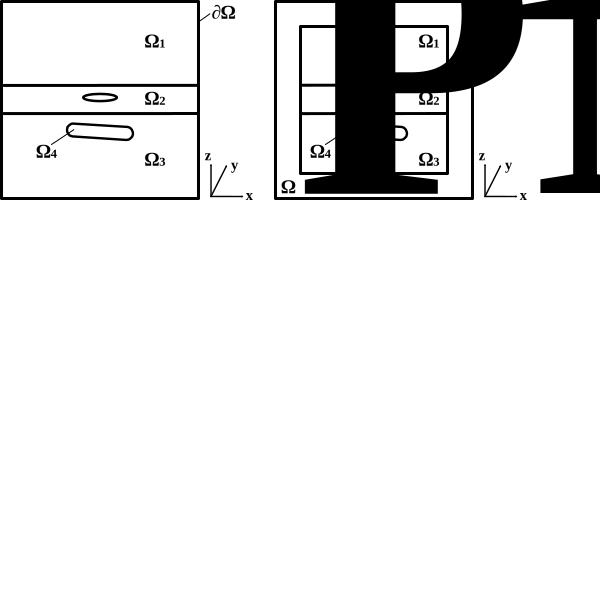
\includegraphics[trim=0mm 0mm 79.0mm 0mm,clip,scale=1]{theory/area_3layers_PML.eps}\label{fig:theory:area_3layers_PML_a}}
	\subfloat[][]{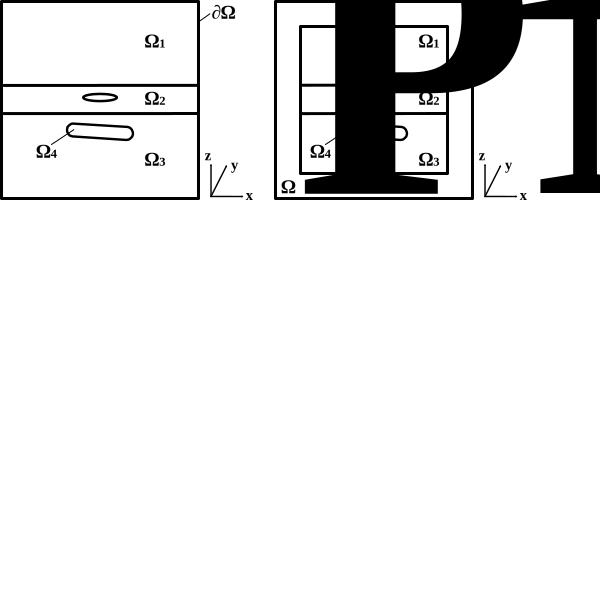
\includegraphics[trim=77.0mm 0mm 0mm 0mm,clip,scale=1]{theory/area_3layers_PML.eps}\label{fig:theory:area_3layers_PML_b}}
	\caption{расчётные области: (а) без PML-слоя и (б) с PML-слоем}
	\label{fig:theory:area_3layers_PML}
\end{figure}

PML-слой определяется модифицированными координатами $\tilde{x}$, $\tilde{y}$, $\tilde{z}$, полученными следующей заменой координат ~\citep{wiik_dehoop_ursin}:
\begin{equation*}
	\tilde{x} = \int\limits_0^x s_x (t) \,dt ,
	\text{~~~~~}
	\tilde{y} = \int\limits_0^y s_y (t) \,dt ,
	\text{~~~~~}
	\tilde{z} = \int\limits_0^z s_z (t) \,dt ,
\end{equation*}
где $s_j(\tau) = 1$ вне PML-слоя, а внутри него может быть задано в виде:
\begin{equation}
	s_j(\tau) = 1 + \chi \left( \frac{d(\tau)}{\delta} \right)^m , \text{~~} m \geq 1 ,
	\label{eq:pml_s}
\end{equation}
где $d(\tau)$ -- расстояние в $j$-м направлении от внутренней границы PML-слоя, $\delta$ -- толщина PML-слоя, $\chi$ -- некоторое комплексное число, причём $\Re(\chi) \ge 0$, $\Im(\chi) \ge 0$. Оператор $\nabla$ в новых координатах будет иметь вид:
\begin{equation*}
	\tilde{\nabla} = \left[ \frac{1}{s_x} \frac{\partial}{\partial x} \,, \frac{1}{s_y} \frac{\partial}{\partial y} \,, \frac{1}{s_z} \frac{\partial}{\partial z} \right] .
\end{equation*}
После такой замены, внутри PML-слоя уравнение Гельмгольца (\ref{eq:helmholtz}) будет иметь вид (\ref{eq:helmholtz_pml})
\begin{equation}
	\tilde{\nabla} \times ( \mu^{-1} \tilde{\nabla} \times \tilde{\mathbf{E}} ) + k^{2} \tilde{\mathbf{E}} = 0 , \label{eq:helmholtz_pml}
\end{equation}
что приведёт к преобразованию уравнения (\ref{eq:weak}) к виду (\ref{eq:weak_pml}):
\begin{equation}
	\int\limits_{{\Omega^{PML}}} \mu^{-1} \tilde{\nabla} \times \tilde{\mathbf{E}} \cdot \tilde{\nabla} \times \overline{\mathbf{v}} \,d{\Omega^{PML}} + \int\limits_{{\Omega^{PML}}} k^{2} \tilde{\mathbf{E}} \cdot \overline{\mathbf{v}} \,d{\Omega^{PML}} = 0 . \label{eq:weak_pml}
\end{equation}

В результате, если обозначить $\widehat{\Omega} = \Omega \setminus {\Omega^{PML}}$, то векторная вариационная постановка с учётом PML-слоя примет вид: \textbf{\textit{Найти $\mathbf{E} \in \mathbb{H}_{0}( \mathrm{rot}\,, \widehat{\Omega} )$ и  $\tilde{\mathbf{E}} \in \mathbb{H}_{0}( \mathrm{rot}\,, {\Omega^{PML}} )$, такие что $\forall \mathbf{v} \in \mathbb{H}_{0}( \mathrm{rot}\,, \widehat{\Omega} )$ и $\forall \tilde{\mathbf{v}} \in \mathbb{H}_{0}( \mathrm{rot}\,, {\Omega^{PML}} )$ будет выполнено}}:
\begin{equation*}
	\begin{cases}
		\displaystyle
		\int\limits_{\widehat{\Omega}} \mu^{-1} \nabla \times \mathbf{E} \cdot \nabla \times \overline{\mathbf{v}} \,d\widehat{\Omega} + \int\limits_{\widehat{\Omega}} k^{2} \mathbf{E} \cdot \overline{\mathbf{v}} \,d\widehat{\Omega} = - \int\limits_{\widehat{\Omega}} i \omega \mathbf{J} \cdot \overline{\mathbf{v}} \,d\widehat{\Omega} \\
		\displaystyle
		\int\limits_{{\Omega^{PML}}} \mu^{-1} \tilde{\nabla} \times \tilde{\mathbf{E}} \cdot \tilde{\nabla} \times \tilde{\overline{\mathbf{v}}} \,d{\Omega^{PML}} + \int\limits_{{\Omega^{PML}}} k^{2} \tilde{\mathbf{E}} \cdot \tilde{\overline{\mathbf{v}}} \,d{\Omega^{PML}} = 0 . \\
	\end{cases}
\end{equation*}

% =============================================================================

\subsection{Дискретная вариационная постановка}
Разобьём область $\Omega$ на $m$ непересекающихся элементов:
\begin{equation*}
	\Omega = \bigcup\limits_{k=1}^{m} \Omega_k , \text{~~} \forall i \neq j , \text{~~} \Omega_i \cap \Omega_j = \varnothing .
\end{equation*}

Введём конечномерные подпространства:
\begin{equation*}
	\mathbb{H}_{0}^h( \mathrm{rot}\,, \Omega ) \subset \mathbb{H}_{0}( \mathrm{rot}\,, \Omega ) , \text{~~}
	\mathbb{H}_{0}^h( \mathrm{grad}\,, \Omega ) \subset \mathbb{H}_{0}( \mathrm{grad}\,, \Omega ) .
\end{equation*}
Для дискретных подпространств $\mathbb{H}_{0}^h( \mathrm{rot}\,, \Omega )$ и $\mathbb{H}_{0}^h( \mathrm{grad}\,, \Omega )$ комплекс Де Рама~(\ref{eq:derham}) также будет верен, следовательно, закон сохранения заряда~(\ref{eq:charge}) будет также выполнен в слабом смысле~\citep{epov}.

Пространство $\mathbb{H}_{0}^h( \mathrm{rot}\,, \Omega )$ является прямой суммой подпространств~\citep{hiptmair,epov}
\begin{equation}
	\mathbb{H}_{0}^h( \mathrm{rot}\,, \Omega ) = \mathbb{N}_{0}^h( \mathrm{rot}\,, \Omega ) \oplus (\mathbb{N}_{0}^h( \mathrm{rot}\,, \Omega ))^{\bot} ,
	\label{eq:subspaces_sum}
\end{equation}
где $\mathbb{N}_{0}^h( \mathrm{rot}\,, \Omega )$ -- ядро rot-оператора, $(\mathbb{N}_{0}^h( \mathrm{rot}\,, \Omega ))^{\bot}$ -- его ортогональное дополнение. Для выполнения условий непрерывности (\ref{eq:maxwell:tangent_E})-(\ref{eq:maxwell:normal_D}) необходимо использовать полный базис (базис II типа) \citep{webb1993,webb1999,nedelec1980,nedelec1986,epov}, состоящий из двух типов базисных функций. Первый тип -- роторные базисные функции из пространства $(\mathbb{N}_{0}^h( \mathrm{rot}\,, \Omega ))^{\bot}$, которые обеспечивают непрерывность тангенциальных компонент электрического поля $\mathbf{E}$ (\ref{eq:maxwell:tangent_E}). Второй -- градиентные базисные функции из пространства $\mathbb{N}_{0}^h( \mathrm{rot}\,, \Omega )$, которые обеспечивают скачок нормальной компоненты электрического поля $\mathbf{E}$~(\ref{eq:maxwell:normal_D}) и выполнение закона сохранения заряда~(\ref{eq:charge}).

Представим векторнозначную функцию $\mathbf{E}^h$ в виде разложения по базису \linebreak $\boldsymbol{\psi}_j \in \mathbb{H}_{0}^h( \mathrm{rot}\,, \Omega )$:
\begin{equation*}
	\mathbf{E}^h = \sum\limits_{j = 1}^n q_j \boldsymbol{\psi}_j .
\end{equation*}
В качестве тестовой функции выберем базисную функцию $\boldsymbol{\psi}_i \in \mathbb{H}_{0}^h( \mathrm{rot}\,, \Omega )$, тогда конечноэлементная аппроксимация вариационного уравнения (\ref{eq:weak}) примет вид:
\begin{equation}
	\begin{array}{c} { \displaystyle
		\sum\limits_{j = 1}^n \left( \int\limits_\Omega \mu^{-1} \nabla \times \boldsymbol{\psi}_j \cdot \nabla \times \boldsymbol{\psi}_i \,d\Omega + \int\limits_\Omega k^{2} \boldsymbol{\psi}_j \cdot \boldsymbol{\psi}_i \,d\Omega \right) q_j =
	} \\ { \displaystyle
		=  - \int\limits_\Omega i \omega \mathbf{J} \cdot \boldsymbol{\psi}_i \,d\Omega .
	} \end{array}
	\label{eq:weak_discr}
\end{equation}

В матрично-векторной форме (\ref{eq:weak_discr}) можно представить в виде следующей системы линейных алгебраических уравнений (СЛАУ):
\begin{equation}
	( \mathbf{G} + \mathbf{M} )\mathbf{q} = \mathbf{f} , \label{eq:form_29}
\end{equation}
%где:
\begin{equation*}
	\mathbf{G}_{ i,j } = \int\limits_{\Omega_k} \mu^{-1} \nabla \times \mathbf{w}_i \cdot \nabla \times \mathbf{w}_j \,d\Omega_k , \text{~~~}
	\mathbf{M}_{ i,j } = \int\limits_{\Omega_k} k^2 \mathbf{w}_i \cdot \mathbf{w}_j \,d\Omega_k . \label{eq:local_matrixes}
\end{equation*}

Матрица СЛАУ будет иметь симметричную разреженную структуру, поэтому её удобно хранить в формате CSLR~(Compressed Sparse (Lower triangle) Row) или CSR~(Compressed Sparse Row)~\citep{balandin_slae}.
% Система линейных алгебраических уравнений (СЛАУ) (\ref{eq:slae}) решается специальным двухуровневым методом~\citep{nechaev}.

% =============================================================================

\subsection{Тетраэдральные конечные элементы}

В качестве конечных элементов для представления расчётной области, будем пользоваться тетраэдрами. На тетраэдральном конечном элементе определим $\mathcal{L}$-ко\-ор\-ди\-на\-ты, называемые также барицентрическими координатами~\citep{soloveychick}. Введём нумерацию вершин и рёбер, показанную на рисунке \ref{fig:theory:tetrahedron}:
\begin{figure}[H]
	\centering
	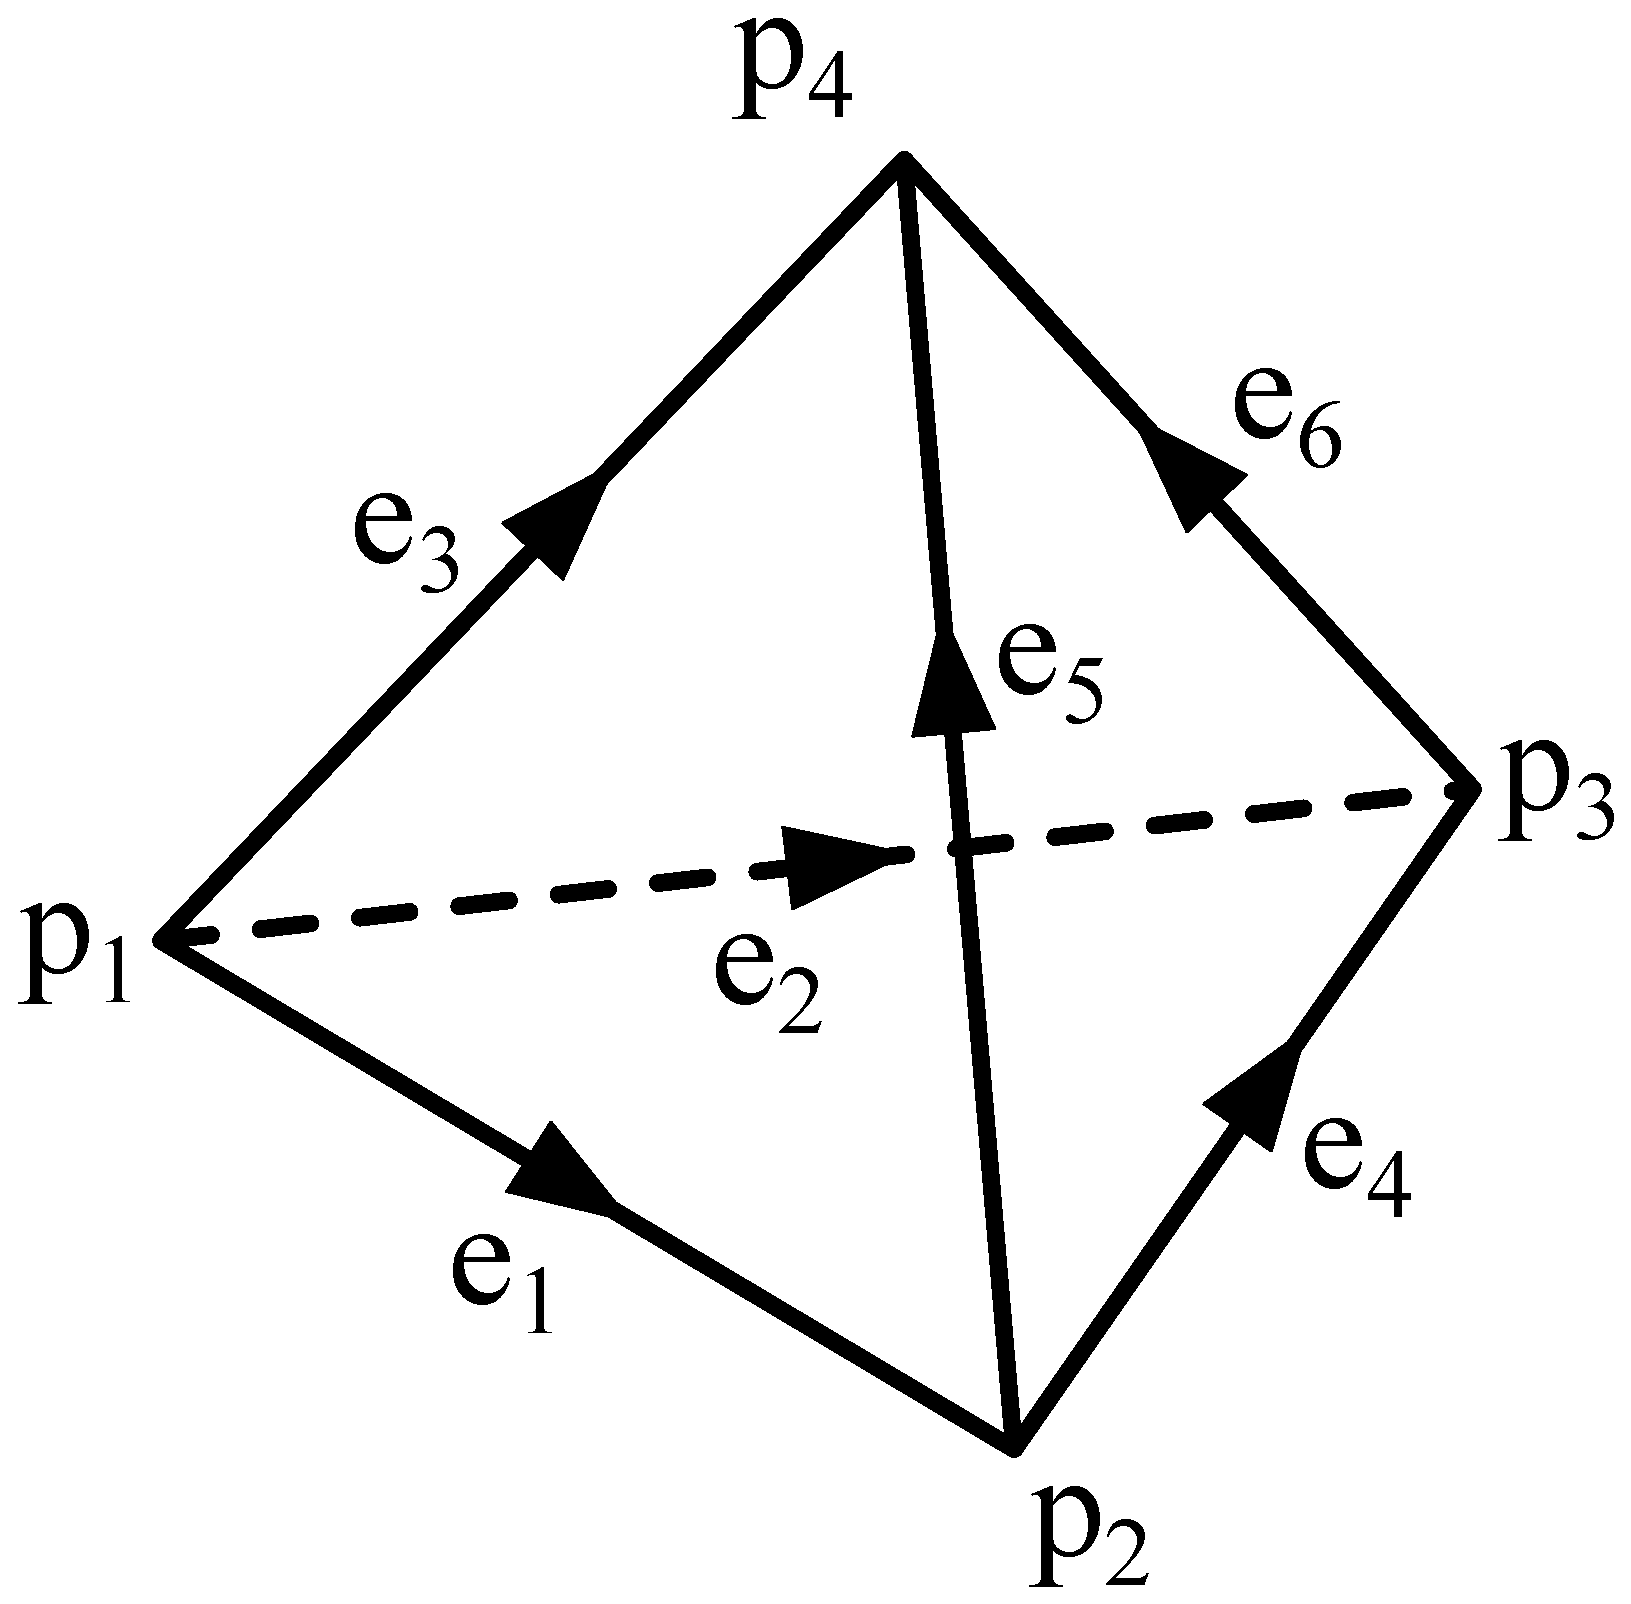
\includegraphics[scale=0.25]{theory/tetrahedron.eps}
	\caption{тетраэдральный конечный элемент}
	\label{fig:theory:tetrahedron}
\end{figure}

\noindent Под $\mathcal{L}$-координатами понимают функции следующего вида:
\begin{equation*}
	\mathcal{L}_i (x, y, z) = \alpha_{i, 1} x + \alpha_{i, 2} y + \alpha_{i, 3} z + \alpha_{i, 4} , \text{~~~} i = \overline{1..4} . \label{eq:tet:L}
\end{equation*}
Коэффициенты $\alpha_{i, j}$ могут быть определены по формуле (\ref{eq:tet:D1}):
\begin{equation}
	\left[
	\begin{matrix}
		\alpha_{1, 1} & \alpha_{1, 2} & \alpha_{1, 3} & \alpha_{1, 4} \\
		\alpha_{2, 1} & \alpha_{2, 2} & \alpha_{2, 3} & \alpha_{2, 4} \\
		\alpha_{3, 1} & \alpha_{3, 2} & \alpha_{3, 3} & \alpha_{3, 4} \\
		\alpha_{4, 1} & \alpha_{4, 2} & \alpha_{4, 3} & \alpha_{4, 4} \\
	\end{matrix}
	\right] = \left[
	\begin{matrix}
		{p_1}_x & {p_2}_x & {p_3}_x & {p_4}_x \\
		{p_1}_y & {p_2}_y & {p_3}_y & {p_4}_y \\
		{p_1}_z & {p_2}_z & {p_3}_z & {p_4}_z \\
		1 & 1 & 1 & 1 \\
	\end{matrix}
	\right]^{-1} . \label{eq:tet:D1}
\end{equation}

Задав $\mathcal{L}$-координаты, можно определить на тетраэдре базисные функции. В отличие от узлового метода конечных элементов, в векторном методе конечных элементов базисные функции ассоциированы не с узлами, а с рёбрами (edge), гранями (face) и объёмами (volume)~\citep{nechaev, webb1999}. Так как будут использованы полные (II типа) базисы первого и второго порядков, то ограничимся рассмотрением только базисных функций, ассоциированных с рёбрами и гранями.

Иерархический векторный базис Вебба второго порядка второго типа на тетраэдрах имеет вид~\citep{mikhajlova}:
\begin{equation}
	\begin{matrix}
		\displaystyle
		\mathbf{w}_{i}^{1,\mathrm{I}} = \mathcal{L}_k \nabla \mathcal{L}_l - \mathcal{L}_l \nabla \mathcal{L}_k ;
		\scriptstyle
		\text{~~} i = 1, ..., 6 ; \text{~~} k, l = 1, ..., 4 ; \text{~~} k < l ,\\
		\displaystyle
		\mathbf{w}_{i}^{1,\mathrm{II}} = \mathcal{L}_k \nabla \mathcal{L}_l + \mathcal{L}_l \nabla \mathcal{L}_k ;
		\scriptstyle
		\text{~~} i = 7, ..., 12 ; \text{~~} k, l = 1, ..., 4 ; \text{~~} k < l ,\\
		\displaystyle
		\mathbf{w}_{i}^{2,\mathrm{I}} = \mathcal{L}_k \mathcal{L}_l \nabla \mathcal{L}_j + \mathcal{L}_j \mathcal{L}_l \nabla \mathcal{L}_k - 2 \mathcal{L}_j \mathcal{L}_k \nabla \mathcal{L}_l ;
		\scriptstyle
		\text{~~} i = 13, ..., 16 ; \text{~~} j, k, l = 1, ..., 4 ; \text{~~} j < k < l ,\\
		\displaystyle
		\mathbf{w}_{i}^{2,\mathrm{I}} = \mathcal{L}_k \mathcal{L}_l \nabla \mathcal{L}_j - 2 \mathcal{L}_j \mathcal{L}_l \nabla \mathcal{L}_k + \mathcal{L}_j \mathcal{L}_k \nabla \mathcal{L}_l ;
		\scriptstyle
		\text{~~} i = 17, ..., 20 ; \text{~~} j, k, l = 1, ..., 4 ; \text{~~} j < k < l ,\\
		\displaystyle
		\mathbf{w}_{i}^{2,\mathrm{II}} = \nabla ( \mathcal{L}_j \mathcal{L}_k \mathcal{L}_l ) ;
		\scriptstyle
		\text{~~} i = 21, ..., 24 ; \text{~~} j, k, l = 1, ..., 4 ; \text{~~} j < k < l ,\\
		\displaystyle
		\mathbf{w}_{i}^{2,\mathrm{II}} = \nabla ( \mathcal{L}_j \mathcal{L}_k ( \mathcal{L}_j - \mathcal{L}_k ) ) ;
		\scriptstyle
		\text{~~} i = 25, ..., 30 ; \text{~~} j, k = 1, ..., 4 ; \text{~~} j < k ,
	\end{matrix}
	\label{eq:basis}
\end{equation}
где $\mathbf{w}_{1}^{1,\mathrm{I}}, ..., \mathbf{w}_{6}^{1,\mathrm{I}}$ -- базисные функции первого порядка первого типа, ассоциированные с рёбрами, $\mathbf{w}_{7}^{1,\mathrm{II}}, ..., \mathbf{w}_{12}^{1,\mathrm{II}}$ -- базисные функции первого порядка второго типа, ассоциированные с рёбрами, $\mathbf{w}_{13}^{2,\mathrm{I}}, ..., \mathbf{w}_{20}^{2,\mathrm{I}}$ -- базисные функции второго порядка первого типа, ассоциированные с гранями, $\mathbf{w}_{21}^{2,\mathrm{II}}, ..., \mathbf{w}_{24}^{2,\mathrm{II}}$ -- базисные функции второго порядка второго типа, ассоциированные с гранями, $\mathbf{w}_{25}^{2,\mathrm{II}}, ..., \mathbf{w}_{30}^{2,\mathrm{II}}$ -- базисные функции второго порядка второго типа, ассоциированные с рёбрами. Так как этот базис иерархический, то для получения базиса меньшего порядка следует ограничиться меньшим количеством функций. Так, для базиса первого порядка второго  типа следует использовать функции $\mathbf{w}_{1}^{1,\mathrm{I}}, ..., \mathbf{w}_{12}^{1,\mathrm{II}}$.

Для вычисления интегралов в (\ref{eq:weak_discr}) воспользуемся кубатурной формулой численного интегрирования (формулой Гаусса)~\citep{misovskih}:
\begin{equation*}
	\int\limits_{\Omega_k} f(x, y, z) \,d\Omega_k = \sum\limits_{i = 1}^m f( x_i , y_i , z_i ) w_i ,
\end{equation*}
где $(x_i , y_i , z_i )$ -- точки Гаусса, $m$ -- число точек Гаусса, $w_i$ -- соответствующие веса. При работе с базисными функциями второго порядка нужно использовать формулы, которые бы обеспечивали восьмой порядок интегрирования~\citep{zhang_integration}. Для базисных функций первого порядка будет достаточно и меньших порядков интегрирования~\citep{tet_integration, misovskih}.

% =============================================================================

\subsection{Треугольные конечные элементы}

Границы области $\Omega$ являются двумерными и представляют собой треугольники. Для учёта краевых условий (\ref{eq:bound1}) требуется построить разложение $\mathbf{E}^g$ по базису соответствующей границы в смысле МНК, для этого нужно решать СЛАУ вида
\begin{equation}
	\mathbf{M}^{S_1} \tilde{\mathbf{q}} = \mathbf{b}^{S_1} ,
	\label{eq:bound_mnk}
\end{equation}
где $\displaystyle \mathbf{M}^{S_1}_{i,j} = \int\limits_{S_1} \tilde{\mathbf{w}}_i \cdot \tilde{\mathbf{w}}_j \,d S_1$, $\displaystyle \mathbf{b}^{S_1}_{i} = \int\limits_{S_1} \mathbf{E}^g \cdot \tilde{\mathbf{w}}_i \,d S_1$, $\tilde{\mathbf{w}}_i$ и $\tilde{\mathbf{w}}_j$ -- базисные функции на треугольниках.

Определим $\mathcal{L}$-координаты на треугольниках таким же образом, как и на тетраэдрах. Введём нумерацию вершин и рёбер согласно рисунку \ref{fig:theory:triangle}:
\begin{figure}[H]
	\centering
	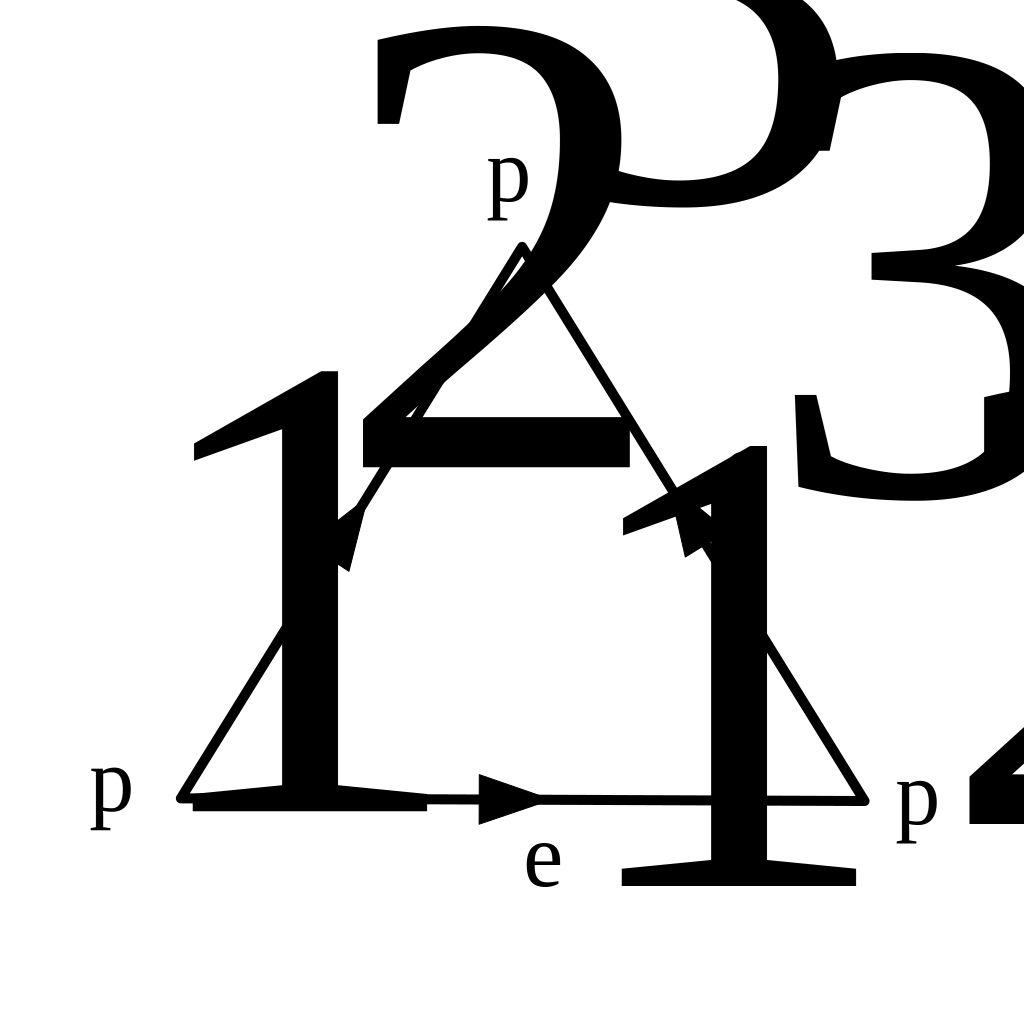
\includegraphics[scale=0.25]{theory/triangle.eps}
	\caption{треугольный конечный элемент}
	\label{fig:theory:triangle}
\end{figure}

\noindent Тогда $\mathcal{L}$-координаты примут вид:
\begin{equation*}
	\mathcal{L}_i (x, y) = \alpha_{i, 1} x + \alpha_{i, 2} y + \alpha_{i, 3} , \text{~~~} i = \overline{1..3} . \label{eq:tr:L}
\end{equation*}
Коэффициенты $\alpha_{i, j}$ могут быть определены по формуле (\ref{eq:tr:D1}):
\begin{equation}
	\left[
	\begin{matrix}
		\alpha_{1, 1} & \alpha_{1, 2} & \alpha_{1, 3} \\
		\alpha_{2, 1} & \alpha_{2, 2} & \alpha_{2, 3} \\
		\alpha_{3, 1} & \alpha_{3, 2} & \alpha_{3, 3} \\
	\end{matrix}
	\right] = \left[
	\begin{matrix}
		{p_1}_x & {p_2}_x & {p_3}_x \\
		{p_1}_y & {p_2}_y & {p_3}_y \\
		1 & 1 & 1 \\
	\end{matrix}
	\right]^{-1} . \label{eq:tr:D1}
\end{equation}

Иерархический векторный базис Вебба второго порядка второго типа на треугольниках имеет вид:
\begin{equation*}
	\begin{matrix}
		\displaystyle
		\tilde{\mathbf{w}}_{i}^{1,\mathrm{I}} = \mathcal{L}_k \nabla \mathcal{L}_l - \mathcal{L}_l \nabla \mathcal{L}_k ;
		\scriptstyle
		\text{~~} i = 1, ..., 3 ; \text{~~} k, l = 1, ..., 3 ; \text{~~} k < l ,\\
		\displaystyle
		\tilde{\mathbf{w}}_{i}^{1,\mathrm{II}} = \mathcal{L}_k \nabla \mathcal{L}_l + \mathcal{L}_l \nabla \mathcal{L}_k ;
		\scriptstyle
		\text{~~} i = 4, ..., 6 ; \text{~~} k, l = 1, ..., 3 ; \text{~~} k < l ,\\
		\displaystyle
		\tilde{\mathbf{w}}_{7}^{2,\mathrm{I}} = \mathcal{L}_2 \mathcal{L}_3 \nabla \mathcal{L}_1 + \mathcal{L}_1 \mathcal{L}_3 \nabla \mathcal{L}_2 - 2 \mathcal{L}_1 \mathcal{L}_2 \nabla \mathcal{L}_3 ,\\
		\displaystyle
		\tilde{\mathbf{w}}_{8}^{2,\mathrm{I}} = \mathcal{L}_2 \mathcal{L}_3 \nabla \mathcal{L}_1 - 2 \mathcal{L}_1 \mathcal{L}_3 \nabla \mathcal{L}_2 + \mathcal{L}_1 \mathcal{L}_2 \nabla \mathcal{L}_3 ,\\
		\displaystyle
		\tilde{\mathbf{w}}_{9}^{2,\mathrm{II}} = \nabla ( \mathcal{L}_1 \mathcal{L}_2 \mathcal{L}_3 ) ,\\
		\displaystyle
		\tilde{\mathbf{w}}_{i}^{2,\mathrm{II}} = \nabla ( \mathcal{L}_j \mathcal{L}_k ( \mathcal{L}_j - \mathcal{L}_k ) ) ;
		\scriptstyle
		\text{~~} i = 10, ..., 12 ; \text{~~} j, k = 1, ..., 3 ; \text{~~} j < k ,
	\end{matrix}
	\label{eq:tr_basis}
\end{equation*}
где $\tilde{\mathbf{w}}_{1}^{1,\mathrm{I}}, ..., \tilde{\mathbf{w}}_{3}^{1,\mathrm{I}}$ -- базисные функции первого порядка первого типа, $\tilde{\mathbf{w}}_{4}^{1,\mathrm{II}}, ..., \tilde{\mathbf{w}}_{6}^{1,\mathrm{II}}$ -- базисные функции первого порядка второго типа, $\tilde{\mathbf{w}}_{7}^{2,\mathrm{I}}, \tilde{\mathbf{w}}_{8}^{2,\mathrm{I}}$ -- базисные функции второго порядка первого типа, $\tilde{\mathbf{w}}_{9}^{2,\mathrm{II}}, ..., \tilde{\mathbf{w}}_{12}^{2,\mathrm{II}}$ -- базисные функции второго порядка второго типа. Для базиса первого порядка второго типа следует использовать функции $\tilde{\mathbf{w}}_{1}^{1,\mathrm{I}}, ..., \tilde{\mathbf{w}}_{6}^{1,\mathrm{II}}$.

Для вычисления интегралов в (\ref{eq:bound_mnk}) воспользуемся формулой Гаусса~\citep{misovskih}:
\begin{equation*}
	\int\limits_{\Omega_k} f(x, y) \,d\Omega_k = \sum\limits_{i = 1}^m f( x_i , y_i) w_i ,
\end{equation*}
где $(x_i , y_i)$ -- точки Гаусса, $m$ -- число точек Гаусса, $w_i$ -- соответствующие веса. Так же, как и для тетраэдров, для работы с базисом второго порядка нужно использовать формулы, обеспечивающие восьмой порядок интегрирования~\citep{zhang_integration}. Для базиса первого порядка достаточно и меньших порядков интегрирования~\citep{tr_integration, misovskih}.

% =============================================================================

\subsection{Двухуровневый решатель}
Так как пространство $\mathbb{H}_{0}^h( \mathrm{rot}\,, \Omega )$ представимо в виде прямой суммы подпространств~(\ref{eq:subspaces_sum}), можно построить специальный двухуровневый решатель, который учитывает ядро $\mathrm{rot}$-оператора. Принцип построения подробно изложен в~\citep{nechaev, shokin_multigrid}.

Рассмотрим иерархический узловой базис пространства $\mathbb{H}_{0}^h( \mathrm{grad}\,, \Omega )$ на тетраэдре:
\begin{equation*}
	\begin{matrix}
		\displaystyle
		\phi_{i} = \mathcal{L}_i ;
		\scriptstyle
		\text{~~} i = 1, ..., 4 ,\\
		\displaystyle
		\phi_{i} = \mathcal{L}_k \mathcal{L}_l ;
		\scriptstyle
		\text{~~} i = 5, ..., 10 ; \text{~~} k, l = 1, ..., 4 ; \text{~~} k < l ,\\
		\displaystyle
		\phi_{i} = \mathcal{L}_j \mathcal{L}_k \mathcal{L}_l ;
		\scriptstyle
		\text{~~} i = 11, ..., 14 ; \text{~~} j, k, l = 1, ..., 4 ; \text{~~} j < k < l ,\\
		\displaystyle
		\phi_{i} = \mathcal{L}_j \mathcal{L}_k ( \mathcal{L}_j - \mathcal{L}_k ) ;
		\scriptstyle
		\text{~~} i = 15, ..., 20 ; \text{~~} j, k = 1, ..., 4 ; \text{~~} j < k .
	\end{matrix}
	\label{eq:basis_nodal}
\end{equation*}
Градиенты этих базисных функций принадлежат пространству $\mathbb{H}_{0}^h( \mathrm{rot}\,, \Omega )$:
\begin{equation}
	\begin{matrix}
		\displaystyle
		\nabla \phi_{1} = \nabla \mathcal{L}_1 = - \mathbf{w}_{1}^{1,\mathrm{I}} - \mathbf{w}_{2}^{1,\mathrm{I}} - \mathbf{w}_{3}^{1,\mathrm{I}} ,\\
		\displaystyle
		\nabla \phi_{2} = \nabla \mathcal{L}_2 = \mathbf{w}_{1}^{1,\mathrm{I}} - \mathbf{w}_{4}^{1,\mathrm{I}} + \mathbf{w}_{5}^{1,\mathrm{I}} ,\\
		\displaystyle
		\nabla \phi_{3} = \nabla \mathcal{L}_3 = \mathbf{w}_{2}^{1,\mathrm{I}} + \mathbf{w}_{4}^{1,\mathrm{I}} - \mathbf{w}_{6}^{1,\mathrm{I}} ,\\
		\displaystyle
		\nabla \phi_{4} = \nabla \mathcal{L}_4 = \mathbf{w}_{3}^{1,\mathrm{I}} - \mathbf{w}_{5}^{1,\mathrm{I}} + \mathbf{w}_{6}^{1,\mathrm{I}} ,\\
		\displaystyle
		\nabla \phi_{i} = \nabla ( \mathcal{L}_k \mathcal{L}_l ) = \mathbf{w}_{i+2}^{1,\mathrm{II}} ;
		\scriptstyle
		\text{~~} i = 5, ..., 10 ; \text{~~} k, l = 1, ..., 4 ; \text{~~} k < l ,\\
		\displaystyle
		\nabla \phi_{i} = \nabla ( \mathcal{L}_j \mathcal{L}_k \mathcal{L}_l ) = \mathbf{w}_{i+10}^{2,\mathrm{II}} ;
		\scriptstyle
		\text{~~} i = 11, ..., 14 ; \text{~~} j, k, l = 1, ..., 4 ; \text{~~} j < k < l ,\\
		\displaystyle
		\nabla \phi_{i} = \nabla ( \mathcal{L}_j \mathcal{L}_k ( \mathcal{L}_j - \mathcal{L}_k ) ) = \mathbf{w}_{i+10}^{2,\mathrm{II}} ;
		\scriptstyle
		\text{~~} i = 15, ..., 20 ; \text{~~} j, k = 1, ..., 4 ; \text{~~} j < k .
	\end{matrix}
	\label{eq:basis_nodal_grads}
\end{equation}
Таким образом мы можем построить матрицу перехода $\mathbf{P}$ от базиса $\mathbf{w}$~(\ref{eq:basis}) к базису $\nabla \phi$~(\ref{eq:basis_nodal_grads}). В силу иерархичности базисов, матрица $\mathbf{P}$ будет иметь блочную структуру. Матрицы перехода для базисов различных порядков имеют вид:
\begin{equation*}
	\mathbf{P}^{1,I} = \left[
	\begin{matrix}
		-1 & -1 & -1 &  0 &  0 &  0 \\
		 1 &  0 &  0 & -1 & -1 &  0 \\
		 0 &  1 &  0 &  1 &  0 & -1 \\
		 0 &  0 &  1 &  0 &  1 &  1 \\
	\end{matrix}
	\right],
\text{~~~~}
	\mathbf{P}^{1,II} = \left[
	\begin{matrix}
		\mathbf{P}^{1,I} & \mathbb{O}_{4 \times 6} \\
		\mathbb{O}_{6 \times 6} & \mathbf{I}_{6 \times 6} \\
	\end{matrix}
	\right],
\end{equation*}
\begin{equation*}
	\mathbf{P}^{2,I} = \left[
	\begin{matrix}
		\mathbf{P}^{1,II} & \mathbb{O}_{10 \times 8} \\
	\end{matrix}
	\right],
\text{~~~~~~~~~~~~~~~~}
	\mathbf{P}^{2,II} = \left[
	\begin{matrix}
		\mathbf{P}^{2,I} & \mathbb{O}_{10 \times 10} \\
		\mathbb{O}_{10 \times 20} & \mathbf{I}_{10 \times 10} \\
	\end{matrix}
	\right],
\end{equation*}
где $\mathbf{I}_{n \times n}$ -- единичная матрица размерностью $n \times n$, $\mathbb{O}_{n \times m}$ -- нулевая матрица размерностью $n \times m$.

\pagebreak
Общий алгоритм многоуровневых методов имеет следующий вид:
\begin{enumerate}
	\item \label{itm:multilevel:algo1} Выбрать некоторое начальное приближение;
	\item \label{itm:multilevel:algo2} Уточнить решение на полном пространстве (подавить высокочастотную составляющую ошибки);
	\item \label{itm:multilevel:algo3} Спроектировать приближение с шага \ref{itm:multilevel:algo2} на грубое подпространство;
	\item \label{itm:multilevel:algo4} Уточнить решение на грубом подпространстве (подавить низкочастотную составляющую ошибки);
	\item \label{itm:multilevel:algo5} Интерполировать решение на полное подпространство;
	\item \label{itm:multilevel:algo6} Повторить шаги \ref{itm:multilevel:algo2} - \ref{itm:multilevel:algo5} пока не будет достигнута нужная точность.
\end{enumerate}

Псевдокод алгоритма двухуровневого метода:

\vspace{1em}
\begin{algorithm}[H]
	\SetAlgoLined
	\KwIn{ $\mathbf{A}$, $\mathbf{f}$, $\mathbf{q}_0$, $\mathbf{P}$, $\gamma$, $\varepsilon_1$, $\varepsilon_2$ }
	\KwResult{ $\mathbf{q}$ }
	$\mathbf{r}_0 = \mathbf{f} - \mathbf{A} \mathbf{q}_0$ \\
	\For{$i = 1, 2, ...$ \textbf{пока} $\| \mathbf{r}_i \| > \gamma \| \mathbf{r}_0 \|$}
	{
		$\tilde{\mathbf{z}} = solve(\mathbf{P} \mathbf{A} \mathbf{P}^T , \mathbf{P} \mathbf{r}_{i-1} , \varepsilon_1 )$ \\
		$\tilde{\mathbf{q}}_{i} = \mathbf{q}_{i-1} + \mathbf{P}^T \tilde{\mathbf{z}}$ \\
		$\tilde{\mathbf{r}}_{i} = \mathbf{f} - \mathbf{A} \tilde{\mathbf{q}}_{i}$ \\
		$\mathbf{z} = solve(\mathbf{A}, \tilde{\mathbf{r}}_{i}, \varepsilon_2)$ \\
		$\mathbf{q}_{i} = \tilde{\mathbf{q}}_{i} + \mathbf{z}$ \\
		$\mathbf{r}_{i} = \mathbf{f} - \mathbf{A} \mathbf{q}_{i}$
	}
	$\mathbf{q} = \mathbf{q}_{i}$
\end{algorithm}
\vspace{1em}

\noindent где $\mathbf{A}$ и $\mathbf{f}$ -- матрица и правая часть СЛАУ~(\ref{eq:form_29}); $\mathbf{q}_0$ -- начальное приближение;  $\mathbf{P}$ -- матрица перехода от базиса $\mathbf{w}$~(\ref{eq:basis}) к базису $\nabla \phi$~(\ref{eq:basis_nodal_grads}); $\gamma$ -- точность решения СЛАУ; $\varepsilon_1$ и $\varepsilon_2$ -- точности решения промежуточных СЛАУ на подпространстве ядра и полном пространстве соответственно; $solve(\mathbf{A}, \mathbf{b}, \varepsilon)$ -- процедура решения СЛАУ с матрицей $\mathbf{A}$ и правой частью $\mathbf{b}$ с точностью $\varepsilon$.

В качестве $solve(\mathbf{A}, \mathbf{b}, \varepsilon)$ можно воспользоваться методами на подпространствах Крылова~\citep{balandin_slae, solver_saad, solver_iterative, solver_templates}, например, GMRES или COCG. Величины $\varepsilon_1$ и $\varepsilon_2$ следует выбирать небольшими, от $0.9$ до $0.01$~\citep{nechaev}.
%

% =============================================================================

\clearpage
\section{Построение и решение СЛАУ}
\labelname{2}\label{sec:build_slae}
\subsection{Структура глобальной матрицы СЛАУ}
Рассмотрим структуру глобальной матрицы СЛАУ на примере двух тетраэдральных конечных элементов с базисом первого полного порядка, имеющих общую грань. Глобальная нумерация вершин и рёбер этих тетраэдров приведена на рисунке \ref{fig:theory:2-tetrahedrons}.
\begin{figure}[H]
	\centering
	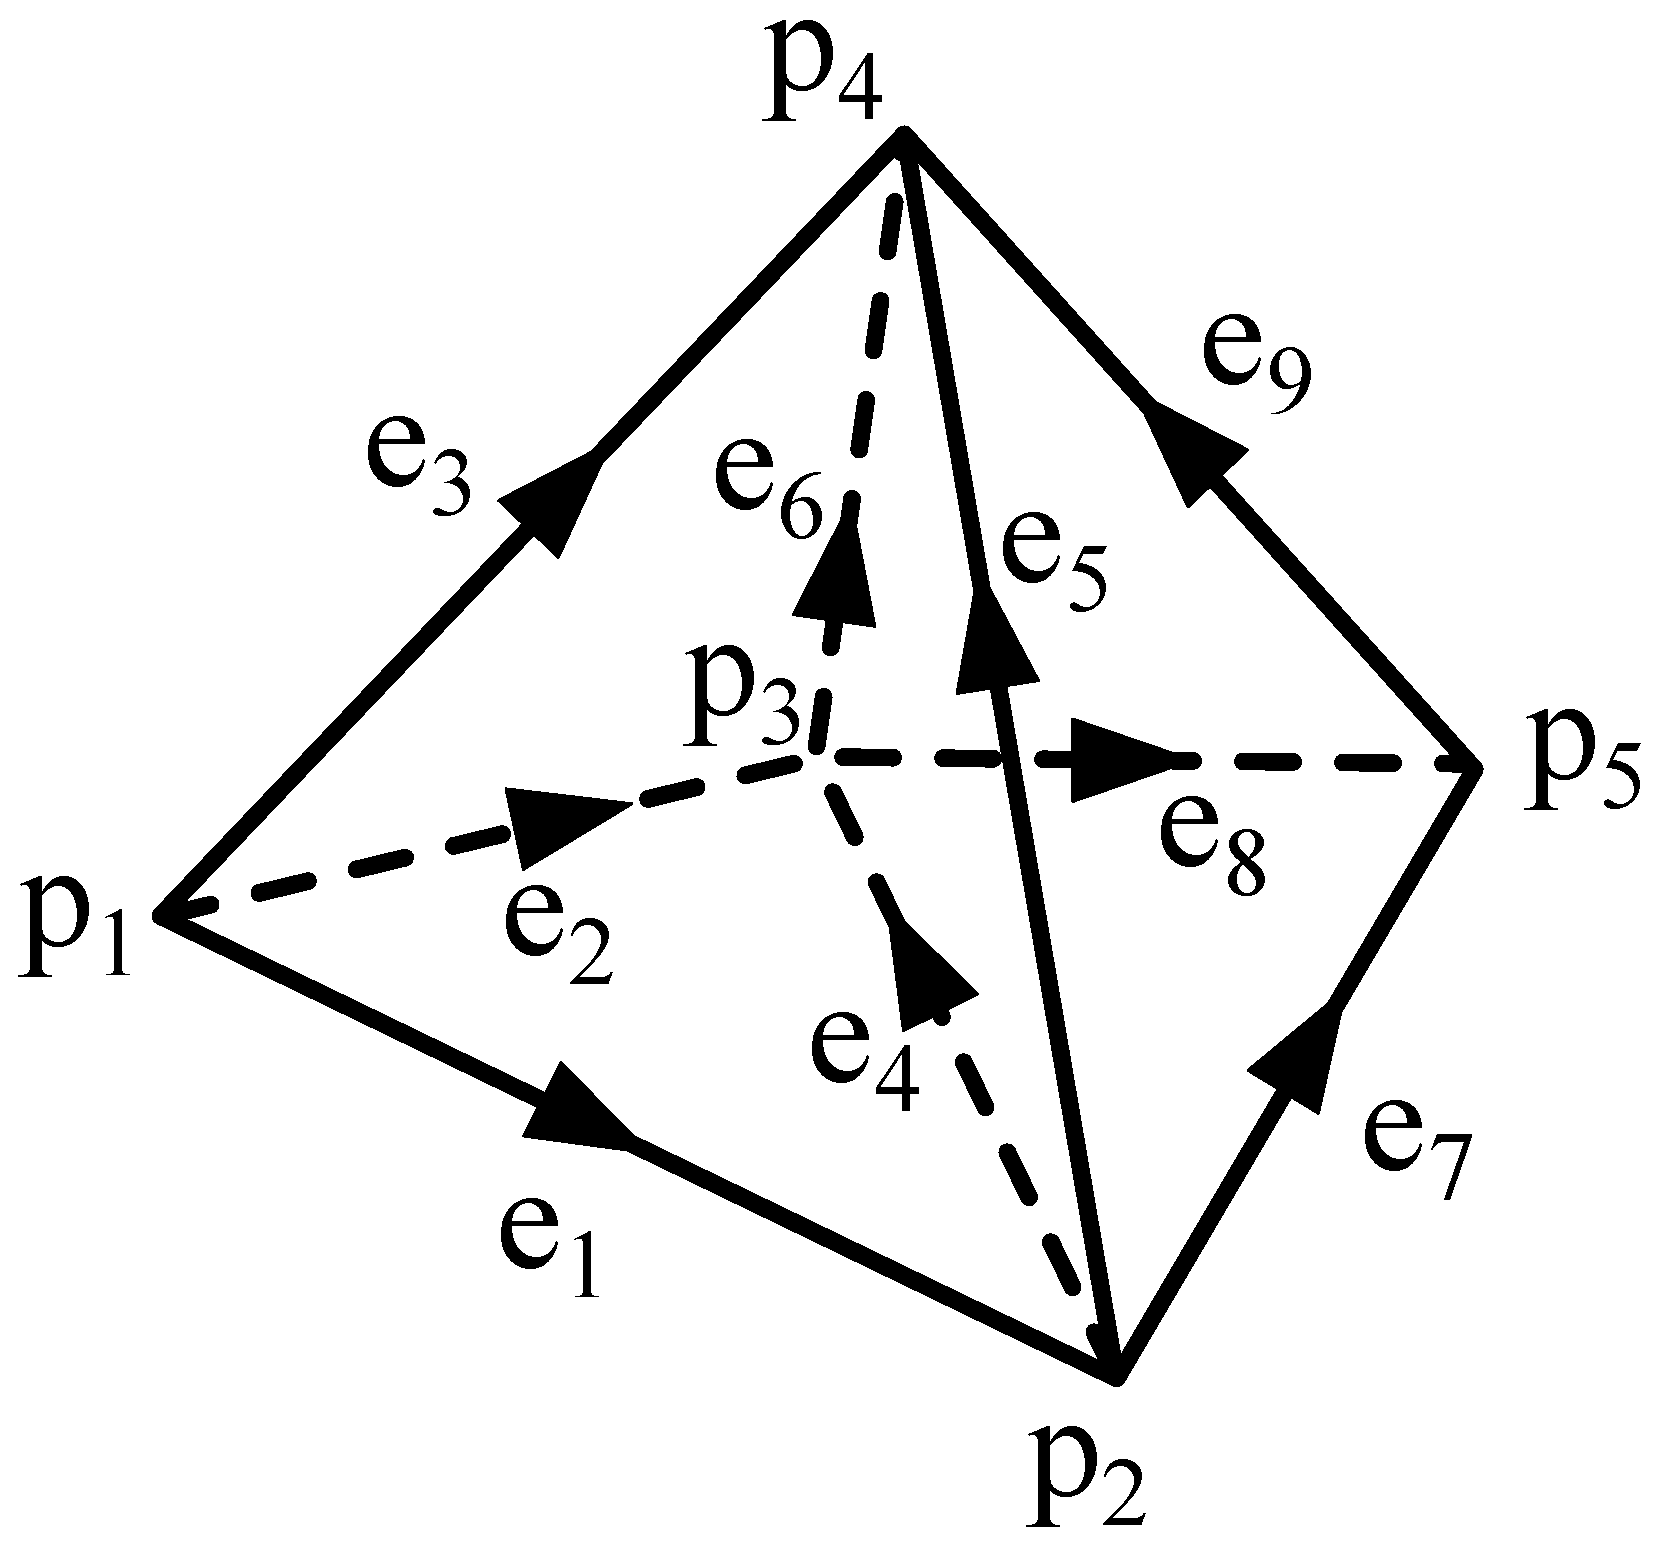
\includegraphics[scale=0.25]{theory/2-tetrahedrons.eps}
	\caption{два тетраэдральных конечных элемента}
	\label{fig:theory:2-tetrahedrons}
\end{figure}

Локальные матрицы тетраэдра имеют блочный вид, матрица массы является плотной (\ref{eq:theory:matrix_M}), а в матрице жёсткости ненулевой только один блок (\ref{eq:theory:matrix_G}):
\begin{equation}
	\mathbf{M} = \left[
	\begin{matrix}
		\mathbf{M}^{I, I} & \mathbf{M}^{I, II} \\
		\mathbf{M}^{II, I} & \mathbf{M}^{II, II} \\
	\end{matrix}
	\right] , \label{eq:theory:matrix_M}
\end{equation}
\begin{equation}
	\mathbf{G} = \left[
	\begin{matrix}
		\mathbf{G}^{I, I} & \mathbb{O} \\
		\mathbb{O} &  \mathbb{O} \\
	\end{matrix}
	\right] , \label{eq:theory:matrix_G}
\end{equation}
где $\mathbf{M}^{I, I}$, $\mathbf{G}^{I, I}$ -- блоки от интегралов, содержащих только роторные ($\mathbf{w}_{1}^{1,\mathrm{I}}, ..., \mathbf{w}_{6}^{1,\mathrm{I}}$); $\mathbf{M}^{II, II}$ -- только градиентные ($\mathbf{w}_{7}^{1,\mathrm{II}}, ..., \mathbf{w}_{12}^{1,\mathrm{II}}$); $\mathbf{M}^{I, II}$, $\mathbf{M}^{II, I}$ -- и роторные, и градиентные базисные функции.

Глобальная матрица также имеет блочную структуру, для двух тетраэдров она схематично приведена на рисунке \ref{fig:theory:matrx_structure}. Под $G_1$ и $G_2$ понимаются элементы матриц жёсткости (\ref{eq:theory:matrix_G}) первого и второго тетраэдров соответственно, под $M_1$ и $M_2$ -- элементы матриц массы (\ref{eq:theory:matrix_M}) первого и второго тетраэдров соответственно.

\begin{figure}[H]
	\begin{spacing}{0.75}
	\setlength{\parskip}{0pt}
	\begin{tabu}{|[2pt]@{}C{1}|@{}C{1}|@{}C{1}|@{}C{1}|@{}C{1}|@{}C{1}|@{}C{1}|@{}C{1}|@{}C{1}|[1.25pt]@{}C{1}|@{}C{1}|@{}C{1}|@{}C{1}|@{}C{1}|@{}C{1}|@{}C{1}|@{}C{1}|@{}C{1}|[2pt]}
		\tabucline[2pt]{-}
			~\vspace{-1ex}\par\small $\scriptscriptstyle G_{1} + M_{1}$ &
			~\vspace{-1ex}\par\small $\scriptscriptstyle G_{1} + M_{1}$ &
			~\vspace{-1ex}\par\small $\scriptscriptstyle G_{1} + M_{1}$ &
			~\vspace{-1ex}\par\small $\scriptscriptstyle G_{1} + M_{1}$ &
			~\vspace{-1ex}\par\small $\scriptscriptstyle G_{1} + M_{1}$ &
			~\vspace{-1ex}\par\small $\scriptscriptstyle G_{1} + M_{1}$ &
			&
			&
			&
			~\vspace{-1ex}\par~~\small $\scriptscriptstyle M_{1}$ &
			~\vspace{-1ex}\par~~\small $\scriptscriptstyle M_{1}$ &
			~\vspace{-1ex}\par~~\small $\scriptscriptstyle M_{1}$ &
			~\vspace{-1ex}\par~~\small $\scriptscriptstyle M_{1}$ &
			~\vspace{-1ex}\par~~\small $\scriptscriptstyle M_{1}$ &
			~\vspace{-1ex}\par~~\small $\scriptscriptstyle M_{1}$ &
			&
			&
		\\[0.75ex]\hline
			~\vspace{-1ex}\par\small $\scriptscriptstyle G_{1} + M_{1}$ &
			~\vspace{-1ex}\par\small $\scriptscriptstyle G_{1} + M_{1}$ &
			~\vspace{-1ex}\par\small $\scriptscriptstyle G_{1} + M_{1}$ &
			~\vspace{-1ex}\par\small $\scriptscriptstyle G_{1} + M_{1}$ &
			~\vspace{-1ex}\par\small $\scriptscriptstyle G_{1} + M_{1}$ &
			~\vspace{-1ex}\par\small $\scriptscriptstyle G_{1} + M_{1}$ &
			&
			&
			&
			~\vspace{-1ex}\par~~\small $\scriptscriptstyle M_{1}$ &
			~\vspace{-1ex}\par~~\small $\scriptscriptstyle M_{1}$ &
			~\vspace{-1ex}\par~~\small $\scriptscriptstyle M_{1}$ &
			~\vspace{-1ex}\par~~\small $\scriptscriptstyle M_{1}$ &
			~\vspace{-1ex}\par~~\small $\scriptscriptstyle M_{1}$ &
			~\vspace{-1ex}\par~~\small $\scriptscriptstyle M_{1}$ &
			&
			&
		\\[0.75ex]\hline
			~\vspace{-1ex}\par\small $\scriptscriptstyle G_{1} + M_{1}$ &
			~\vspace{-1ex}\par\small $\scriptscriptstyle G_{1} + M_{1}$ &
			~\vspace{-1ex}\par\small $\scriptscriptstyle G_{1} + M_{1}$ &
			~\vspace{-1ex}\par\small $\scriptscriptstyle G_{1} + M_{1}$ &
			~\vspace{-1ex}\par\small $\scriptscriptstyle G_{1} + M_{1}$ &
			~\vspace{-1ex}\par\small $\scriptscriptstyle G_{1} + M_{1}$ &
			&
			&
			&
			~\vspace{-1ex}\par~~\small $\scriptscriptstyle M_{1}$ &
			~\vspace{-1ex}\par~~\small $\scriptscriptstyle M_{1}$ &
			~\vspace{-1ex}\par~~\small $\scriptscriptstyle M_{1}$ &
			~\vspace{-1ex}\par~~\small $\scriptscriptstyle M_{1}$ &
			~\vspace{-1ex}\par~~\small $\scriptscriptstyle M_{1}$ &
			~\vspace{-1ex}\par~~\small $\scriptscriptstyle M_{1}$ &
			&
			&
		\\[0.75ex]\hline
			~\vspace{-1ex}\par\small $\scriptscriptstyle G_{1} + M_{1}$ &
			~\vspace{-1ex}\par\small $\scriptscriptstyle G_{1} + M_{1}$ &
			~\vspace{-1ex}\par\small $\scriptscriptstyle G_{1} + M_{1}$ &
			~\vspace{-2ex}\par\small $\scriptscriptstyle G_{1} + M_{1}$ \par $\scriptscriptstyle G_{2} + M_{2}$ &
			~\vspace{-2ex}\par\small $\scriptscriptstyle G_{1} + M_{1}$ \par $\scriptscriptstyle G_{2} + M_{2}$ &
			~\vspace{-2ex}\par\small $\scriptscriptstyle G_{1} + M_{1}$ \par $\scriptscriptstyle G_{2} + M_{2}$ &
			~\vspace{-1ex}\par\small $\scriptscriptstyle G_{2} + M_{2}$ &
			~\vspace{-1ex}\par\small $\scriptscriptstyle G_{2} + M_{2}$ &
			~\vspace{-1ex}\par\small $\scriptscriptstyle G_{2} + M_{2}$ &
			~\vspace{-1ex}\par~~\small $\scriptscriptstyle M_{1}$ &
			~\vspace{-1ex}\par~~\small $\scriptscriptstyle M_{1}$ &
			~\vspace{-1ex}\par~~\small $\scriptscriptstyle M_{1}$ &
			~\vspace{-2ex}\par~~\small $\scriptscriptstyle M_{1}$ \par ~~\small $\scriptscriptstyle M_{2}$ &
			~\vspace{-2ex}\par~~\small $\scriptscriptstyle M_{1}$ \par ~~\small $\scriptscriptstyle M_{2}$ &
			~\vspace{-2ex}\par~~\small $\scriptscriptstyle M_{1}$ \par ~~\small $\scriptscriptstyle M_{2}$ &
			~\vspace{-1ex}\par~~\small $\scriptscriptstyle M_{2}$ &
			~\vspace{-1ex}\par~~\small $\scriptscriptstyle M_{2}$ &
			~\vspace{-1ex}\par~~\small $\scriptscriptstyle M_{2}$
		\\[0.25ex]\hline
			~\vspace{-1ex}\par\small $\scriptscriptstyle G_{1} + M_{1}$ &
			~\vspace{-1ex}\par\small $\scriptscriptstyle G_{1} + M_{1}$ &
			~\vspace{-1ex}\par\small $\scriptscriptstyle G_{1} + M_{1}$ &
			~\vspace{-2ex}\par\small $\scriptscriptstyle G_{1} + M_{1}$ \par $\scriptscriptstyle G_{2} + M_{2}$ &
			~\vspace{-2ex}\par\small $\scriptscriptstyle G_{1} + M_{1}$ \par $\scriptscriptstyle G_{2} + M_{2}$ &
			~\vspace{-2ex}\par\small $\scriptscriptstyle G_{1} + M_{1}$ \par $\scriptscriptstyle G_{2} + M_{2}$ &
			~\vspace{-1ex}\par\small $\scriptscriptstyle G_{2} + M_{2}$ &
			~\vspace{-1ex}\par\small $\scriptscriptstyle G_{2} + M_{2}$ &
			~\vspace{-1ex}\par\small $\scriptscriptstyle G_{2} + M_{2}$ &
			~\vspace{-1ex}\par~~\small $\scriptscriptstyle M_{1}$ &
			~\vspace{-1ex}\par~~\small $\scriptscriptstyle M_{1}$ &
			~\vspace{-1ex}\par~~\small $\scriptscriptstyle M_{1}$ &
			~\vspace{-2ex}\par~~\small $\scriptscriptstyle M_{1}$ \par ~~\small $\scriptscriptstyle M_{2}$ &
			~\vspace{-2ex}\par~~\small $\scriptscriptstyle M_{1}$ \par ~~\small $\scriptscriptstyle M_{2}$ &
			~\vspace{-2ex}\par~~\small $\scriptscriptstyle M_{1}$ \par ~~\small $\scriptscriptstyle M_{2}$ &
			~\vspace{-1ex}\par~~\small $\scriptscriptstyle M_{2}$ &
			~\vspace{-1ex}\par~~\small $\scriptscriptstyle M_{2}$ &
			~\vspace{-1ex}\par~~\small $\scriptscriptstyle M_{2}$
		\\[0.25ex]\hline
			~\vspace{-1ex}\par\small $\scriptscriptstyle G_{1} + M_{1}$ &
			~\vspace{-1ex}\par\small $\scriptscriptstyle G_{1} + M_{1}$ &
			~\vspace{-1ex}\par\small $\scriptscriptstyle G_{1} + M_{1}$ &
			~\vspace{-2ex}\par\small $\scriptscriptstyle G_{1} + M_{1}$ \par $\scriptscriptstyle G_{2} + M_{2}$ &
			~\vspace{-2ex}\par\small $\scriptscriptstyle G_{1} + M_{1}$ \par $\scriptscriptstyle G_{2} + M_{2}$ &
			~\vspace{-2ex}\par\small $\scriptscriptstyle G_{1} + M_{1}$ \par $\scriptscriptstyle G_{2} + M_{2}$ &
			~\vspace{-1ex}\par\small $\scriptscriptstyle G_{2} + M_{2}$ &
			~\vspace{-1ex}\par\small $\scriptscriptstyle G_{2} + M_{2}$ &
			~\vspace{-1ex}\par\small $\scriptscriptstyle G_{2} + M_{2}$ &
			~\vspace{-1ex}\par~~\small $\scriptscriptstyle M_{1}$ &
			~\vspace{-1ex}\par~~\small $\scriptscriptstyle M_{1}$ &
			~\vspace{-1ex}\par~~\small $\scriptscriptstyle M_{1}$ &
			~\vspace{-2ex}\par~~\small $\scriptscriptstyle M_{1}$ \par ~~\small $\scriptscriptstyle M_{2}$ &
			~\vspace{-2ex}\par~~\small $\scriptscriptstyle M_{1}$ \par ~~\small $\scriptscriptstyle M_{2}$ &
			~\vspace{-2ex}\par~~\small $\scriptscriptstyle M_{1}$ \par ~~\small $\scriptscriptstyle M_{2}$ &
			~\vspace{-1ex}\par~~\small $\scriptscriptstyle M_{2}$ &
			~\vspace{-1ex}\par~~\small $\scriptscriptstyle M_{2}$ &
			~\vspace{-1ex}\par~~\small $\scriptscriptstyle M_{2}$
		\\[0.25ex]\hline
			&
			&
			&
			~\vspace{-1ex}\par\small $\scriptscriptstyle G_{2} + M_{2}$ &
			~\vspace{-1ex}\par\small $\scriptscriptstyle G_{2} + M_{2}$ &
			~\vspace{-1ex}\par\small $\scriptscriptstyle G_{2} + M_{2}$ &
			~\vspace{-1ex}\par\small $\scriptscriptstyle G_{2} + M_{2}$ &
			~\vspace{-1ex}\par\small $\scriptscriptstyle G_{2} + M_{2}$ &
			~\vspace{-1ex}\par\small $\scriptscriptstyle G_{2} + M_{2}$ &
			&
			&
			&
			~\vspace{-1ex}\par~~\small $\scriptscriptstyle M_{2}$ &
			~\vspace{-1ex}\par~~\small $\scriptscriptstyle M_{2}$ &
			~\vspace{-1ex}\par~~\small $\scriptscriptstyle M_{2}$ &
			~\vspace{-1ex}\par~~\small $\scriptscriptstyle M_{2}$ &
			~\vspace{-1ex}\par~~\small $\scriptscriptstyle M_{2}$ &
			~\vspace{-1ex}\par~~\small $\scriptscriptstyle M_{2}$
		\\[0.25ex]\hline
			&
			&
			&
			~\vspace{-1ex}\par\small $\scriptscriptstyle G_{2} + M_{2}$ &
			~\vspace{-1ex}\par\small $\scriptscriptstyle G_{2} + M_{2}$ &
			~\vspace{-1ex}\par\small $\scriptscriptstyle G_{2} + M_{2}$ &
			~\vspace{-1ex}\par\small $\scriptscriptstyle G_{2} + M_{2}$ &
			~\vspace{-1ex}\par\small $\scriptscriptstyle G_{2} + M_{2}$ &
			~\vspace{-1ex}\par\small $\scriptscriptstyle G_{2} + M_{2}$ &
			&
			&
			&
			~\vspace{-1ex}\par~~\small $\scriptscriptstyle M_{2}$ &
			~\vspace{-1ex}\par~~\small $\scriptscriptstyle M_{2}$ &
			~\vspace{-1ex}\par~~\small $\scriptscriptstyle M_{2}$ &
			~\vspace{-1ex}\par~~\small $\scriptscriptstyle M_{2}$ &
			~\vspace{-1ex}\par~~\small $\scriptscriptstyle M_{2}$ &
			~\vspace{-1ex}\par~~\small $\scriptscriptstyle M_{2}$
		\\[0.25ex]\hline
			&
			&
			&
			~\vspace{-1ex}\par\small $\scriptscriptstyle G_{2} + M_{2}$ &
			~\vspace{-1ex}\par\small $\scriptscriptstyle G_{2} + M_{2}$ &
			~\vspace{-1ex}\par\small $\scriptscriptstyle G_{2} + M_{2}$ &
			~\vspace{-1ex}\par\small $\scriptscriptstyle G_{2} + M_{2}$ &
			~\vspace{-1ex}\par\small $\scriptscriptstyle G_{2} + M_{2}$ &
			~\vspace{-1ex}\par\small $\scriptscriptstyle G_{2} + M_{2}$ &
			&
			&
			&
			~\vspace{-1ex}\par~~\small $\scriptscriptstyle M_{2}$ &
			~\vspace{-1ex}\par~~\small $\scriptscriptstyle M_{2}$ &
			~\vspace{-1ex}\par~~\small $\scriptscriptstyle M_{2}$ &
			~\vspace{-1ex}\par~~\small $\scriptscriptstyle M_{2}$ &
			~\vspace{-1ex}\par~~\small $\scriptscriptstyle M_{2}$ &
			~\vspace{-1ex}\par~~\small $\scriptscriptstyle M_{2}$
		\\[0.25ex]\tabucline[1.25pt]{-}
			~\vspace{-1ex}\par~~\small $\scriptscriptstyle M_{1}$ &
			~\vspace{-1ex}\par~~\small $\scriptscriptstyle M_{1}$ &
			~\vspace{-1ex}\par~~\small $\scriptscriptstyle M_{1}$ &
			~\vspace{-1ex}\par~~\small $\scriptscriptstyle M_{1}$ &
			~\vspace{-1ex}\par~~\small $\scriptscriptstyle M_{1}$ &
			~\vspace{-1ex}\par~~\small $\scriptscriptstyle M_{1}$ &
			&
			&
			&
			~\vspace{-1ex}\par~~\small $\scriptscriptstyle M_{1}$ &
			~\vspace{-1ex}\par~~\small $\scriptscriptstyle M_{1}$ &
			~\vspace{-1ex}\par~~\small $\scriptscriptstyle M_{1}$ &
			~\vspace{-1ex}\par~~\small $\scriptscriptstyle M_{1}$ &
			~\vspace{-1ex}\par~~\small $\scriptscriptstyle M_{1}$ &
			~\vspace{-1ex}\par~~\small $\scriptscriptstyle M_{1}$ &
			&
			&
		\\[0.75ex]\hline
			~\vspace{-1ex}\par~~\small $\scriptscriptstyle M_{1}$ &
			~\vspace{-1ex}\par~~\small $\scriptscriptstyle M_{1}$ &
			~\vspace{-1ex}\par~~\small $\scriptscriptstyle M_{1}$ &
			~\vspace{-1ex}\par~~\small $\scriptscriptstyle M_{1}$ &
			~\vspace{-1ex}\par~~\small $\scriptscriptstyle M_{1}$ &
			~\vspace{-1ex}\par~~\small $\scriptscriptstyle M_{1}$ &
			&
			&
			&
			~\vspace{-1ex}\par~~\small $\scriptscriptstyle M_{1}$ &
			~\vspace{-1ex}\par~~\small $\scriptscriptstyle M_{1}$ &
			~\vspace{-1ex}\par~~\small $\scriptscriptstyle M_{1}$ &
			~\vspace{-1ex}\par~~\small $\scriptscriptstyle M_{1}$ &
			~\vspace{-1ex}\par~~\small $\scriptscriptstyle M_{1}$ &
			~\vspace{-1ex}\par~~\small $\scriptscriptstyle M_{1}$ &
			&
			&
		\\[0.75ex]\hline
			~\vspace{-1ex}\par~~\small $\scriptscriptstyle M_{1}$ &
			~\vspace{-1ex}\par~~\small $\scriptscriptstyle M_{1}$ &
			~\vspace{-1ex}\par~~\small $\scriptscriptstyle M_{1}$ &
			~\vspace{-1ex}\par~~\small $\scriptscriptstyle M_{1}$ &
			~\vspace{-1ex}\par~~\small $\scriptscriptstyle M_{1}$ &
			~\vspace{-1ex}\par~~\small $\scriptscriptstyle M_{1}$ &
			&
			&
			&
			~\vspace{-1ex}\par~~\small $\scriptscriptstyle M_{1}$ &
			~\vspace{-1ex}\par~~\small $\scriptscriptstyle M_{1}$ &
			~\vspace{-1ex}\par~~\small $\scriptscriptstyle M_{1}$ &
			~\vspace{-1ex}\par~~\small $\scriptscriptstyle M_{1}$ &
			~\vspace{-1ex}\par~~\small $\scriptscriptstyle M_{1}$ &
			~\vspace{-1ex}\par~~\small $\scriptscriptstyle M_{1}$ &
			&
			&
		\\[0.75ex]\hline
			~\vspace{-1ex}\par~~\small $\scriptscriptstyle M_{1}$ &
			~\vspace{-1ex}\par~~\small $\scriptscriptstyle M_{1}$ &
			~\vspace{-1ex}\par~~\small $\scriptscriptstyle M_{1}$ &
			~\vspace{-2ex}\par~~\small $\scriptscriptstyle M_{1}$ \par ~~\small $\scriptscriptstyle M_{2}$ &
			~\vspace{-2ex}\par~~\small $\scriptscriptstyle M_{1}$ \par ~~\small $\scriptscriptstyle M_{2}$ &
			~\vspace{-2ex}\par~~\small $\scriptscriptstyle M_{1}$ \par ~~\small $\scriptscriptstyle M_{2}$ &
			~\vspace{-1ex}\par~~\small $\scriptscriptstyle M_{2}$ &
			~\vspace{-1ex}\par~~\small $\scriptscriptstyle M_{2}$ &
			~\vspace{-1ex}\par~~\small $\scriptscriptstyle M_{2}$ &
			~\vspace{-1ex}\par~~\small $\scriptscriptstyle M_{1}$ &
			~\vspace{-1ex}\par~~\small $\scriptscriptstyle M_{1}$ &
			~\vspace{-1ex}\par~~\small $\scriptscriptstyle M_{1}$ &
			~\vspace{-2ex}\par~~\small $\scriptscriptstyle M_{1}$ \par ~~\small $\scriptscriptstyle M_{2}$ &
			~\vspace{-2ex}\par~~\small $\scriptscriptstyle M_{1}$ \par ~~\small $\scriptscriptstyle M_{2}$ &
			~\vspace{-2ex}\par~~\small $\scriptscriptstyle M_{1}$ \par ~~\small $\scriptscriptstyle M_{2}$ &
			~\vspace{-1ex}\par~~\small $\scriptscriptstyle M_{2}$ &
			~\vspace{-1ex}\par~~\small $\scriptscriptstyle M_{2}$ &
			~\vspace{-1ex}\par~~\small $\scriptscriptstyle M_{2}$
		\\[0.25ex]\hline
			~\vspace{-1ex}\par~~\small $\scriptscriptstyle M_{1}$ &
			~\vspace{-1ex}\par~~\small $\scriptscriptstyle M_{1}$ &
			~\vspace{-1ex}\par~~\small $\scriptscriptstyle M_{1}$ &
			~\vspace{-2ex}\par~~\small $\scriptscriptstyle M_{1}$ \par ~~\small $\scriptscriptstyle M_{2}$ &
			~\vspace{-2ex}\par~~\small $\scriptscriptstyle M_{1}$ \par ~~\small $\scriptscriptstyle M_{2}$ &
			~\vspace{-2ex}\par~~\small $\scriptscriptstyle M_{1}$ \par ~~\small $\scriptscriptstyle M_{2}$ &
			~\vspace{-1ex}\par~~\small $\scriptscriptstyle M_{2}$ &
			~\vspace{-1ex}\par~~\small $\scriptscriptstyle M_{2}$ &
			~\vspace{-1ex}\par~~\small $\scriptscriptstyle M_{2}$ &
			~\vspace{-1ex}\par~~\small $\scriptscriptstyle M_{1}$ &
			~\vspace{-1ex}\par~~\small $\scriptscriptstyle M_{1}$ &
			~\vspace{-1ex}\par~~\small $\scriptscriptstyle M_{1}$ &
			~\vspace{-2ex}\par~~\small $\scriptscriptstyle M_{1}$ \par ~~\small $\scriptscriptstyle M_{2}$ &
			~\vspace{-2ex}\par~~\small $\scriptscriptstyle M_{1}$ \par ~~\small $\scriptscriptstyle M_{2}$ &
			~\vspace{-2ex}\par~~\small $\scriptscriptstyle M_{1}$ \par ~~\small $\scriptscriptstyle M_{2}$ &
			~\vspace{-1ex}\par~~\small $\scriptscriptstyle M_{2}$ &
			~\vspace{-1ex}\par~~\small $\scriptscriptstyle M_{2}$ &
			~\vspace{-1ex}\par~~\small $\scriptscriptstyle M_{2}$
		\\[0.25ex]\hline
			~\vspace{-1ex}\par~~\small $\scriptscriptstyle M_{1}$ &
			~\vspace{-1ex}\par~~\small $\scriptscriptstyle M_{1}$ &
			~\vspace{-1ex}\par~~\small $\scriptscriptstyle M_{1}$ &
			~\vspace{-2ex}\par~~\small $\scriptscriptstyle M_{1}$ \par ~~\small $\scriptscriptstyle M_{2}$ &
			~\vspace{-2ex}\par~~\small $\scriptscriptstyle M_{1}$ \par ~~\small $\scriptscriptstyle M_{2}$ &
			~\vspace{-2ex}\par~~\small $\scriptscriptstyle M_{1}$ \par ~~\small $\scriptscriptstyle M_{2}$ &
			~\vspace{-1ex}\par~~\small $\scriptscriptstyle M_{2}$ &
			~\vspace{-1ex}\par~~\small $\scriptscriptstyle M_{2}$ &
			~\vspace{-1ex}\par~~\small $\scriptscriptstyle M_{2}$ &
			~\vspace{-1ex}\par~~\small $\scriptscriptstyle M_{1}$ &
			~\vspace{-1ex}\par~~\small $\scriptscriptstyle M_{1}$ &
			~\vspace{-1ex}\par~~\small $\scriptscriptstyle M_{1}$ &
			~\vspace{-2ex}\par~~\small $\scriptscriptstyle M_{1}$ \par ~~\small $\scriptscriptstyle M_{2}$ &
			~\vspace{-2ex}\par~~\small $\scriptscriptstyle M_{1}$ \par ~~\small $\scriptscriptstyle M_{2}$ &
			~\vspace{-2ex}\par~~\small $\scriptscriptstyle M_{1}$ \par ~~\small $\scriptscriptstyle M_{2}$ &
			~\vspace{-1ex}\par~~\small $\scriptscriptstyle M_{2}$ &
			~\vspace{-1ex}\par~~\small $\scriptscriptstyle M_{2}$ &
			~\vspace{-1ex}\par~~\small $\scriptscriptstyle M_{2}$
		\\[0.25ex]\hline
			&
			&
			&
			~\vspace{-1ex}\par~~\small $\scriptscriptstyle M_{2}$ &
			~\vspace{-1ex}\par~~\small $\scriptscriptstyle M_{2}$ &
			~\vspace{-1ex}\par~~\small $\scriptscriptstyle M_{2}$ &
			~\vspace{-1ex}\par~~\small $\scriptscriptstyle M_{2}$ &
			~\vspace{-1ex}\par~~\small $\scriptscriptstyle M_{2}$ &
			~\vspace{-1ex}\par~~\small $\scriptscriptstyle M_{2}$ &
			&
			&
			&
			~\vspace{-1ex}\par~~\small $\scriptscriptstyle M_{2}$ &
			~\vspace{-1ex}\par~~\small $\scriptscriptstyle M_{2}$ &
			~\vspace{-1ex}\par~~\small $\scriptscriptstyle M_{2}$ &
			~\vspace{-1ex}\par~~\small $\scriptscriptstyle M_{2}$ &
			~\vspace{-1ex}\par~~\small $\scriptscriptstyle M_{2}$ &
			~\vspace{-1ex}\par~~\small $\scriptscriptstyle M_{2}$
		\\[0.25ex]\hline
			&
			&
			&
			~\vspace{-1ex}\par~~\small $\scriptscriptstyle M_{2}$ &
			~\vspace{-1ex}\par~~\small $\scriptscriptstyle M_{2}$ &
			~\vspace{-1ex}\par~~\small $\scriptscriptstyle M_{2}$ &
			~\vspace{-1ex}\par~~\small $\scriptscriptstyle M_{2}$ &
			~\vspace{-1ex}\par~~\small $\scriptscriptstyle M_{2}$ &
			~\vspace{-1ex}\par~~\small $\scriptscriptstyle M_{2}$ &
			&
			&
			&
			~\vspace{-1ex}\par~~\small $\scriptscriptstyle M_{2}$ &
			~\vspace{-1ex}\par~~\small $\scriptscriptstyle M_{2}$ &
			~\vspace{-1ex}\par~~\small $\scriptscriptstyle M_{2}$ &
			~\vspace{-1ex}\par~~\small $\scriptscriptstyle M_{2}$ &
			~\vspace{-1ex}\par~~\small $\scriptscriptstyle M_{2}$ &
			~\vspace{-1ex}\par~~\small $\scriptscriptstyle M_{2}$
		\\[0.25ex]\hline
			&
			&
			&
			~\vspace{-1ex}\par~~\small $\scriptscriptstyle M_{2}$ &
			~\vspace{-1ex}\par~~\small $\scriptscriptstyle M_{2}$ &
			~\vspace{-1ex}\par~~\small $\scriptscriptstyle M_{2}$ &
			~\vspace{-1ex}\par~~\small $\scriptscriptstyle M_{2}$ &
			~\vspace{-1ex}\par~~\small $\scriptscriptstyle M_{2}$ &
			~\vspace{-1ex}\par~~\small $\scriptscriptstyle M_{2}$ &
			&
			&
			&
			~\vspace{-1ex}\par~~\small $\scriptscriptstyle M_{2}$ &
			~\vspace{-1ex}\par~~\small $\scriptscriptstyle M_{2}$ &
			~\vspace{-1ex}\par~~\small $\scriptscriptstyle M_{2}$ &
			~\vspace{-1ex}\par~~\small $\scriptscriptstyle M_{2}$ &
			~\vspace{-1ex}\par~~\small $\scriptscriptstyle M_{2}$ &
			~\vspace{-1ex}\par~~\small $\scriptscriptstyle M_{2}$
		\\[0.25ex]\tabucline[2pt]{-}
	\end{tabu}
	\end{spacing}
	\vspace{1ex}
	\caption{структура СЛАУ}
	\label{fig:theory:matrx_structure}
\end{figure}

% =============================================================================

\subsection{Учёт краевых условий}

%Неоднородные краевые условия первого рода вида (\ref{eq:bound1}) учитываются следующим образом:
%\begin{enumerate}
%	\item строится разложение $\mathbf{E}^g$ по базису треугольников границы в смысле МНК, для этого решается СЛАУ вида (\ref{eq:bound_mnk});
%	\item в диагональные элементы глобальной матрицы, соответствующие базисным функциям треугольников границы, записываются единицы, в элементы правой части -- полученные веса;
%	\item выполняется симметризация СЛАУ (если СЛАУ хранится в несимметричном формате, этот шаг можно пропустить).
%\end{enumerate}

%Однородные краевые условия первого рода вида (\ref{eq:bound1_zero}) учитываются аналогично, с той лишь разницей, что не требуется строить разложение $\mathbf{E}^g$ по базису, так как очевидно, что все веса будут нулевыми.

Неоднородные краевые условия первого рода вида (\ref{eq:bound1}) учитываются путём обнуления внедиагональных элементов строк глобальной матрицы, соответствующих базисным функциям, аcсоциированным с рёбрами и гранями сетки на границе, причём диагональные элементы приравниваются к 1, а элементы вектора правой части -- к значениям, взятым из решения (\ref{eq:bound_mnk})~\citep{balandin_slae}.

Однородные краевые условия первого рода вида (\ref{eq:bound1_zero}) учитываются аналогично, с той лишь разницей, что соответствующие элементы вектора правой части обнуляются вместе с элементами строки.

Однородные электрические краевые условия второго рода вида (\ref{eq:bound2}) учитываются естественным образом и не вносят вклад в матрицу или правую часть СЛАУ, поэтому не требуют какой-либо специальной процедуры учёта.

% =============================================================================

\subsection{Учёт токовой петли}
%TODO Написать про учет токовой петли, спросить у Макса если что
%{\color{red}\textbf{Написать про учет токовой петли}}
%TODO ОЙ, ну и хрень получилась, если честно
Петля с током представляется в виде бесконечно тонкого замкнутого контура, толщиной которого в данной задаче можно пренебречь. Для учёта такого источника необходимо при построении сетки задать необходимую конфигурацию рёбер, которая будет с достаточной точностью аппроксимировать геометрию контура. Далее необходимо разложить ток в петле по базисным функциям и учесть в виде добавки в правую часть, соблюдая правильную ориентацию рёбер в пространстве.

% =============================================================================

\clearpage
\section{Вычислительные эксперименты}
\labelname{3}\label{sec:numerical_experiments}
\subsection{Верификация программного комплекса}
Верификация полученной конечноэлементной аппроксимации будет проводиться на тестовой задаче, имеющей аналитическое решение.
\subsubsection{Расчётная область}
Расчётная область представляет собой куб со следующими параметрами: $x \in [0,1]$, $y \in [0,1]$, $z \in [0,1]$. Куб разбивается на регулярную тетраэдральную сетку согласно рисунку \ref{fig:verify:x1}:

\begin{figure}[!htbp]
%\begin{figure}[H]
	\centering
	% trim=left bottom right top
	\includegraphics[trim=387mm 20mm 5mm 220mm,clip,scale=0.4]{verify/x1.png}
	\caption{конечноэлементная сетка для верификации}
	\label{fig:verify:x1}
\end{figure}

\noindent Всего в сетке 750 тетраэдров, 300 треугольников по границе, 216 узлов, 1115 рёбер и 1650 граней.

Физические параметры среды заданы следующим образом: $\varepsilon = \varepsilon_0$, $\mu = \mu_0$, $\sigma = 10$~См/м. Частота источника поля $\nu = \frac{100}{2 \pi}$~Гц. На всех внешних гранях расчётной области заданы краевые условия первого рода (\ref{eq:bound1}).

% =============================================================================

%\subsubsection{Тестирование на линейных функциях}
%В качестве аналитического решения уравнения (\ref{eq:helmholtz}) выберем функцию
%\begin{equation*}
%	\mathbf{E} = ( y+z , x+z, x+y )^T .
%\end{equation*}
%Тестирование будем проводить на базисных функциях первого и второго порядка второго типа. Погрешности в норме пространства $\mathbb{L}^2$ полученных решений приведены в таблице \ref{tab:verify:linear_diff}.
%
%\begin{table}[H]
%	\caption{относительные погрешности в норме $\mathbb{L}^2$}
%	\label{tab:verify:linear_diff}
%	\begin{tabularx}{\textwidth}{|C{1}|C{1}|C{1}|C{1}|C{1}|C{1}|}
%		\hline Порядок базисных ф-й & \raisebox{-0.7em}{$\smash{\displaystyle \frac{\| |\mathbf{E}| - |\mathbf{E}^h| \|_{\mathbb{L}^2}}{\| |\mathbf{E}| \|_{\mathbb{L}^2}}}$} & \raisebox{-0.7em}{$\smash{\displaystyle \frac{\| \mathbf{E}_x - \mathbf{E}^h_x \|_{\mathbb{L}^2}}{\| \mathbf{E}_x \|_{\mathbb{L}^2}}}$} & \raisebox{-0.7em}{$\smash{\displaystyle \frac{\| \mathbf{E}_y - \mathbf{E}^h_y \|_{\mathbb{L}^2}}{\| \mathbf{E}_y \|_{\mathbb{L}^2}}}$} & \raisebox{-0.7em}{$\smash{\displaystyle \frac{\| \mathbf{E}_z - \mathbf{E}^h_z \|_{\mathbb{L}^2}}{\| \mathbf{E}_z \|_{\mathbb{L}^2}}}$} \\
%		\hline 1 & 5.277e-11 & 5.313e-11 & 5.345e-11 & 5.169e-11 \\
%		\hline 2 & 8.064e-11 & 8.111e-11 & 8.056e-11 & 8.025e-11 \\
%		\hline
%	\end{tabularx}
%\end{table}
%\vspace{-0.5cm}Как и следовало ожидать, метод хорошо аппроксимировал линейную функцию.

% =============================================================================

%\subsubsection{Тестирование на нелинейных функциях}
%
%В качестве аналитического решения уравнения (\ref{eq:helmholtz}) выберем функцию
%\begin{equation}
%	\mathbf{E} = \left( \begin{array}{c}
%		e^{-(0.5-y)^2 -(0.5-z)^2} \\
%		e^{-(0.5-x)^2 -(0.5-z)^2} \\
%		e^{-(0.5-x)^2 -(0.5-y)^2} \\
%	\end{array} \right) .
%	\label{eq:verify:exp_solution}
%\end{equation}
%Тестирование будем проводить на базисных функциях первого и второго порядка второго типа. Погрешности в норме пространства $\mathbb{L}^2$ полученных решений приведены в таблице \ref{tab:verify:exp_diff}.
%
%\begin{table}[H]
%	\caption{относительные погрешности в норме $\mathbb{L}^2$}
%	\label{tab:verify:exp_diff}
%	\begin{tabularx}{\textwidth}{|C{1}|C{1}|C{1}|C{1}|C{1}|C{1}|}
%		\hline Порядок базисных ф-й & \raisebox{-0.7em}{$\smash{\displaystyle \frac{\| |\mathbf{E}| - |\mathbf{E}^h| \|_{\mathbb{L}^2}}{\| |\mathbf{E}| \|_{\mathbb{L}^2}}}$} & \raisebox{-0.7em}{$\smash{\displaystyle \frac{\| \mathbf{E}_x - \mathbf{E}^h_x \|_{\mathbb{L}^2}}{\| \mathbf{E}_x \|_{\mathbb{L}^2}}}$} & \raisebox{-0.7em}{$\smash{\displaystyle \frac{\| \mathbf{E}_y - \mathbf{E}^h_y \|_{\mathbb{L}^2}}{\| \mathbf{E}_y \|_{\mathbb{L}^2}}}$} & \raisebox{-0.7em}{$\smash{\displaystyle \frac{\| \mathbf{E}_z - \mathbf{E}^h_z \|_{\mathbb{L}^2}}{\| \mathbf{E}_z \|_{\mathbb{L}^2}}}$} \\
%		\hline 1 & 6.608e-3 & 7.869e-3 & 5.877e-3 & 5.877e-3 \\
%		\hline 2 & 1.775e-4 & 1.895e-4 & 1.712e-4 & 1.712e-4 \\
%		\hline
%	\end{tabularx}
%\end{table}
%\vspace{-0.5cm}Метод достаточно хорошо аппроксимировал и нелинейную функцию.

% =============================================================================

%\subsubsection{Определение порядка аппроксимации}
%
%В качестве аналитического решения уравнения (\ref{eq:helmholtz}) выберем функцию (\ref{eq:verify:exp_solution}). Проведем исследование на порядок аппроксимации. Измельчим сетку расчетной области, изображенную на рисунке \ref{fig:verify:x1}, в 2 и 4 раза, после чего сравним погрешности полученных решений. Измельченные сетки приведены на рисунках \ref{fig:verify:x2} и \ref{fig:verify:x4}, погрешности в норме пространства $\mathbb{L}^2$ полученных решений и порядок аппроксимации -- в таблице \ref{tab:verify:exp_order}.
%
%\begin{figure}[H]
%	\centering
%	% trim=left bottom right top
%	\subfloat[][]{\includegraphics[trim=387mm 20mm 5mm 220mm,clip,scale=0.4]{verify/x2.png}\label{fig:verify:x2}}
%	~~~~~
%	\subfloat[][]{\includegraphics[trim=387mm 20mm 5mm 220mm,clip,scale=0.4]{verify/x4.png}\label{fig:verify:x4}}
%	\caption{конечноэлементные сетки для определения порядка аппроксимации}
%	\label{fig:verify:x2_x4}
%\end{figure}
%
%\begin{table}[H]
%	\caption{относительные погрешности в норме $\mathbb{L}^2$}
%	\label{tab:verify:exp_order}
%	\begin{tabularx}{\textwidth}{|C{0.7}|C{0.9}|C{0.9}|C{0.9}|C{1.3}|C{1.3}|}
%		\hline Порядок базиса &
%		\raisebox{-0.7em}{$\smash{\frac{\| |\mathbf{E}| - |\mathbf{E}^{h}| \|_{\mathbb{L}^2}}{\| |\mathbf{E}| \|_{\mathbb{L}^2}}}$} &
%		\raisebox{-0.7em}{$\smash{\frac{\| |\mathbf{E}| - |\mathbf{E}^{h/2}| \|_{\mathbb{L}^2}}{\| |\mathbf{E}| \|_{\mathbb{L}^2}}}$} &
%		\raisebox{-0.7em}{$\smash{\frac{\| |\mathbf{E}| - |\mathbf{E}^{h/4}| \|_{\mathbb{L}^2}}{\| |\mathbf{E}| \|_{\mathbb{L}^2}}}$} &
%		\raisebox{-0.7em}{$\smash{\log_2 \frac{\| |\mathbf{E}| - |\mathbf{E}^{h}| \|_{\mathbb{L}^2}}{\| |\mathbf{E}| - |\mathbf{E}^{h/2}| \|_{\mathbb{L}^2}}}$} &
%		\raisebox{-0.7em}{$\smash{\log_2 \frac{\| |\mathbf{E}| - |\mathbf{E}^{h/2}| \|_{\mathbb{L}^2}}{\| |\mathbf{E}| - |\mathbf{E}^{h/4}| \|_{\mathbb{L}^2}}}$} \\
%		\hline 1 & 6.608e-3 & 1.637e-3 & 5.051e-4 & 2.013 & 1.696 \\
%		\hline 2 & 1.775e-4 & 2.164e-5 & 3.582e-6 & 3.036 & 2.595 \\
%		\hline
%	\end{tabularx}
%\end{table}
%\vspace{-0.5cm}
%
%Из результатов видно, что порядок аппроксимации получился второй для базисных функций первого порядка и третий для базисных функций второго порядка, что совпадает с теоретическими значениями.

% =============================================================================

\subsubsection{Тестирование на гладких функциях}

В качестве аналитического решения уравнения (\ref{eq:helmholtz}) выберем функцию
\begin{equation}
	\mathbf{E} = \left( \begin{array}{c}
		e^{-(0.5-y)^2 -(0.5-z)^2} \\
		e^{-(0.5-x)^2 -(0.5-z)^2} \\
		e^{-(0.5-x)^2 -(0.5-y)^2} \\
	\end{array} \right) .
	\label{eq:verify:exp_solution}
\end{equation}
Тестирование будем проводить на базисных функциях первого и второго порядка второго типа. Погрешности в норме пространства $\mathbb{L}^2$ полученных решений приведены в таблице \ref{tab:verify:exp_diff}.

\begin{table}[H]
	\caption{относительные погрешности в норме $\mathbb{L}^2$}
	\label{tab:verify:exp_diff}
	\begin{tabularx}{\textwidth}{|C{1}|C{1}|C{1}|C{1}|C{1}|C{1}|}
		\hline Порядок базисных ф-й & \raisebox{-0.7em}{$\smash{\displaystyle \frac{\| \mathbf{E} - \mathbf{E}^h \|_{\mathbb{L}^2}}{\| \mathbf{E} \|_{\mathbb{L}^2}}}$} & \raisebox{-0.7em}{$\smash{\displaystyle \frac{\| \mathbf{E}_x - \mathbf{E}^h_x \|_{\mathbb{L}^2}}{\| \mathbf{E}_x \|_{\mathbb{L}^2}}}$} & \raisebox{-0.7em}{$\smash{\displaystyle \frac{\| \mathbf{E}_y - \mathbf{E}^h_y \|_{\mathbb{L}^2}}{\| \mathbf{E}_y \|_{\mathbb{L}^2}}}$} & \raisebox{-0.7em}{$\smash{\displaystyle \frac{\| \mathbf{E}_z - \mathbf{E}^h_z \|_{\mathbb{L}^2}}{\| \mathbf{E}_z \|_{\mathbb{L}^2}}}$} \\
		\hline 1 & 6.608e-3 & 7.869e-3 & 5.877e-3 & 5.877e-3 \\
		\hline 2 & 1.775e-4 & 1.895e-4 & 1.712e-4 & 1.712e-4 \\
		\hline
	\end{tabularx}
\end{table}
\vspace{-0.5cm}

Измельчим сетку расчётной области, изображённую на рисунке \ref{fig:verify:x1}, в 2 и 4 раза. Погрешности в норме пространства $\mathbb{L}^2$ полученных решений и порядок аппроксимации -- в таблице \ref{tab:verify:exp_order}.

\begin{table}[H]
	\caption{относительные погрешности в норме $\mathbb{L}^2$}
	\label{tab:verify:exp_order}
	\begin{tabularx}{\textwidth}{|C{0.7}|C{0.9}|C{0.9}|C{0.9}|C{1.3}|C{1.3}|}
		\hline Порядок базиса &
		\raisebox{-0.7em}{$\smash{\frac{\| \mathbf{E} - \mathbf{E}^{h} \|{\mathbb{L}^2}}{\| \mathbf{E} \|_{\mathbb{L}^2}}}$} &
		\raisebox{-0.7em}{$\smash{\frac{\| \mathbf{E} - \mathbf{E}^{h/2} \|_{\mathbb{L}^2}}{\| \mathbf{E} \|_{\mathbb{L}^2}}}$} &
		\raisebox{-0.7em}{$\smash{\frac{\| \mathbf{E} - \mathbf{E}^{h/4} \|_{\mathbb{L}^2}}{\| \mathbf{E} \|_{\mathbb{L}^2}}}$} &
		\raisebox{-0.7em}{$\smash{\log_2 \frac{\| \mathbf{E} - \mathbf{E}^{h} \|_{\mathbb{L}^2}}{\| \mathbf{E} - \mathbf{E}^{h/2} \|_{\mathbb{L}^2}}}$} &
		\raisebox{-0.7em}{$\smash{\log_2 \frac{\| \mathbf{E} - \mathbf{E}^{h/2} \|_{\mathbb{L}^2}}{\| \mathbf{E} - \mathbf{E}^{h/4} \|_{\mathbb{L}^2}}}$} \\
		\hline 1 & 6.608e-3 & 1.637e-3 & 5.051e-4 & 2.013 & 1.696 \\
		\hline 2 & 1.775e-4 & 2.164e-5 & 3.582e-6 & 3.036 & 2.595 \\
		\hline
	\end{tabularx}
\end{table}
\vspace{-0.5cm}

Из результатов видно, метод достаточно хорошо аппроксимировал гладкую функцию. Порядок аппроксимации получился второй для базисных функций первого порядка второго типа и третий для базисных функций второго порядка второго типа, что совпадает с теоретическими значениями.

% =============================================================================

\subsection{Исследование влияния слоя воздуха}

Проведём исследование влияния слоя воздуха в модельной задаче морской геоэлектрики при различной глубине погружения в воду источника электромагнитного возмущения.

В этом исследовании будем пользоваться базисными функциями второго полного порядка.

\subsubsection{Описание расчётной области}
Расчётная область показана на рисунке \ref{fig:res1:area}, где $\Omega_1$ -- воздух ($\sigma=10^{-6}$ См/м, $\mu=\mu_0$, $\varepsilon=\varepsilon_0$); $\Omega_2$ -- морская вода ($\sigma=3.3$ См/м, $\mu=\mu_0$, $\varepsilon=\varepsilon_0$); $\Omega_3$ -- грунт ($\sigma=0.2$ См/м, $\mu=\mu_0$, $\varepsilon=\varepsilon_0$); $\Omega_4$ -- углеводороды ($\sigma=10^{-2}$~См/м, $\mu=\mu_0$, $\varepsilon=\varepsilon_0$); $L_1$, $L_2$ и $L_3$ -- размеры области моделирования по осям $x$, $y$ и $z$ соответственно; $L_1 = L_2 = L_3 = 6000$~м; $h_1=600$~м -- толщина $\Omega_2$; $l_1=400$~м, $h_3=75$~м, $h_2=135$~м -- длина, толщина и глубина объекта $\Omega_4$ соответственно.

\begin{figure}[H]
	\centering
	\includegraphics[scale=0.7]{research-1/area_3layers_shift_3.eps}
	\caption{расчётная область}
	\label{fig:res1:area}
\end{figure}

\noindent Объект $\Omega_4$ представляет собой скруглёный прямоугольный параллелепипед с двумя равными сторонами, наклонённый под углом $5^{\circ}$. Источником электрического поля является токовая петля диаметром $d=100$~м с током частотой 1~Гц, глубина $h$ которой варьируется в ходе исследования.

\subsubsection{Конечноэлементная сетка}
Фрагмент $x \in [-600,0]$, $y \in [-600,600]$ $z \in [-1000,600]$ одной из конечноэлементных сеток, использованных для проведения исследования, представлен на рисунке \ref{fig:res1:mesh}.

\begin{figure}[H]
	\centering
	% trim=left bottom right top
	\includegraphics[trim=390mm 20mm 5mm 195mm,clip,scale=0.5]{research-1/mesh/mesh.png}
	\caption{фрагмент конечноэлементной сетки}
	\label{fig:res1:mesh}
\end{figure}

\subsubsection{Результаты исследования}
Разности решений в норме $\mathbb{L}^2$ в объёме $[-600,600] \times [-600,600] \times [-1000,0]$ между областью, в которой присутствует слой воздуха, и областью, в которой заданы условия непротекания~(\ref{eq:bound2}), для некоторых значений глубины петли $h$ показаны в таблице \ref{tab:res1:diff}. В форме графика эти данные приведены на рисунке \ref{fig:res1:graph}.

\begin{figure}[H]
	\centering
	\includegraphics[scale=1]{research-1/presentation/presentation.eps}
	\caption{график изменения относительной разности решений при изменении глубины}
	\label{fig:res1:graph}
\end{figure}

\begin{table}[H]
	\caption{относительные разности решений}
	\label{tab:res1:diff}
	\begin{tabularx}{\textwidth}{|C{2.4}|C{0.8}|C{0.8}|C{0.8}|C{0.8}|C{0.8}|C{0.8}|C{0.8}|}
		\hline Глубина петли & 5 & 10 & 50 & 100 & 200 & 300 & 400 \\
		\hline $\displaystyle \frac{\| | \mathbf{E}^{air} - \mathbf{E}^{noair} | \|_{\mathbb{L}^2}}{\| | \mathbf{E}^{air} | \|_{\mathbb{L}^2}}$ & 0.44 & 0.40 & 0.24 & 0.14 & 0.07 & 0.04 & 0.02 \\
		\hline
	\end{tabularx}
\end{table}

Графики вещественной компоненты $\mathbf{E}_y$ по линии $y=0$, $z=-610$ для различных глубин петли представлены на рисунках \ref{fig:res1:5_50} и \ref{fig:res1:200_300}.

\begin{figure}[H]
	\centering
	\subfloat[][]{\includegraphics[scale=1]{research-1/-5/EyR_-700.eps}\label{fig:res1:5}}
	~
	\subfloat[][]{\includegraphics[scale=1]{research-1/-50/EyR_-700.eps}\label{fig:res1:50}}
	\caption{$\Re(\mathbf{E}_y)$ по линии $y=0$, $z=-610$, глубина (а) 5 м и (б) 50 м}
	\label{fig:res1:5_50}
\end{figure}

\vspace{-0.8cm}

\begin{figure}[H]
	\centering
	\subfloat[][]{\includegraphics[scale=1]{research-1/-200/EyR_-700.eps}\label{fig:res1:200}}
	~
	\subfloat[][]{\includegraphics[scale=1]{research-1/-300/EyR_-700.eps}\label{fig:res1:300}}
	\caption{$\Re(\mathbf{E}_y)$ по линии $y=0$, $z=-610$, глубина (а) 200 м и (б) 300 м}
	\label{fig:res1:200_300}
\end{figure}

Из результатов следует, что слой воздуха оказывает значительное влияние на получаемое решение при расположении источника электромагнитного возмущения на малой глубине (меньше трёхсот метров для рассмотренной конфигурации).

% =============================================================================

\subsection{Исследование эффективности применения PML-слоя}
Цель вычислительных экспериментов: определение эффективности применения PML-слоя. Геометрические характеристики PML-слоя показаны на рисунке \ref{fig:res2:info_2d}.
\begin{figure}[H]
	\centering
	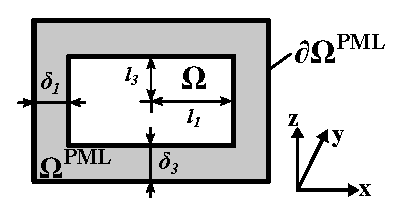
\includegraphics[scale=1.25]{research-2/info_2d/info_2d_2.eps}
	\caption{геометрические характеристики PML-слоя}
	\label{fig:res2:info_2d}
\end{figure}

Вычислительные эксперименты проводились следующим образом: последовательно варьировался каждый из параметров PML-слоя: толщина слоя в $k$-м направлении $\delta_k$, где $k = \begin{smallmatrix}x\\1\end{smallmatrix},\begin{smallmatrix}y\\2\end{smallmatrix},\begin{smallmatrix}z\\3\end{smallmatrix}$, расстояние от центра области до внутренних границ слоя $l_k$, коэффициент комплексного растяжения координат $\chi$~(\ref{eq:pml_s}), оставшиеся параметры фиксировались, что позволило определить параметры, оказывающие наибольшее влияние на характеристики PML-слоя.

\begin{figure}[H]
	\centering
	% trim=left bottom right top
	\subfloat[][]{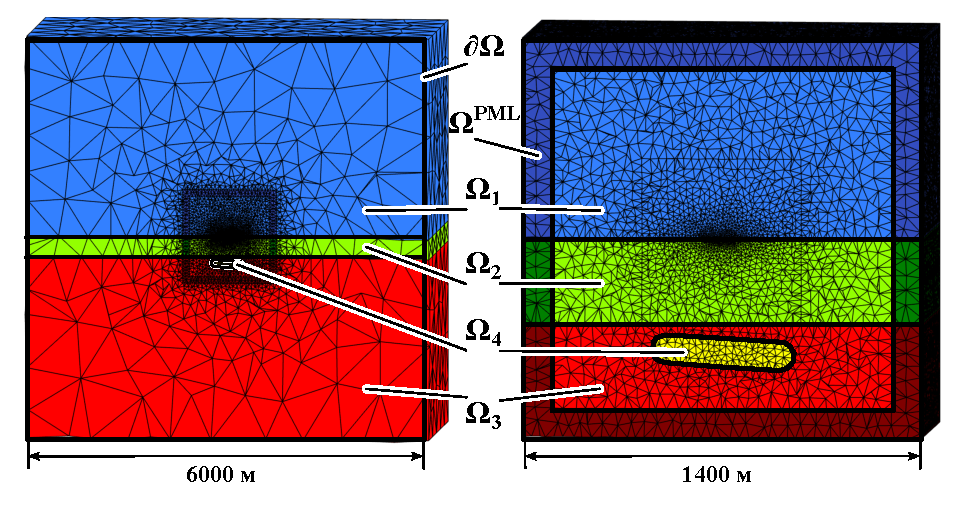
\includegraphics[trim=0mm 0mm 79.2mm 0mm,clip,scale=1.1]{research-2/meshes/meshes_color.eps}\label{fig:res2:meshes_a}}
	\subfloat[][]{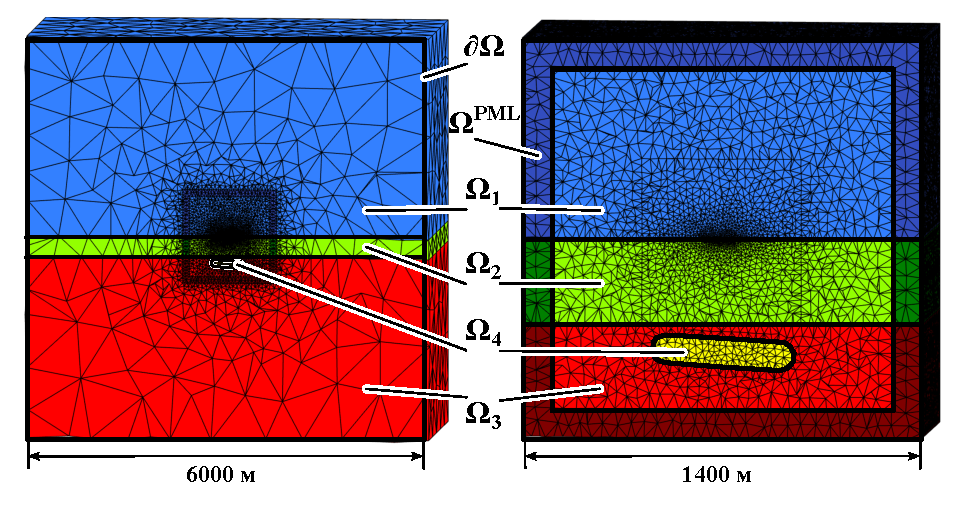
\includegraphics[trim=79.2mm 0mm 0mm 0mm,clip,scale=1.1]{research-2/meshes/meshes_color.eps}\label{fig:res2:meshes_b}}
	\caption{конечноэлементные сетки: (а) <<большой бак>> и (б) PML-слой}
	\label{fig:res2:meshes}
\end{figure}

Фрагменты тетраэдральных конечноэлементных сеток с <<большим баком>> и с PML-слоем приведены на рисунках \ref{fig:res2:meshes_a} и \ref{fig:res2:meshes_b}.

В этом исследовании будем пользоваться базисными функциями первого полного порядка.

\subsubsection{Описание расчётной области}
Расчётная область показана на рисунке \ref{fig:res2:area}, где $\Omega_1$ -- воздух ($\sigma=10^{-6}$ См/м, $\mu=\mu_0$, $\varepsilon=\varepsilon_0$); $\Omega_2$ -- морская вода ($\sigma=3.3$ См/м, $\mu=\mu_0$, $\varepsilon=\varepsilon_0$); $\Omega_3$ -- грунт ($\sigma=0.2$ См/м, $\mu=\mu_0$, $\varepsilon=\varepsilon_0$); $\Omega_4$ -- углеводороды ($\sigma=10^{-2}$~См/м, $\mu=\mu_0$, $\varepsilon=\varepsilon_0$); $L_1$, $L_2$ и $L_3$ -- размеры области моделирования по осям $x$, $y$ и $z$ соответственно; $L_1 = L_2 = L_3 = 6000$~м; $h_1=300$~м -- толщина $\Omega_2$; $l_1=400$~м, $h_3=100$~м, $h_2=100$~м -- длина, толщина и глубина объекта $\Omega_4$ соответственно.

\begin{figure}[H]
	\centering
	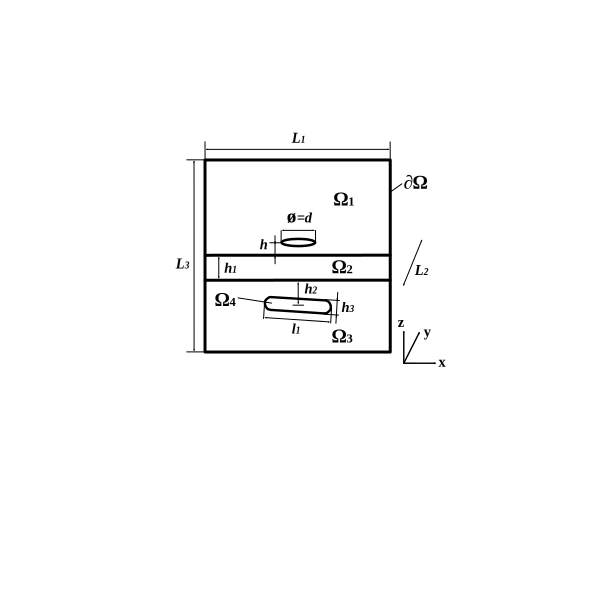
\includegraphics[scale=1.5]{research-2/area_3layers/area_3layers_3.eps}
	\caption{расчётная область}
	\label{fig:res2:area}
\end{figure}

Объект $\Omega_4$ представляет собой скруглённый прямоугольный параллелепипед с двумя равными сторонами, наклонённый под углом $5^{\circ}$. В качестве источника электрического поля выступает петля диаметром $d = 100$~м с током частотой $1$~Гц, расположенная в воздухе на расстоянии $h = 5$~м от границы раздела сред воздух-вода. Также рассматривается случай, когда петля расположена в воде ($h = -5$~м).

Выделим внутри области c условием <<большого бака>> и области, на границе которой задан PML-слой, подобласть $\Omega'$ размером $1000 \times 1000 \times 1000$~м${}^3$. Для этой подобласти в данном исследовании будем оценивать разность в норме $\mathbb{L}^2$ между действительными компонентами $\mathbf{E}_y$ векторов решений $\mathbf{E}_y^{\text{бак}}$ и $\mathbf{E}_y^{\text{PML}}$, полученных с применением <<большого бака>> и PML-слоя соответственно.

\subsubsection{Варьирование коэффициентов растяжения}
Зафиксируем $\delta_k = 100$~м, $l_k = 600$~м, $m = 3$, $h = 5$~м и будем варьировать коэффициент комплексного растяжения координат $\chi$. Размер получаемой СЛАУ для <<большого бака>> -- 653814, с PML-слоем -- 616180. Результаты приведены в таблице \ref{tab:res2:chi_5}. Для случая $h= -5$~м размер получаемой СЛАУ для <<большого бака>> -- 652396, с PML-слоем -- 614504. Результаты приведены в таблице \ref{tab:res2:chi_m5}.
\begin{table}[H]
	\caption{варьирование коэффициентов растяжения при $h= 5$~м}
	\label{tab:res2:chi_5}
	\begin{spacing}{1.2}
	\setlength{\parskip}{0pt}
	\fontsize{12}{14}\selectfont
	\begin{tabularx}{\textwidth}{|C{0.65}|C{0.65}|C{0.65}|C{0.65}|C{0.65}|C{0.65}|C{3.1}|C{1}|C{1}|}
		\rowcolor[gray]{.9} \hline $\Re(\chi)$ в $\Omega_1$ & $\Im(\chi)$ в $\Omega_1$ & $\Re(\chi)$ в $\Omega_2$ & $\Im(\chi)$ в $\Omega_2$ & $\Re(\chi)$ в $\Omega_3$ & $\Im(\chi)$ в $\Omega_3$ & \raisebox{-0.8em}{$\smash{\displaystyle \frac{\lVert \Re(\mathbf{E}_y^{\text{бак}}) - \Re(\mathbf{E}_y^{\text{PML}})\rVert}{\lVert \Re(\mathbf{E}_y^{\text{бак}})\rVert}}$} & Время, бак & Время, PML \\[0.2em]
		\hline 3 & 0 & 1 & 5 & 3 & 1 & 0.106636 & \multirow{4}{*}{650} & 592 \\
		\cline{1-7}\cline{9-9} 3 & 1 & 0 & 6 & 2 & 1 & 0.0925 & & 599 \\
		\cline{1-7}\cline{9-9} 4 & 0 & 1 & 5 & 3 & 1 & 0.0947 & & 731 \\
		\cline{1-7}\cline{9-9} 4 & 1 & 0 & 6 & 2 & 1 & 0.0910 & & 591 \\
		\hline
	\end{tabularx}
	\end{spacing}
\end{table}

\begin{table}[H]
	\caption{варьирование коэффициентов растяжения при $h= -5$~м}
	\label{tab:res2:chi_m5}
	\begin{spacing}{1.2}
	\setlength{\parskip}{0pt}
	\fontsize{12}{14}\selectfont
	\begin{tabularx}{\textwidth}{|C{0.65}|C{0.65}|C{0.65}|C{0.65}|C{0.65}|C{0.65}|C{3.1}|C{1}|C{1}|}
		\rowcolor[gray]{.9} \hline $\Re(\chi)$ в $\Omega_1$ & $\Im(\chi)$ в $\Omega_1$ & $\Re(\chi)$ в $\Omega_2$ & $\Im(\chi)$ в $\Omega_2$ & $\Re(\chi)$ в $\Omega_3$ & $\Im(\chi)$ в $\Omega_3$ & \raisebox{-0.8em}{$\smash{\displaystyle \frac{\lVert \Re(\mathbf{E}_y^{\text{бак}}) - \Re(\mathbf{E}_y^{\text{PML}})\rVert}{\lVert \Re(\mathbf{E}_y^{\text{бак}})\rVert}}$} & Время, бак & Время, PML \\[0.2em]
		\hline 4 & 0 & 1 & 5 & 3 & 1 & 0.0929047 & \multirow{4}{*}{309} & 344 \\
		\cline{1-7}\cline{9-9} 4 & 0 & 1 & 6 & 3 & 1 & 0.0870 & & 294 \\
		\cline{1-7}\cline{9-9} 4 & 0 & 1 & 6 & 3 & 2 & 0.0809 & & 253 \\
		\cline{1-7}\cline{9-9} 4 & 1 & 1 & 6 & 3 & 2 & 0.0658 & & 306 \\
		\hline
	\end{tabularx}
	\end{spacing}
\end{table}

\subsubsection{Варьирование толщины PML-слоя}
Зафиксируем $\chi_{\Omega_1} = (4, 1)$, $\chi_{\Omega_2} = (0, 6)$, $\chi_{\Omega_3} = (2, 1)$, $l_k = 600$~м, $m = 3$, $h = 5$~м и будем варьировать толщину PML-слоя $\delta_k$. Результаты приведены в таблице \ref{tab:res2:delta_5}. Для случая $h= -5$~м выберем $\chi_{\Omega_1} = (4, 0)$, $\chi_{\Omega_2} = (1, 6)$, $\chi_{\Omega_3} = (3, 2)$. Результаты приведены в таблице \ref{tab:res2:delta_m5}.

\begin{table}[H]
	\caption{варьирование толщины PML-слоя при $h= 5$~м}
	\label{tab:res2:delta_5}
	\begin{spacing}{1.2}
	\setlength{\parskip}{0pt}
	\fontsize{12}{14}\selectfont
	\begin{tabularx}{\textwidth}{|C{0.4}|C{2.2}|C{0.8}|C{0.8}|C{0.9}|C{0.9}|}
		\rowcolor[gray]{.9} \hline \raisebox{-0.8em}[0.8em]{$\smash{\displaystyle \delta_k}$} & \raisebox{-0.8em}[0.8em]{$\smash{\displaystyle \frac{\lVert \Re(\mathbf{E}_y^{\text{бак}}) - \Re(\mathbf{E}_y^{\text{PML}})\rVert}{\lVert \Re(\mathbf{E}_y^{\text{бак}})\rVert}}$} & Время, бак & Время, PML & Размер СЛАУ, бак & Размер СЛАУ, PML \\[0.2em]
		\hline 80 & 0.1199 & 673 & 1289 & 659858 & 618128 \\
		\hline 100 & 0.0910 & 650 & 591 & 653814 & 616180 \\
		\hline 120 & 0.0784 & 609 & 1142 & 654354 & 617324 \\
		\hline
	\end{tabularx}
	\end{spacing}
\end{table}

\begin{table}[H]
	\caption{варьирование толщины PML-слоя при $h= -5$~м}
	\label{tab:res2:delta_m5}
	\begin{spacing}{1.2}
	\setlength{\parskip}{0pt}
	\fontsize{12}{14}\selectfont
	\begin{tabularx}{\textwidth}{|C{0.4}|C{2.2}|C{0.8}|C{0.8}|C{0.9}|C{0.9}|}
		\rowcolor[gray]{.9} \hline \raisebox{-0.8em}[0.8em]{$\smash{\displaystyle \delta_k}$} & \raisebox{-0.8em}[0.8em]{$\smash{\displaystyle \frac{\lVert \Re(\mathbf{E}_y^{\text{бак}}) - \Re(\mathbf{E}_y^{\text{PML}})\rVert}{\lVert \Re(\mathbf{E}_y^{\text{бак}})\rVert}}$} & Время, бак & Время, PML & Размер СЛАУ, бак & Размер СЛАУ, PML \\[0.2em]
		\hline 80 & 0.1201 & 359 & 297 & 652312 & 614822 \\
		\hline 100 & 0.0809 & 309 & 253 & 652396 & 614504 \\
		\hline 120 & 0.0623 & 250 & 859 & 652422 & 615394\\
		\hline
	\end{tabularx}
	\end{spacing}
\end{table}

\subsubsection{Варьирование размера области, на границе которой вводится PML-слой}
Зафиксируем $\chi_{\Omega_1} = (4, 1)$, $\chi_{\Omega_2} = (0, 6)$, $\chi_{\Omega_3} = (2, 1)$, $\delta_k = 100$~м, $m = 3$, $h = 5$~м и будем варьировать $l_k$ -- размер области, на границе которой вводится PML-слой. Результаты приведены в таблице \ref{tab:res2:l_5}. Для случая $h= -5$~м выберем $\chi_{\Omega_1} = (4, 0)$, $\chi_{\Omega_2} = (1, 6)$, $\chi_{\Omega_3} = (3, 2)$. Результаты приведены в таблице \ref{tab:res2:l_m5}.

\begin{table}[H]
	\caption{варьирование размера области, на границе которой вводится PML-слой, при $h= 5$~м}
	\label{tab:res2:l_5}
	\begin{spacing}{1.2}
	\setlength{\parskip}{0pt}
	\fontsize{12}{14}\selectfont
	\begin{tabularx}{\textwidth}{|C{0.4}|C{2.2}|C{0.8}|C{0.8}|C{0.9}|C{0.9}|}
		\rowcolor[gray]{.9} \hline \raisebox{-0.8em}[0.8em]{$\smash{\displaystyle l_k}$} & \raisebox{-0.8em}[0.8em]{$\smash{\displaystyle \frac{\lVert \Re(\mathbf{E}_y^{\text{бак}}) - \Re(\mathbf{E}_y^{\text{PML}})\rVert}{\lVert \Re(\mathbf{E}_y^{\text{бак}})\rVert}}$} & Время, бак & Время, PML & Размер СЛАУ, бак & Размер СЛАУ, PML \\[0.2em]
		\hline 500 & 0.187456 & 628 & 587 & 659130 & 621390 \\
		\hline 600 & 0.0909998 & 650 & 591 & 652396 & 614504 \\
		\hline 800 & 0.0440642 & 718 & 658 & 794310 & 744856 \\
		\hline
	\end{tabularx}
	\end{spacing}
\end{table}

\begin{table}[H]
	\caption{варьирование размера области, на границе которой вводится PML-слой, при $h= -5$~м}
	\label{tab:res2:l_m5}
	\begin{spacing}{1.2}
	\setlength{\parskip}{0pt}
	\fontsize{12}{14}\selectfont
	\begin{tabularx}{\textwidth}{|C{0.4}|C{2.2}|C{0.8}|C{0.8}|C{0.9}|C{0.9}|}
		\rowcolor[gray]{.9} \hline \raisebox{-0.8em}[0.8em]{$\smash{\displaystyle l_k}$} & \raisebox{-0.8em}[0.8em]{$\smash{\displaystyle \frac{\lVert \Re(\mathbf{E}_y^{\text{бак}}) - \Re(\mathbf{E}_y^{\text{PML}})\rVert}{\lVert \Re(\mathbf{E}_y^{\text{бак}})\rVert}}$} & Время, бак & Время, PML & Размер СЛАУ, бак & Размер СЛАУ, PML \\[0.2em]
		\hline 500 & 0.1751746 & 317 & 238 & 659814 & 621390 \\
		\hline 600 & 0.0809429 & 309 & 253 & 652396 & 614504 \\
		\hline 800 & 0.0348019 & 357 & 329 & 793272 & 743780 \\
		\hline
	\end{tabularx}
	\end{spacing}
\end{table}

\subsubsection{Проверка выполнения условий на контактных границах}
Проверим, что в случае независимого варьирования коэффициентов комплексного растяжения координат $\chi$, на границе двух соседних PML-слоёв с различными характеристиками не нарушаются условия на контактных границах (\ref{eq:maxwell:tangent_E})-(\ref{eq:maxwell:normal_D}). Для этого рассмотрим напряжённость электрического поля $\mathbf{E}$ вдоль линии $x = 650$, $y = 0$, $z = [-0.005, 0.005]$ (середина PML-слоя по $x$-направлению):
\begin{figure}[H]
	\centering
	\includegraphics[scale=1]{research-2/650/ExR.eps}
	\includegraphics[scale=1]{research-2/650/ExI.eps}
	\includegraphics[scale=1]{research-2/650/EyR.eps}
	\includegraphics[scale=1]{research-2/650/EyI.eps}
	\includegraphics[scale=1]{research-2/650/EzR.eps}
	\includegraphics[scale=1]{research-2/650/EzI.eps}
	\caption{графики компонент электрического поля на контактных границах}
	\label{fig:res2:650_3}
\end{figure}

Как видно из графиков на рисунке \ref{fig:res2:650_3}, разрывна только нормальная компонента $\mathbf{E}_z$, следовательно, условия (\ref{eq:maxwell:tangent_E})-(\ref{eq:maxwell:normal_D}) выполнены.

\subsubsection{Графическое представление результатов}
Рассмотрим результаты, полученные при параметрах $h=5$~м, $\chi_{\Omega_1} = (4, 0)$, $\chi_{\Omega_2} = (1, 6)$, $\chi_{\Omega_2} = (3, 2)$, $m=3$, $l_k = 600$~м и $\delta_k = 100$~м. На рисунках \ref{fig:res2:field_sca} и \ref{fig:res2:field_vec} показаны картины электрического поля в сечении плоскостью $z = -10$~м. На рисунках \ref{fig:res2:field_sca_a} и \ref{fig:res2:field_vec_a} представлено решение с PML-слоем; \ref{fig:res2:field_sca_b} и \ref{fig:res2:field_vec_b} -- решение с <<большим баком>>.

\begin{figure}[H]
	\centering
	\subfloat[][]{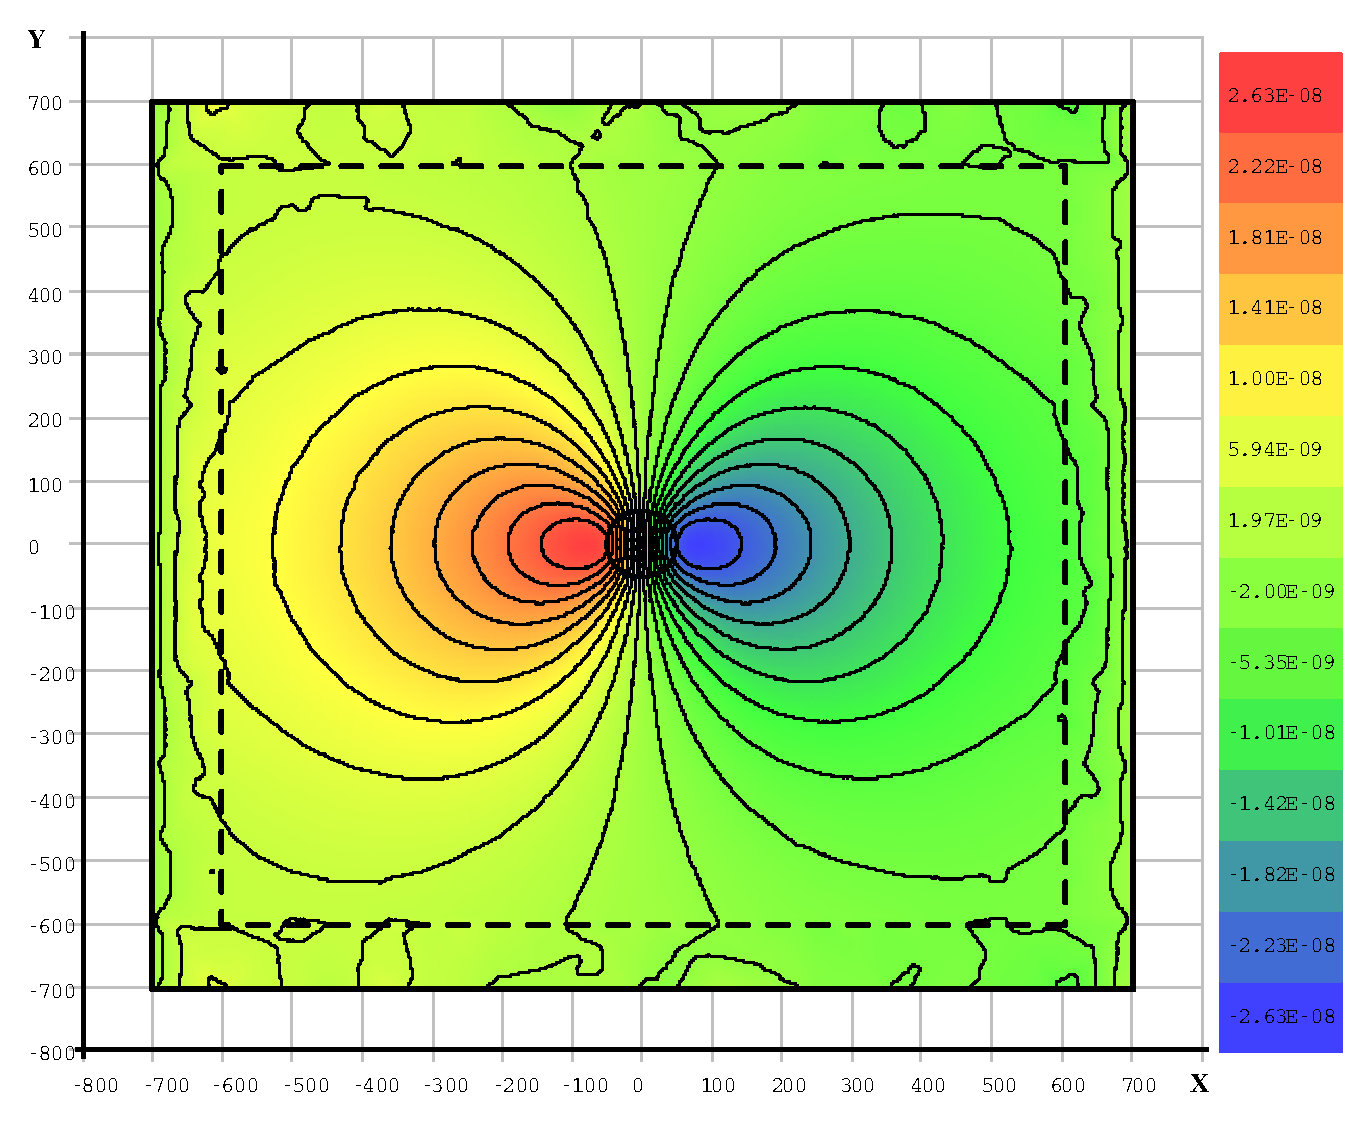
\includegraphics[scale=0.35]{research-2/field/airloop/pml/airloop_pml_z=-10_EyR.eps}\label{fig:res2:field_sca_a}}
	~~
	\subfloat[][]{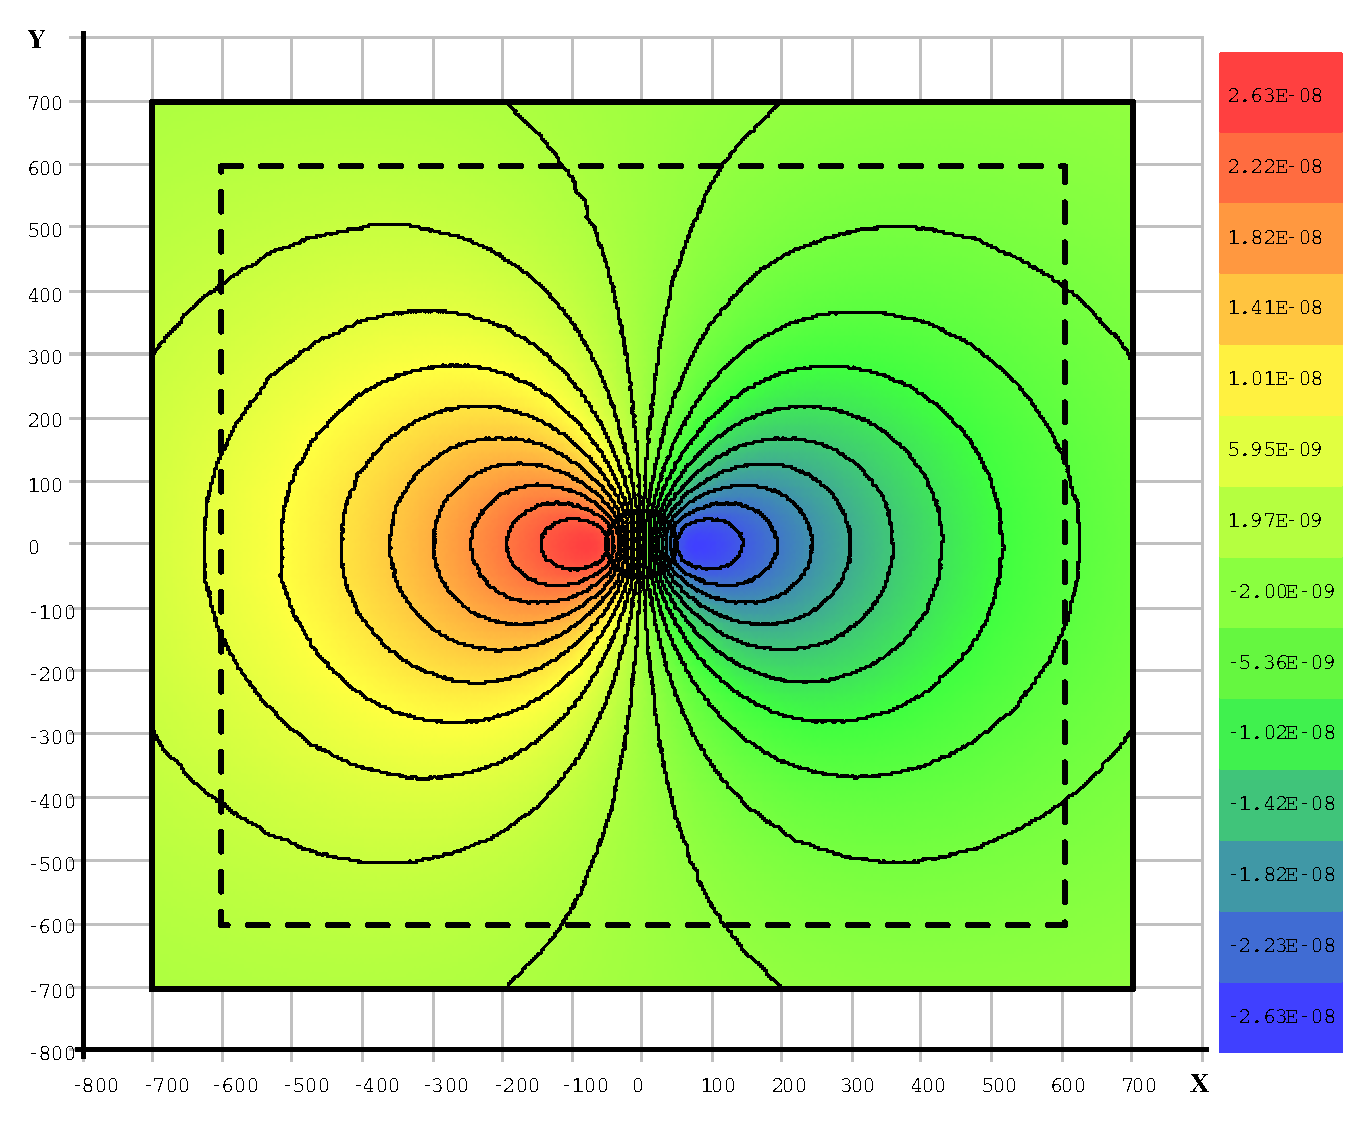
\includegraphics[scale=0.35]{research-2/field/airloop/std/airloop_std_z=-10_EyR.eps}\label{fig:res2:field_sca_b}}
	\caption{$\Re(\mathbf{E}_y)$}
	\label{fig:res2:field_sca}
\end{figure}

\vspace{-0.8cm}

\begin{figure}[H]
	\centering
	\subfloat[][]{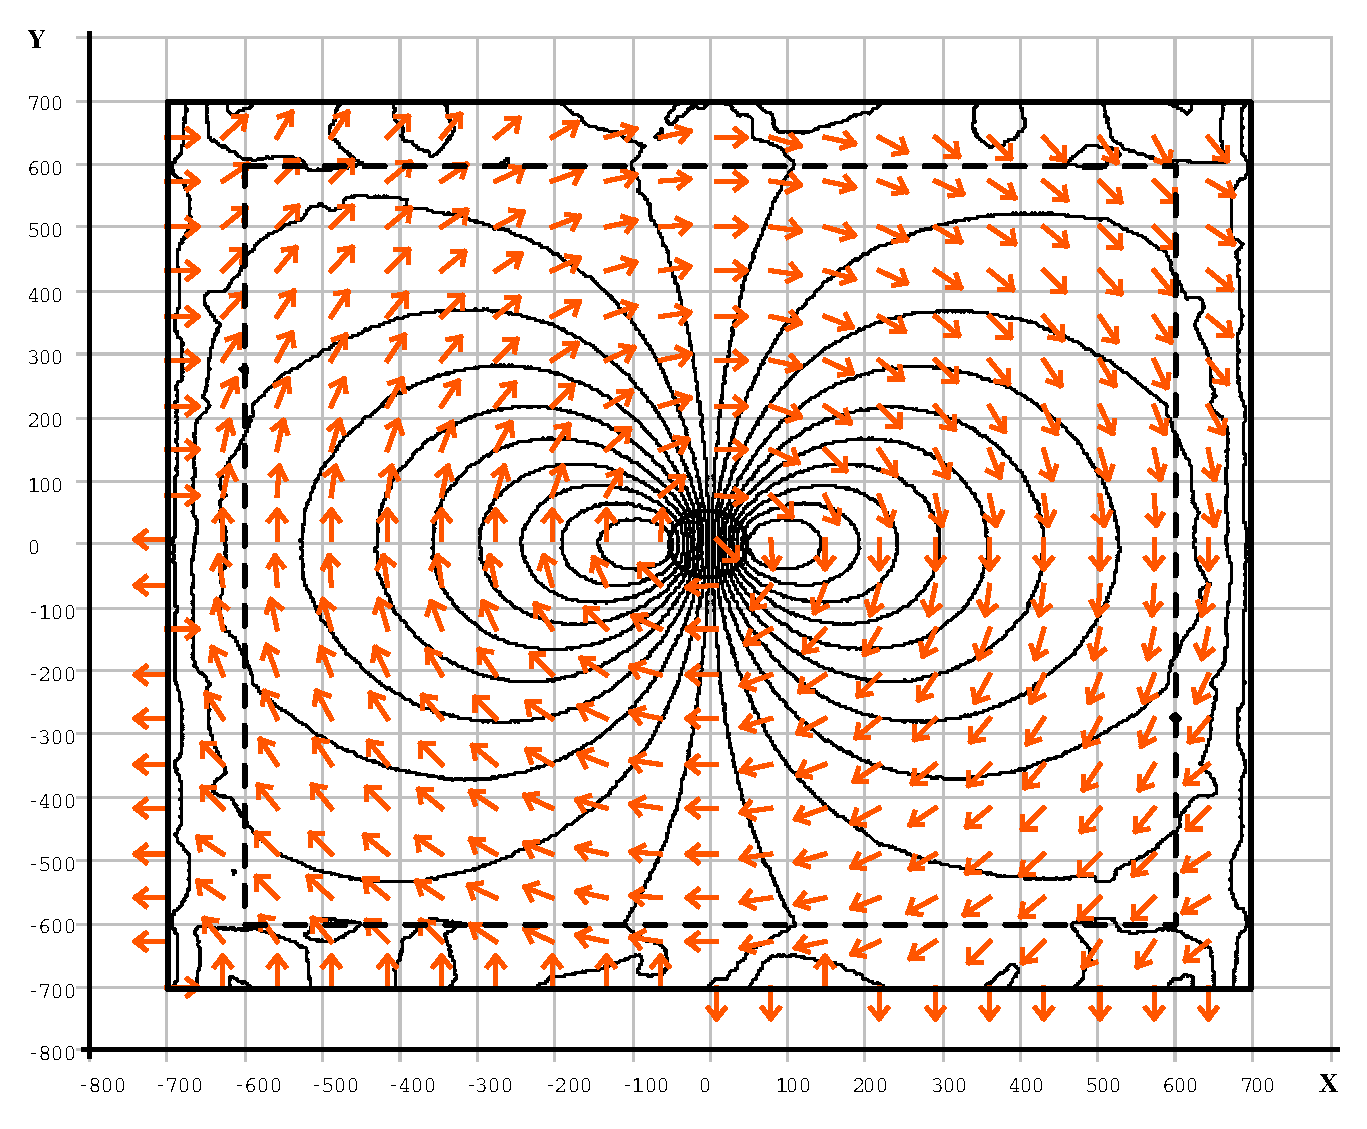
\includegraphics[scale=0.35]{research-2/field/airloop/pml/airloop_pml_z=-10_EyR_vec.eps}\label{fig:res2:field_vec_a}}
	~~
	\subfloat[][]{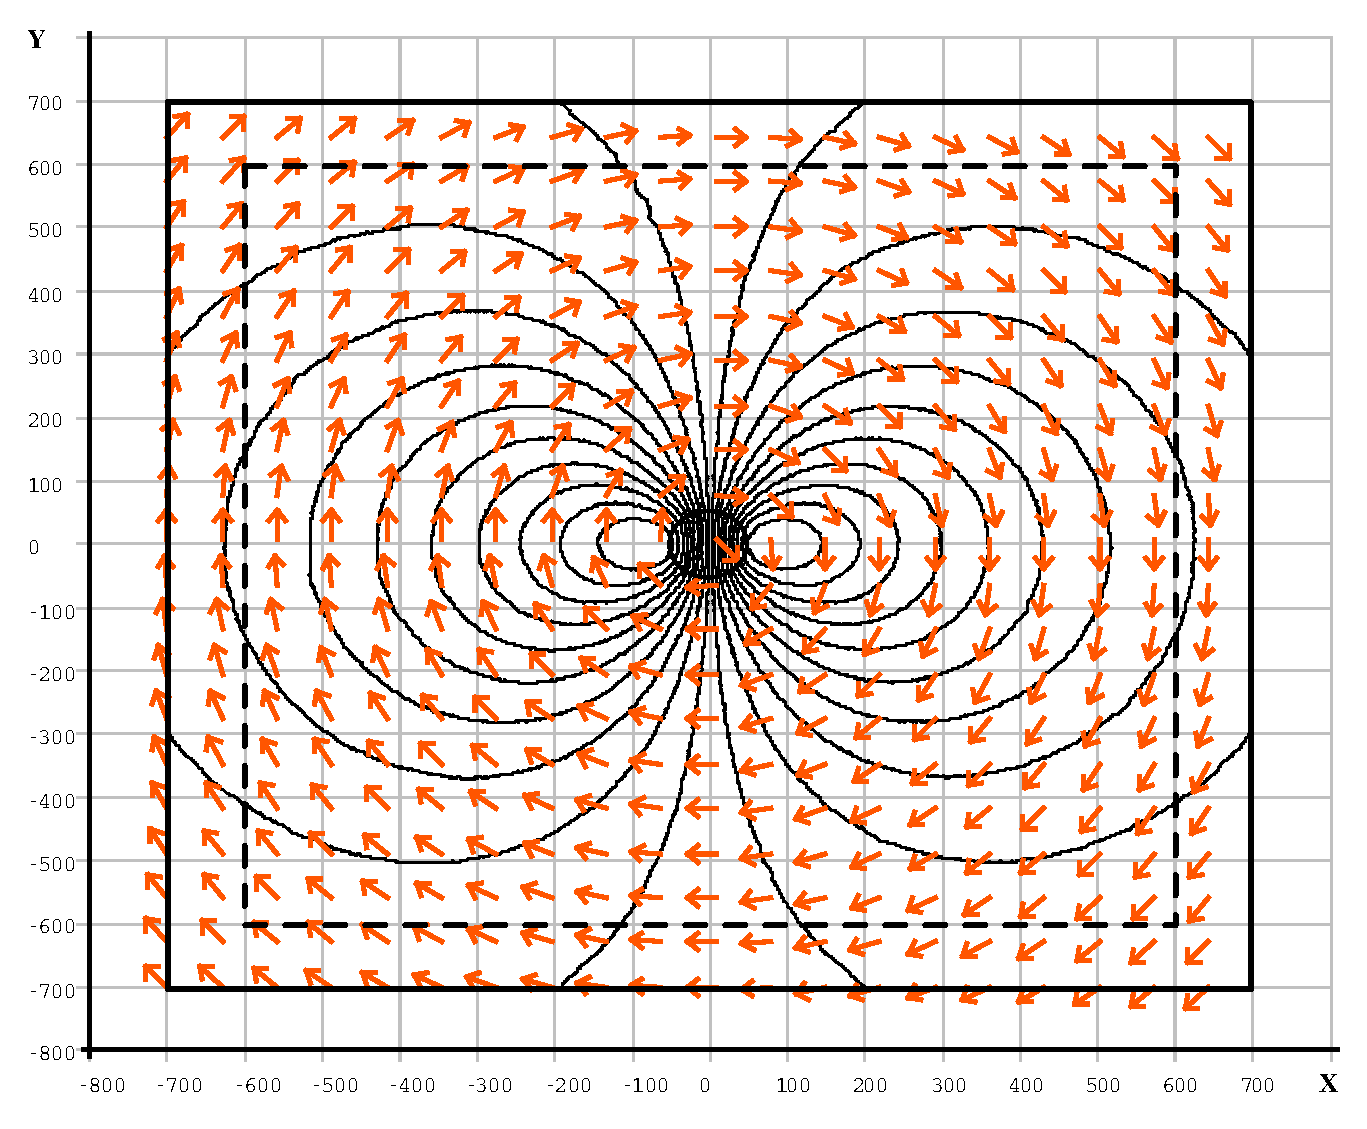
\includegraphics[scale=0.35]{research-2/field/airloop/std/airloop_std_z=-10_EyR_vec.eps}\label{fig:res2:field_vec_b}}
	\caption{изолинии $\Re(\mathbf{E}_y)$ и векторы $\left( \Re(\mathbf{E}_x) , \Re(\mathbf{E}_y) \right)^T$}
	\label{fig:res2:field_vec}
\end{figure}

На рисунке \ref{fig:res2:field_y0} показаны картины электрического поля в сечении плоскостью $y=0$. На рисунках \ref{fig:res2:field_y0_a} и \ref{fig:res2:field_y0_b} представлено решение с PML-слоем и решение с <<большим баком>> соответственно.

\begin{figure}[H]
	\centering
	\subfloat[][]{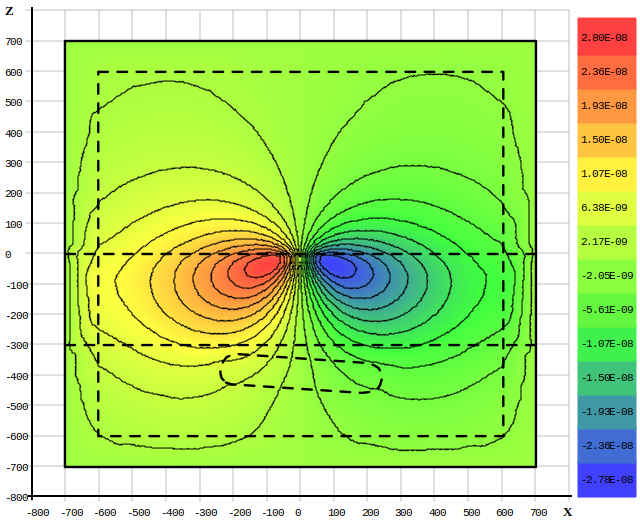
\includegraphics[scale=0.35]{research-2/field/airloop/pml/airloop_pml_y=0_EyR.eps}\label{fig:res2:field_y0_a}}
	~~
	\subfloat[][]{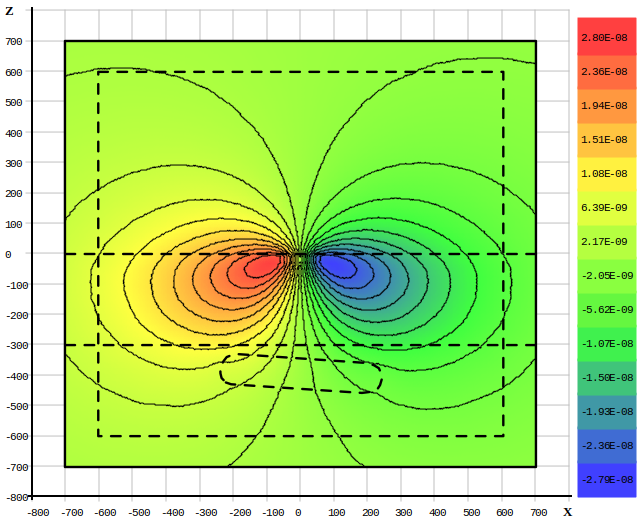
\includegraphics[scale=0.35]{research-2/field/airloop/std/airloop_std_y=0_EyR.eps}\label{fig:res2:field_y0_b}}
	\caption{$\Re(\mathbf{E}_y)$}
	\label{fig:res2:field_y0}
\end{figure}

% =============================================================================

\subsubsection{Анализ целесообразности применения PML-слоя}
Наибольшее влияние на точность получаемого решения при введении PML-слоя оказывают коэффициент комплексного растяжения координат $\chi$ и $l$ -- размер области, на границе которой вводится PML-слой. При увеличении размера внутренней области ожидаемо увеличивается размер СЛАУ, поэтому этот параметр при решении реальных задач следует не варьировать, а выбрать как некоторое ограничение. Таким образом, в первую очередь стоит проводить поиск оптимального значения именно для коэффициента растяжения $\chi$. Выбор толщины PML-слоя влияет на точность решения незначительно, поэтому достаточно лишь убедиться, что она выбрана в подходящих для задачи пределах -- не слишком большой и не слишком маленькой.

В рассмотренном виде применение PML-слоя для сокращения области моделирования задач низкочастотной морской геоэлектрики незначительно уменьшает размерность СЛАУ и, в большинстве случаев, не приводит к существенному сокращению времени решения задачи. Одной из причин этого может быть то, что основное растяжение приходится на вещественные компоненты координат. Это приводит к значительной <<вытянутости>> тетраэдров внутри PML-слоя и, как следствие, сильному ухудшению свойств матрицы СЛАУ и увеличению времени решения. Параллелепипедальные конечные элементы лишены подобного недостатка, поэтому для них можно проводить комплексное растяжение в гораздо больших диапазонах. Однако, такие элементы не подходят для аппроксимации сколь-либо сложных областей. Для использования в одной сетке и тетраэдральных, и параллелепипедальных конечных элементов можно применять специальные переходные элементы~\citep{extra_elements1,extra_elements2}, либо воспользоваться неконформными методами~\citep{dg1,dg2,dg3,mortar1,mortar2}.

% =============================================================================

\subsection{Задача, приближенная к реальной}
В этом исследовании рассмотрим поведение электрического поля при различном расположении источника этого поля относительно объекта, скрытого в грунте. Различное положение источника обеспечивается за счёт <<протаскивания>> его на некотором расстоянии от морского дна.

В этом исследовании будем пользоваться базисными функциями второго полного порядка.

\subsubsection{Описание расчётной области}
Расчётная область показана на рисунке \ref{fig:res3:area}, где $\Omega_1$ -- воздух ($\sigma=10^{-6}$ См/м, $\mu=\mu_0$, $\varepsilon=\varepsilon_0$); $\Omega_2$ -- морская вода ($\sigma=3.3$ См/м, $\mu=\mu_0$, $\varepsilon=\varepsilon_0$); $\Omega_3$ -- грунт ($\sigma=0.2$ См/м, $\mu=\mu_0$, $\varepsilon=\varepsilon_0$); $\Omega_4$ -- углеводороды ($\sigma=10^{-2}$~См/м, $\mu=\mu_0$, $\varepsilon=\varepsilon_0$); $L_1$, $L_2$ и $L_3$ -- размеры области моделирования по осям $x$, $y$ и $z$ соответственно; $L_1 = L_2 = L_3 = 6000$~м; $h_1=600$~м -- толщина $\Omega_2$; $l_1=400$~м, $h_3=75$~м, $h_2=120$~м -- длина, толщина и глубина объекта $\Omega_4$ соответственно.

В качестве источника электрического поля выступает петля диаметром $d=100$ м с током частотой 1 Гц, расположенная в воде на расстоянии $h=590$ м от границы раздела сред воздух-вода (в 10 метрах над поверхностью грунта). Объект $\Omega_4$
%, как и в предыдущих исследованиях, 
представляет собой скруглённый прямоугольный параллелепипед с двумя равными сторонами, наклонённый под углом $5^{\circ}$.

В этой области рассмотрим электрическое поле при различных смещениях объекта относительно источника ($l_2=-300$, $-200$, $-100$ и $0$ м), а также сравним с электрическим полем в случае проводящего объекта ($\sigma=10^2$ См/м).

\begin{figure}[H]
	\centering
	\includegraphics[scale=0.7]{research-3/area/area_3layers_shift_3.eps}
	\caption{расчётная область}
	\label{fig:res3:area}
\end{figure}

\subsubsection{Конечноэлементная сетка}
Фрагмент $x \in [-600,0]$, $y \in [-600,600]$ $z \in [-1000,600]$ одной из конечноэлементных сеток, использованных для проведения исследования, представлен на рисунке \ref{fig:res3:mesh}.

\begin{figure}[H]
	\centering
	% trim=left bottom right top
	\includegraphics[trim=390mm 20mm 5mm 195mm,clip,scale=0.5]{research-3/mesh/mesh.png}
	\caption{фрагмент конечноэлементной сетки}
	\label{fig:res3:mesh}
\end{figure}

\subsubsection{Результаты вычислительного эксперимента}
Рассмотрим результаты для проводящего и непроводящего объекта при различных его смещениях относительно источника ($l_2=-300$, $-200$, $-100$ и $0$ м). На рисунках \ref{fig:res3:0_EyR}-\ref{fig:res3:0_vec} показано графическое представление напряжённости электрического поля $\mathbf{E}$ при $l_2=0$ в сечении $y=0$, на рисунках \ref{fig:res3:0_EyR_a} и \ref{fig:res3:0_vec_a} -- для объекта с $\sigma=10^{-2}$~См/м, на рисунках \ref{fig:res3:0_EyR_b} и \ref{fig:res3:0_vec_b} -- для объекта с $\sigma=10^{2}$~См/м.

%\begin{spacing}{1.0}
%\setlength{\parskip}{0pt}

\begin{figure}[H]
	\centering
	\subfloat[][]{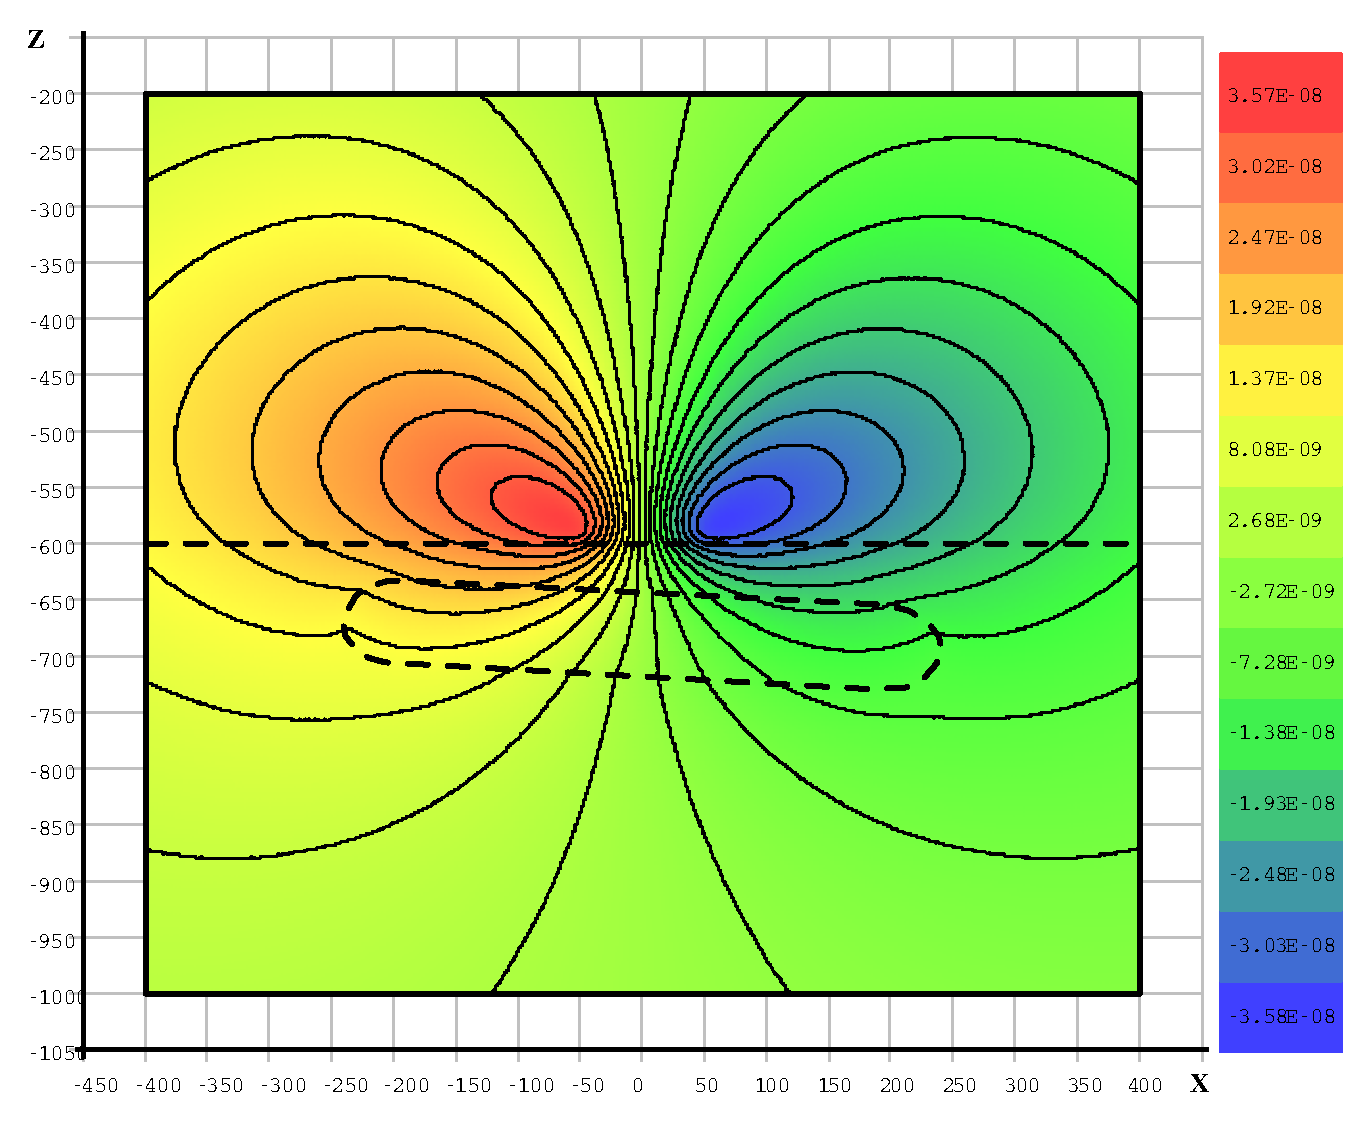
\includegraphics[scale=0.36]{research-3/fields/images/0/0_no_y=0_EyR.eps}\label{fig:res3:0_EyR_a}}
	\text{~~}
	\subfloat[][]{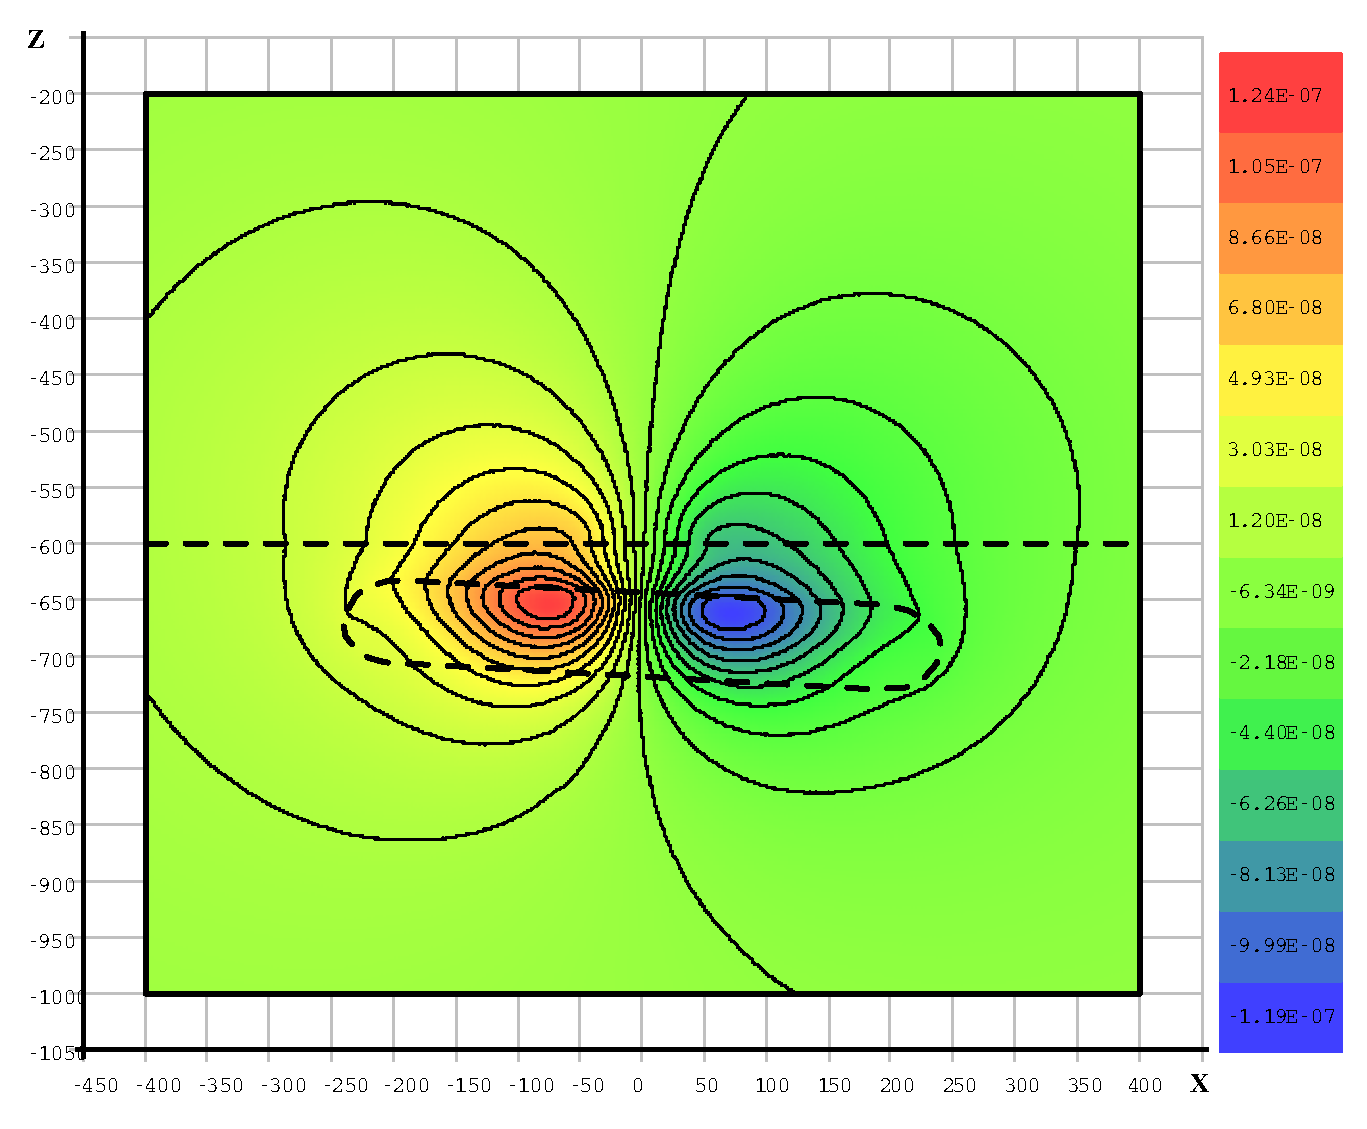
\includegraphics[scale=0.36]{research-3/fields/images/0/0_yes_y=0_EyR.eps}\label{fig:res3:0_EyR_b}}
	\caption{$\Re(\mathbf{E}_y)$ при $l_2=0$}
	\label{fig:res3:0_EyR}
\end{figure}

%\vspace{-0.8cm}

\begin{figure}[H]
	\centering
	\subfloat[][]{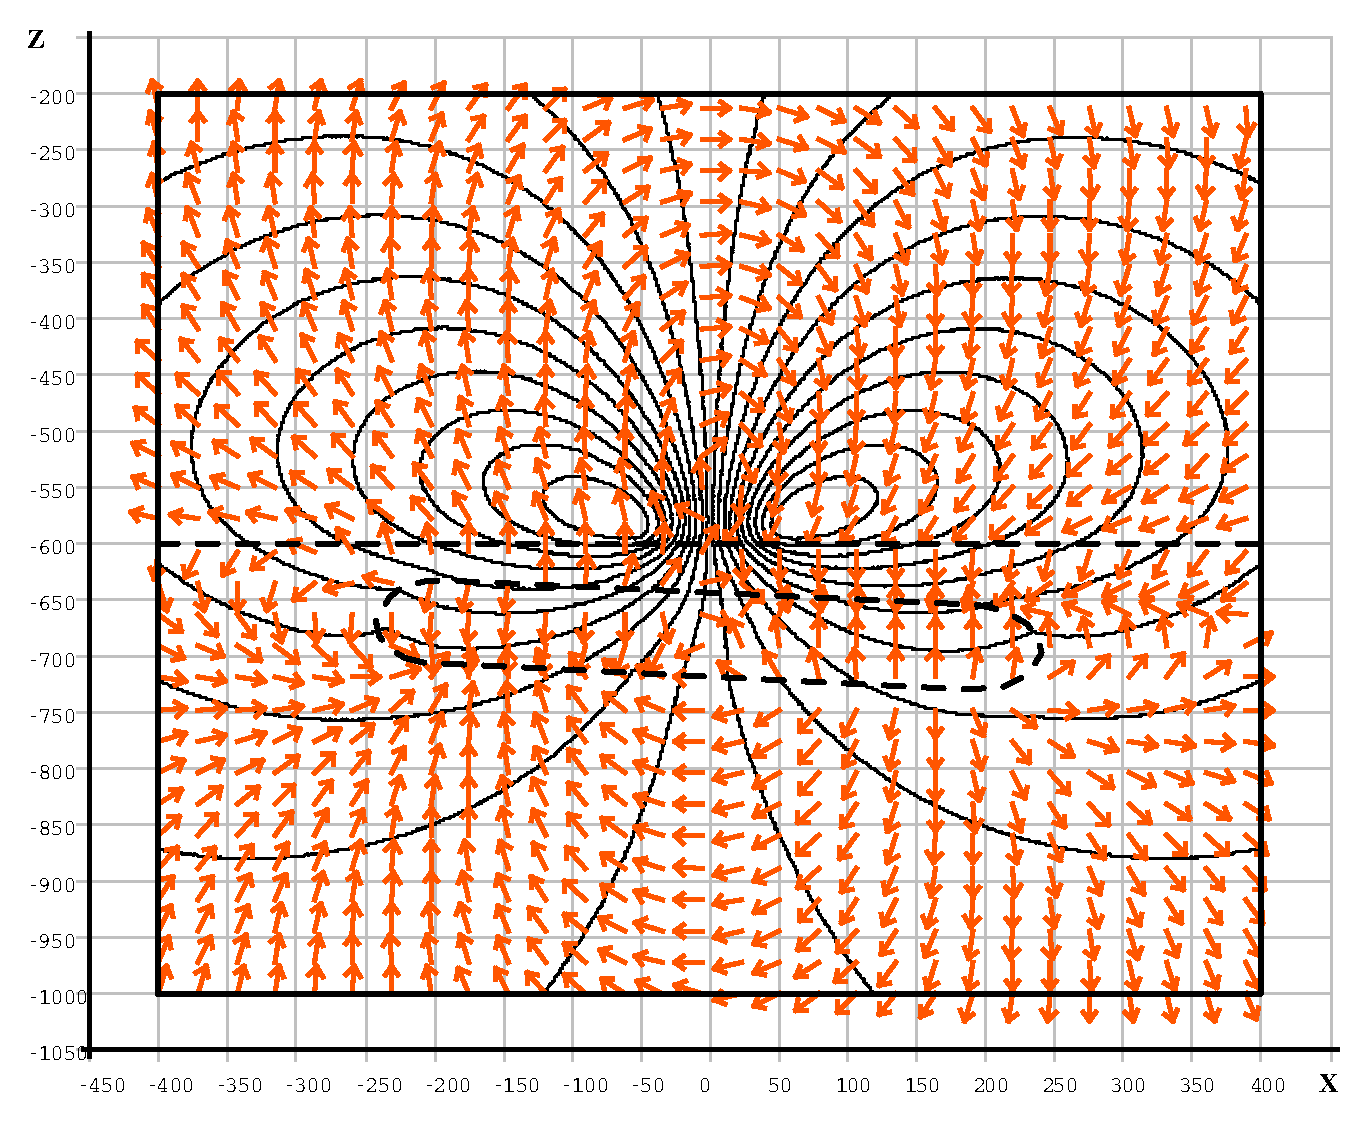
\includegraphics[scale=0.36]{research-3/fields/images/0/0_no_y=0_vec.eps}\label{fig:res3:0_vec_a}}
	\text{~~}
	\subfloat[][]{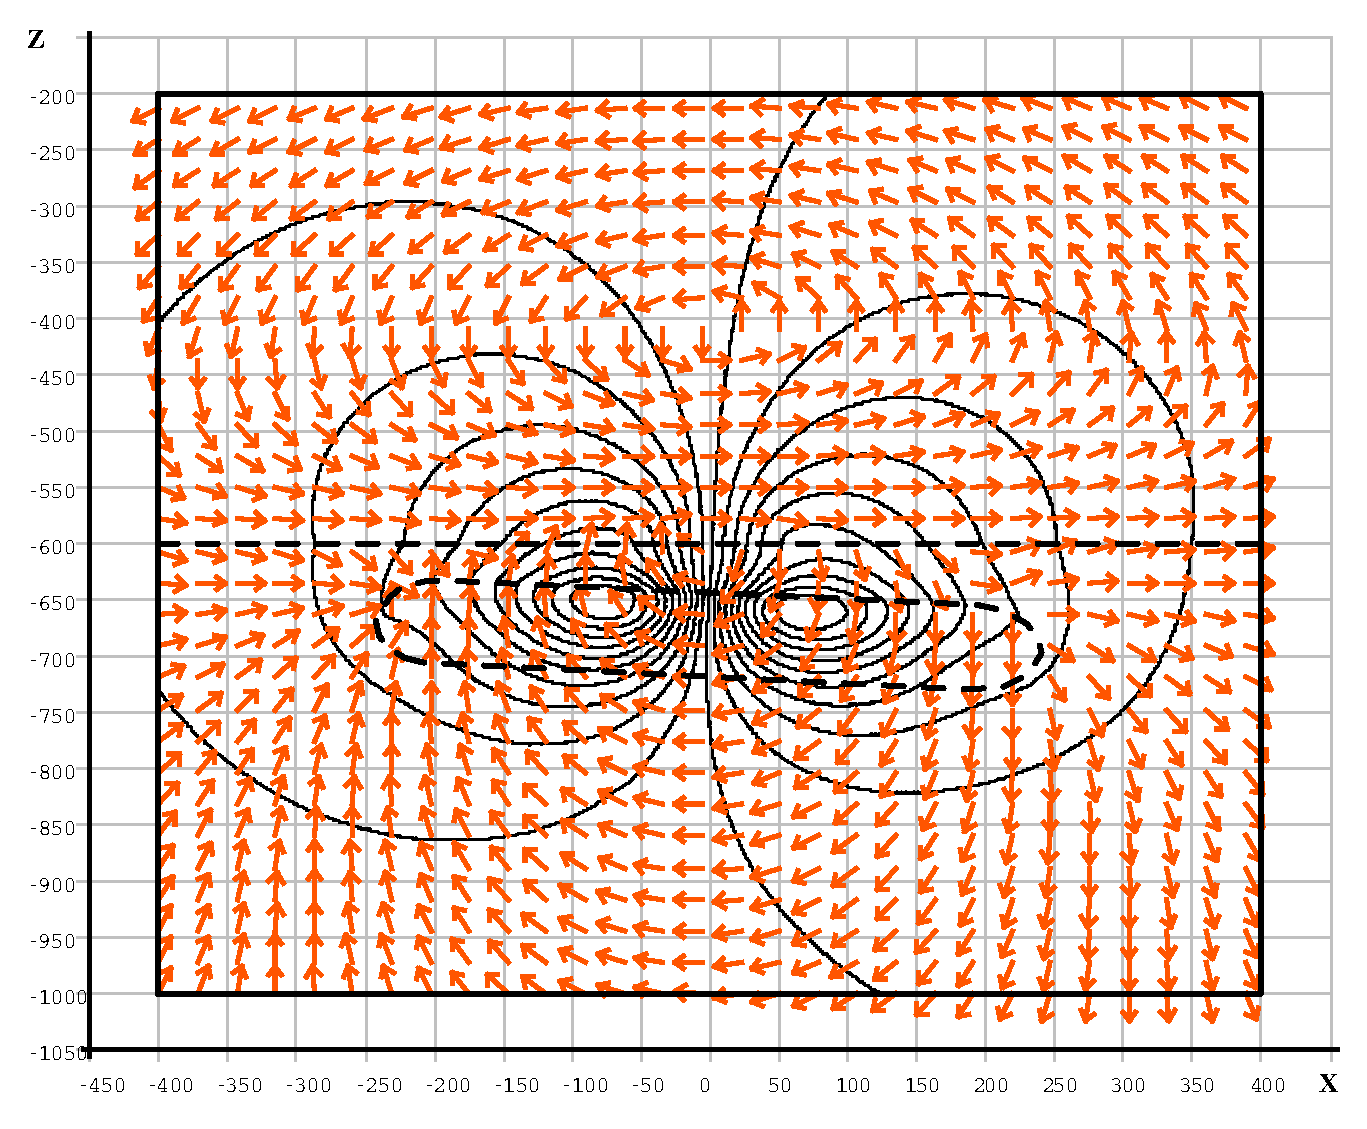
\includegraphics[scale=0.36]{research-3/fields/images/0/0_yes_y=0_vec.eps}\label{fig:res3:0_vec_b}}
	\caption{векторы $(\Re(\mathbf{E}_x), \Re{\mathbf{E}_z})^T$, изолинии $\Re(\mathbf{E}_y)$ при $l_2=0$}
	\label{fig:res3:0_vec}
\end{figure}

%\end{spacing}

На рисунках \ref{fig:res3:0_EzR_a} и \ref{fig:res3:0_EzR_b} показано графическое представление напряжённости электрического поля $\mathbf{E}$ при $l_2=0$ в сечении $z=-601$~м для объекта с $\sigma=10^{-2}$~См/м и для объекта с $\sigma=10^{2}$~См/м соответственно.

\begin{figure}[H]
	\centering
	\subfloat[][]{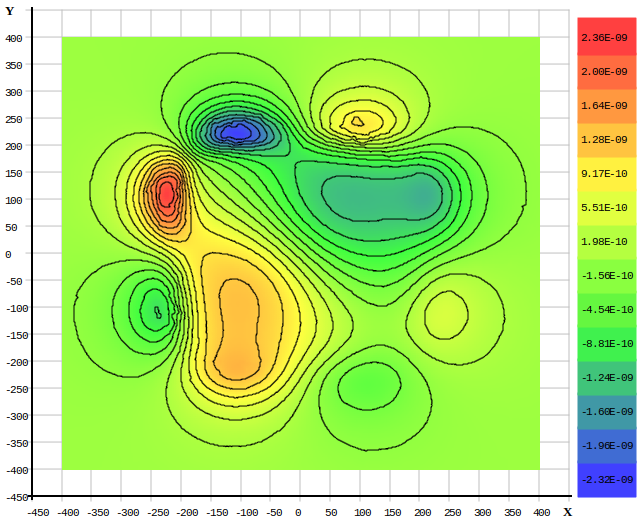
\includegraphics[scale=0.36]{research-3/fields/images/0/0_no_z=-601_EzR.eps}\label{fig:res3:0_EzR_a}}
	\text{~~}
	\subfloat[][]{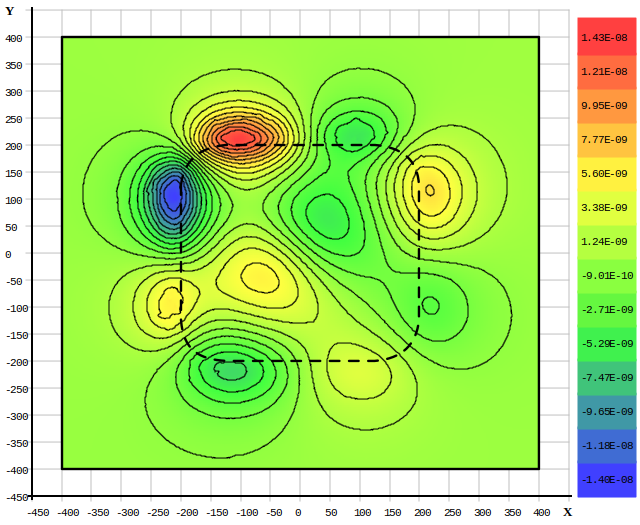
\includegraphics[scale=0.36]{research-3/fields/images/0/0_yes_z=-601_EzR.eps}\label{fig:res3:0_EzR_b}}
	\caption{$\Re(\mathbf{E}_z)$ при $l_2=0$}
	\label{fig:res3:0_EzR}
\end{figure}

На рисунках \ref{fig:res3:100_EyR}-\ref{fig:res3:100_vec} показано графическое представление напряжённости электрического поля $\mathbf{E}$ при $l_2=-100$ в сечении $y=0$, на рисунках \ref{fig:res3:100_EyR_a} и \ref{fig:res3:100_vec_a} -- для объекта с $\sigma=10^{-2}$~См/м, на рисунках \ref{fig:res3:100_EyR_b} и \ref{fig:res3:100_vec_b} -- для объекта с $\sigma=10^{2}$~См/м.

\begin{figure}[H]
	\centering
	\subfloat[][]{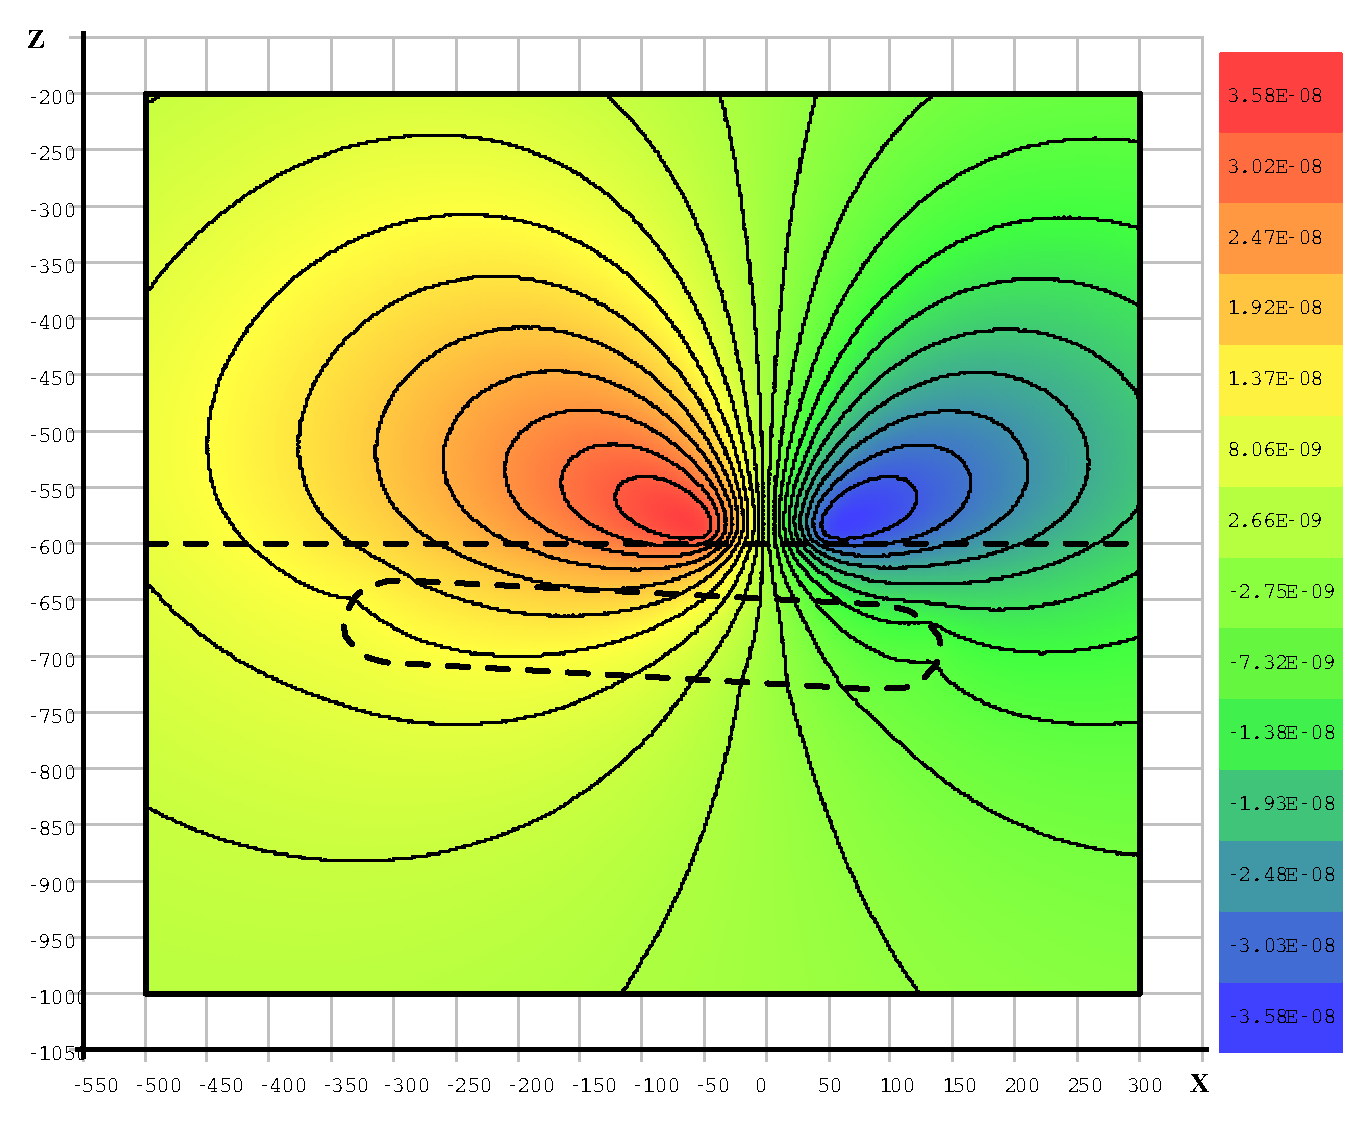
\includegraphics[scale=0.36]{research-3/fields/images/100/100_no_y=0_EyR.eps}\label{fig:res3:100_EyR_a}}
	\text{~~}
	\subfloat[][]{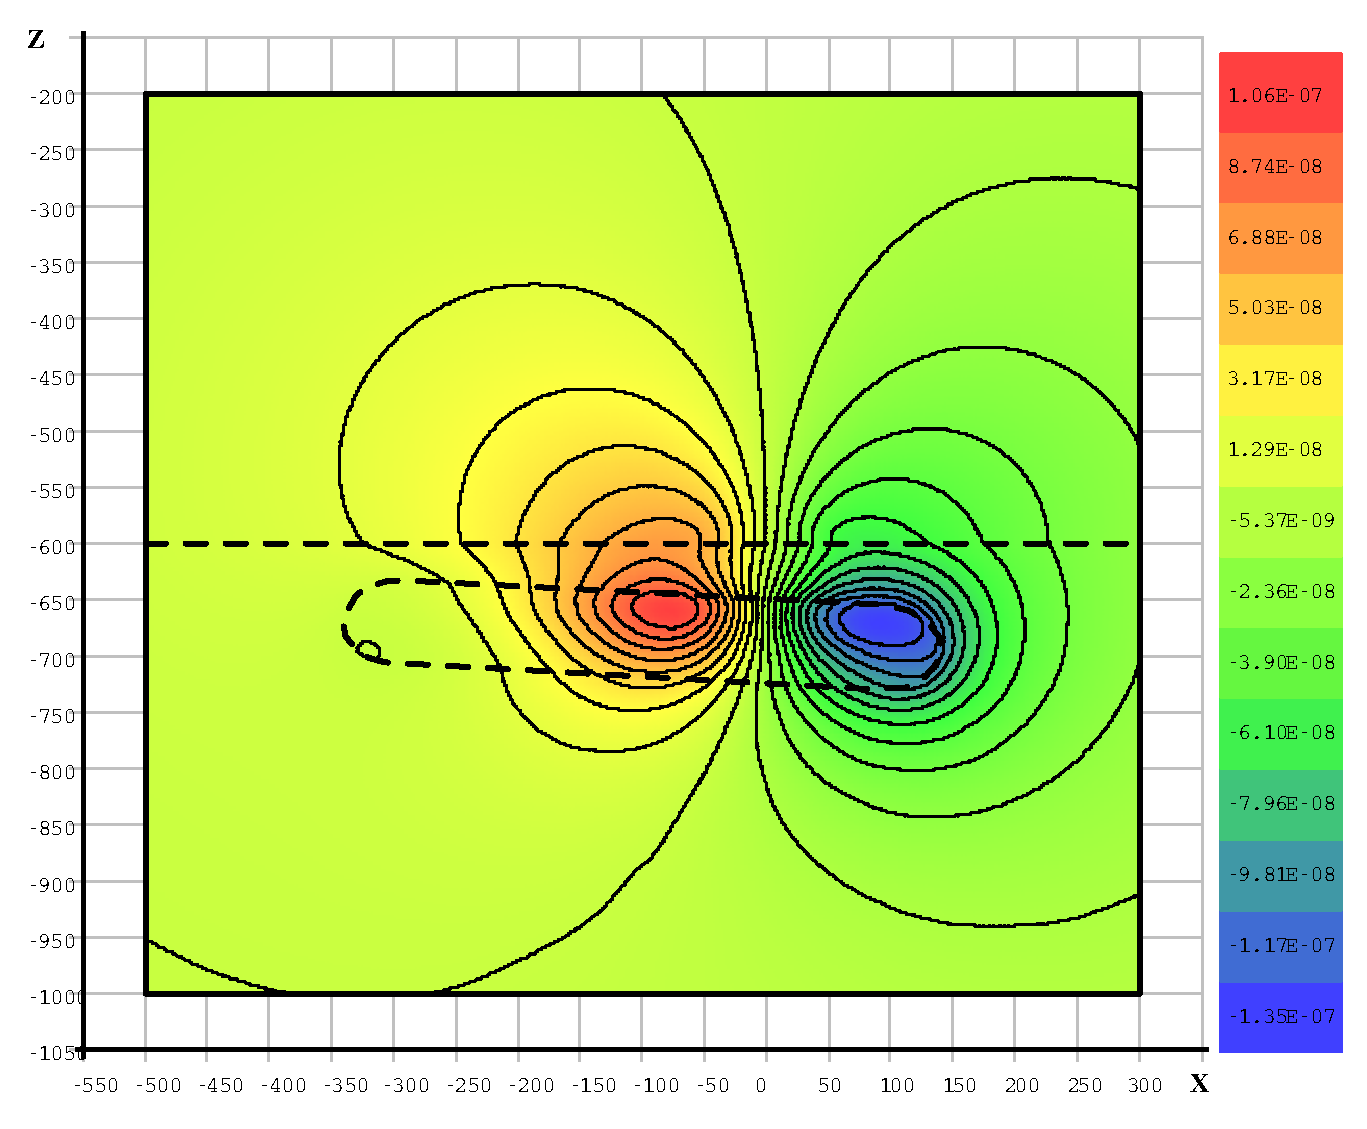
\includegraphics[scale=0.36]{research-3/fields/images/100/100_yes_y=0_EyR.eps}\label{fig:res3:100_EyR_b}}
	\caption{$\Re(\mathbf{E}_y)$ при $l_2=-100$}
	\label{fig:res3:100_EyR}
\end{figure}

\begin{figure}[H]
	\centering
	\subfloat[][]{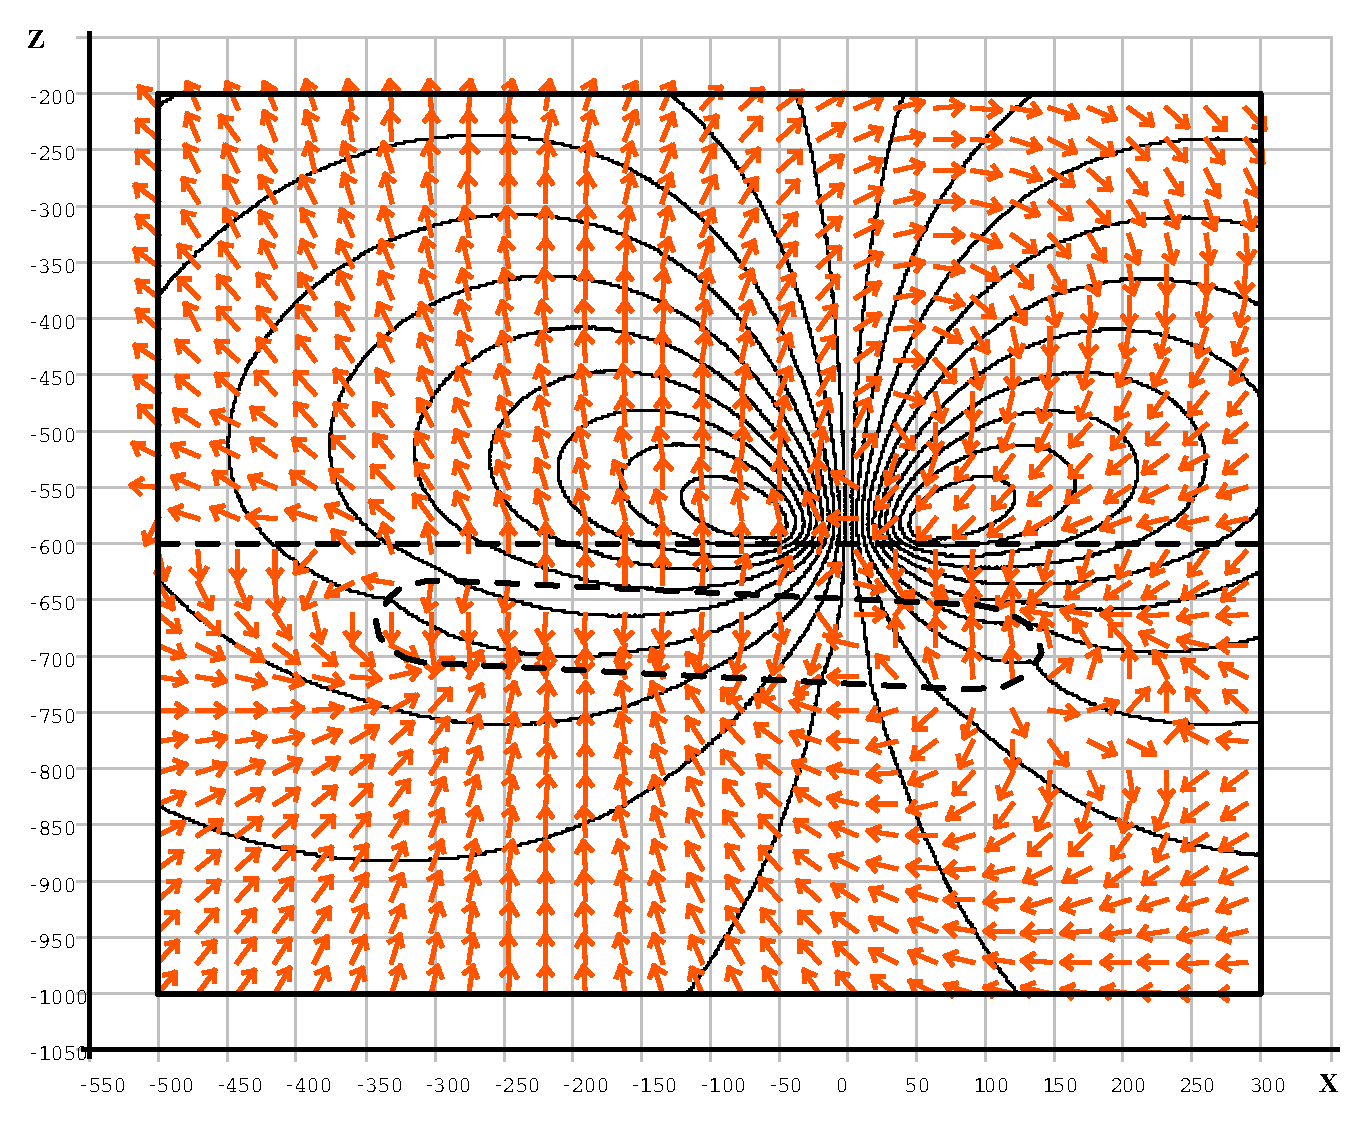
\includegraphics[scale=0.36]{research-3/fields/images/100/100_no_y=0_vec.eps}\label{fig:res3:100_vec_a}}
	\text{~~}
	\subfloat[][]{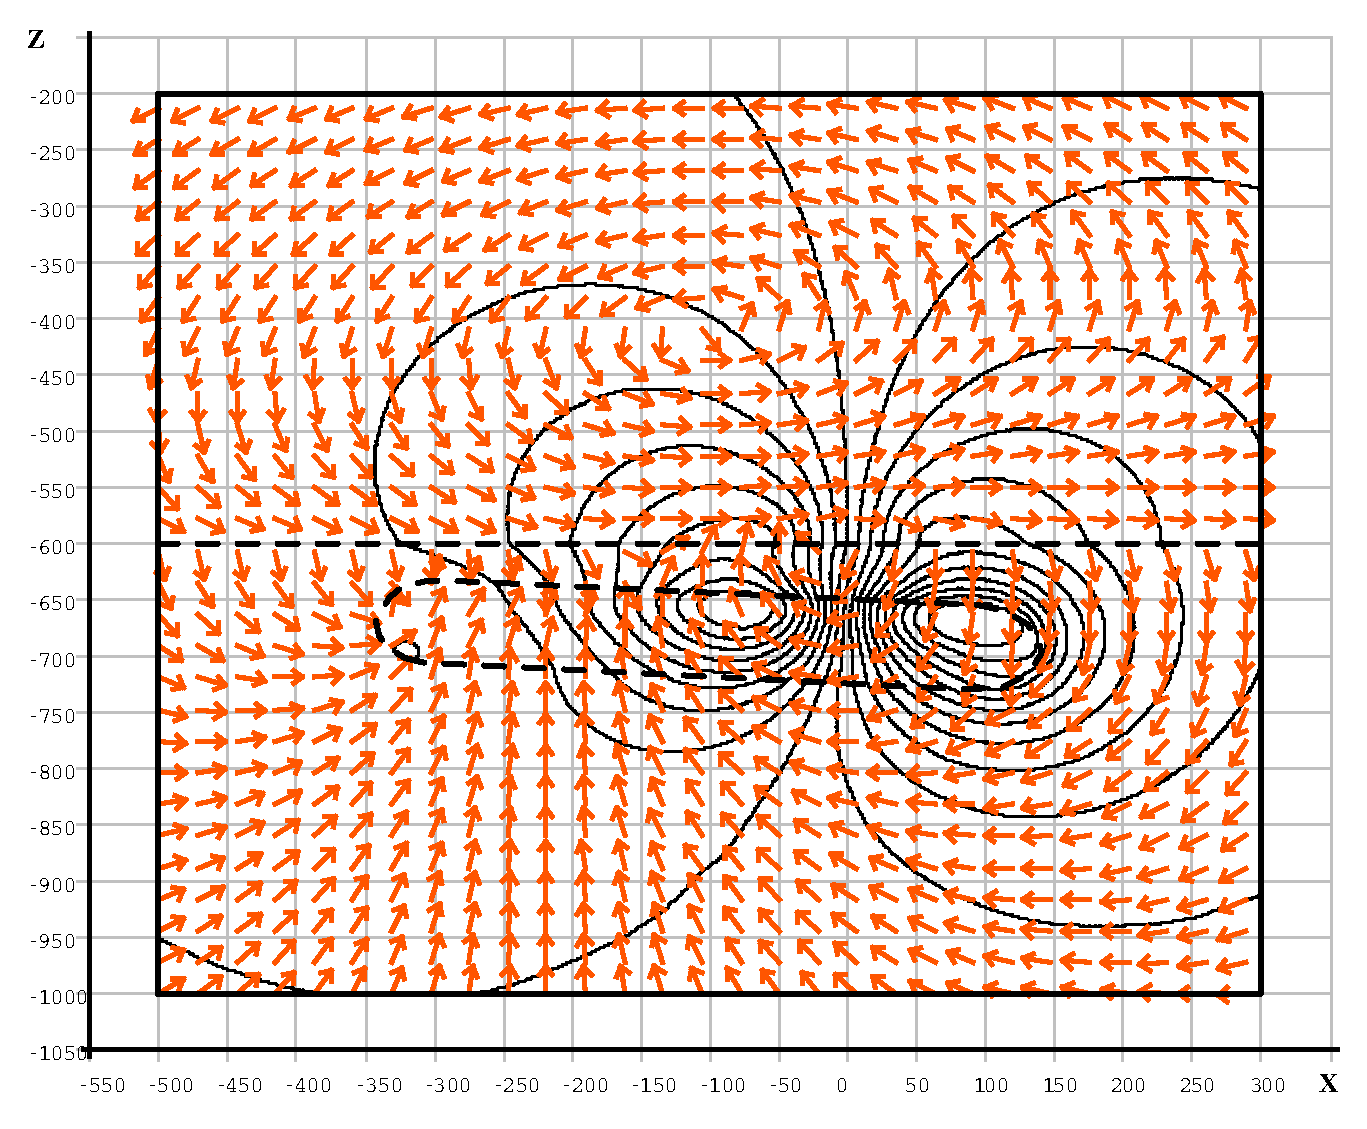
\includegraphics[scale=0.36]{research-3/fields/images/100/100_yes_y=0_vec.eps}\label{fig:res3:100_vec_b}}
	\caption{векторы $(\Re(\mathbf{E}_x), \Re{\mathbf{E}_z})^T$, изолинии $\Re(\mathbf{E}_y)$ при $l_2=-100$}
	\label{fig:res3:100_vec}
\end{figure}

На рисунках \ref{fig:res3:100_EzR_a} и \ref{fig:res3:100_EzR_b} показано графическое представление напряжённости электрического поля $\mathbf{E}$ при $l_2=-100$ в сечении $z=-601$~м для объекта с $\sigma=10^{-2}$~См/м и для объекта с $\sigma=10^{2}$~См/м соответственно.

\begin{figure}[H]
	\centering
	\subfloat[][]{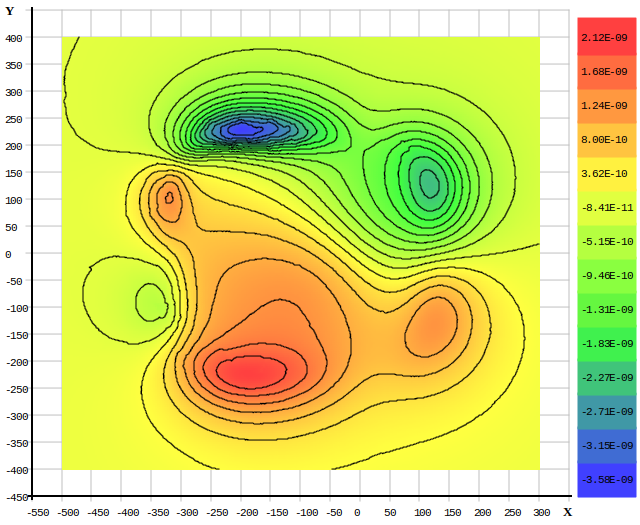
\includegraphics[scale=0.36]{research-3/fields/images/100/100_no_z=-601_EzR.eps}\label{fig:res3:100_EzR_a}}
	\text{~~}
	\subfloat[][]{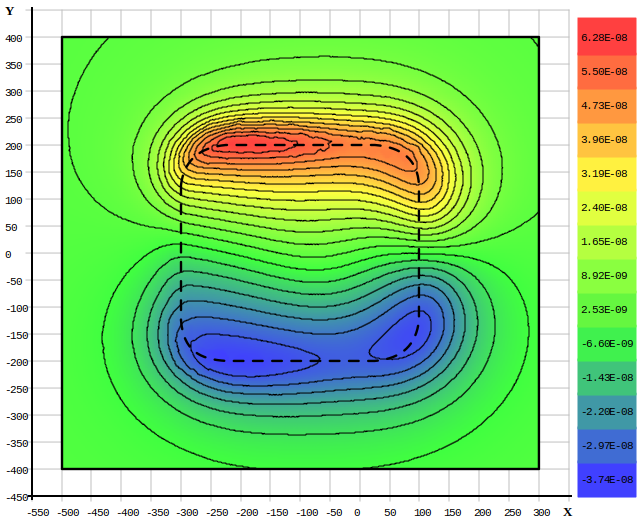
\includegraphics[scale=0.36]{research-3/fields/images/100/100_yes_z=-601_EzR.eps}\label{fig:res3:100_EzR_b}}
	\caption{$\Re(\mathbf{E}_z)$ при $l_2=-100$}
	\label{fig:res3:100_EzR}
\end{figure}

На рисунках \ref{fig:res3:200_EyR}-\ref{fig:res3:200_vec} показано графическое представление напряжённости электрического поля $\mathbf{E}$ при $l_2=-200$ в сечении $y=0$, на рисунках \ref{fig:res3:200_EyR_a} и \ref{fig:res3:200_vec_a} -- для объекта с $\sigma=10^{-2}$~См/м, на рисунках \ref{fig:res3:200_EyR_b} и \ref{fig:res3:200_vec_b} -- для объекта с $\sigma=10^{2}$~См/м.

\begin{figure}[H]
	\centering
	\subfloat[][]{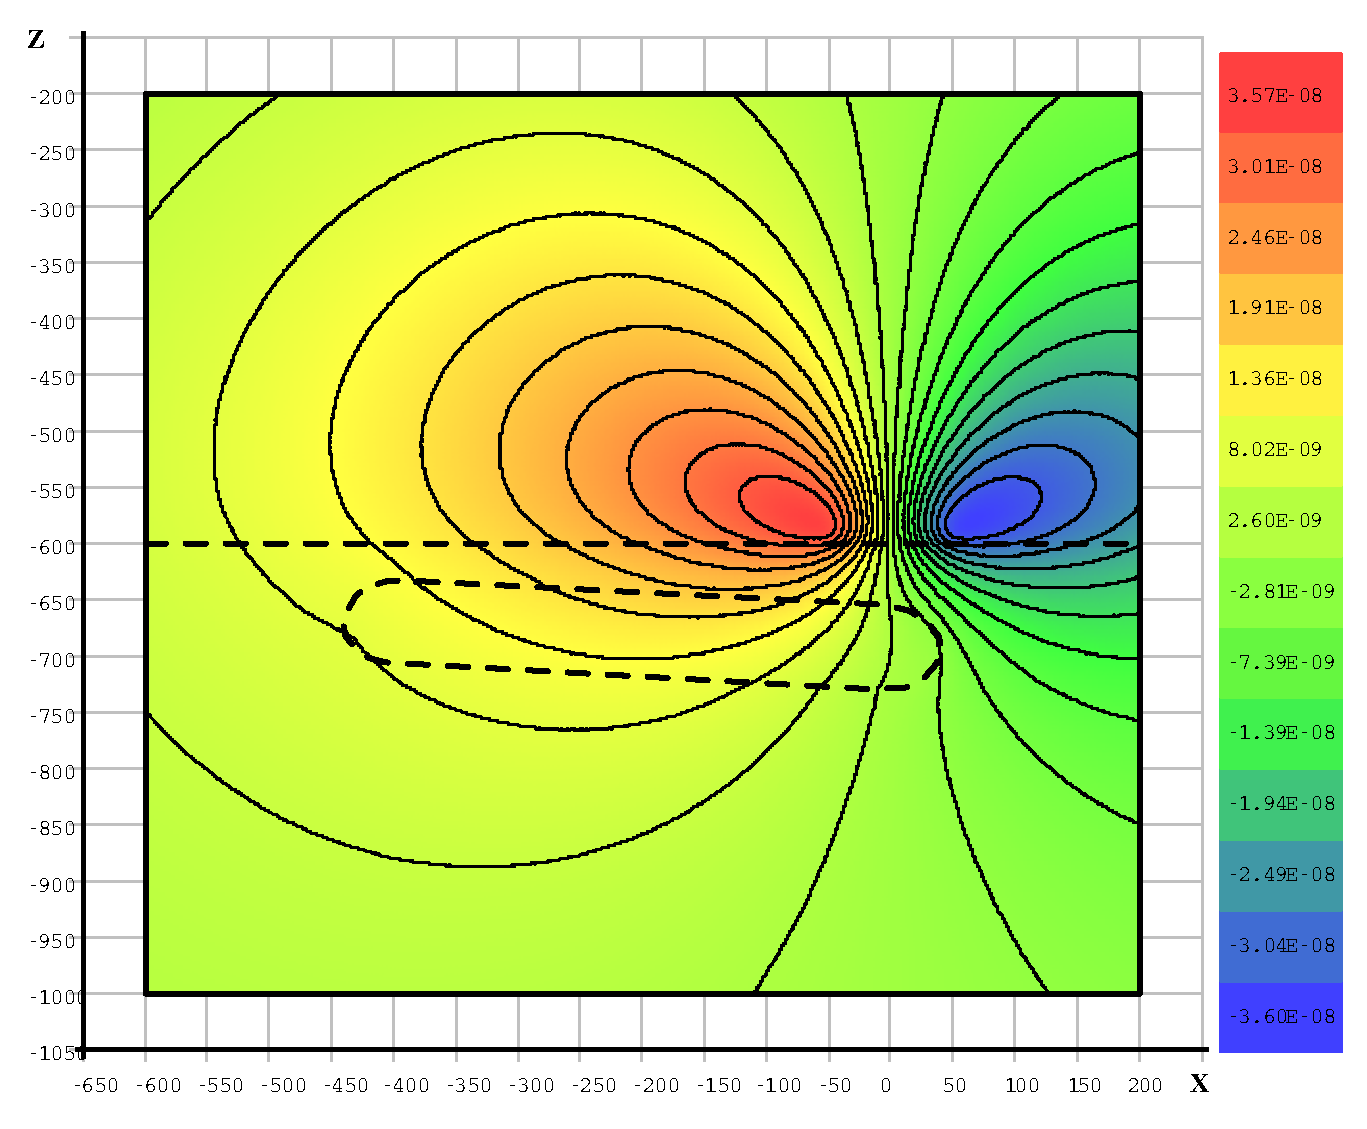
\includegraphics[scale=0.36]{research-3/fields/images/200/200_no_y=0_EyR.eps}\label{fig:res3:200_EyR_a}}
	\text{~~}
	\subfloat[][]{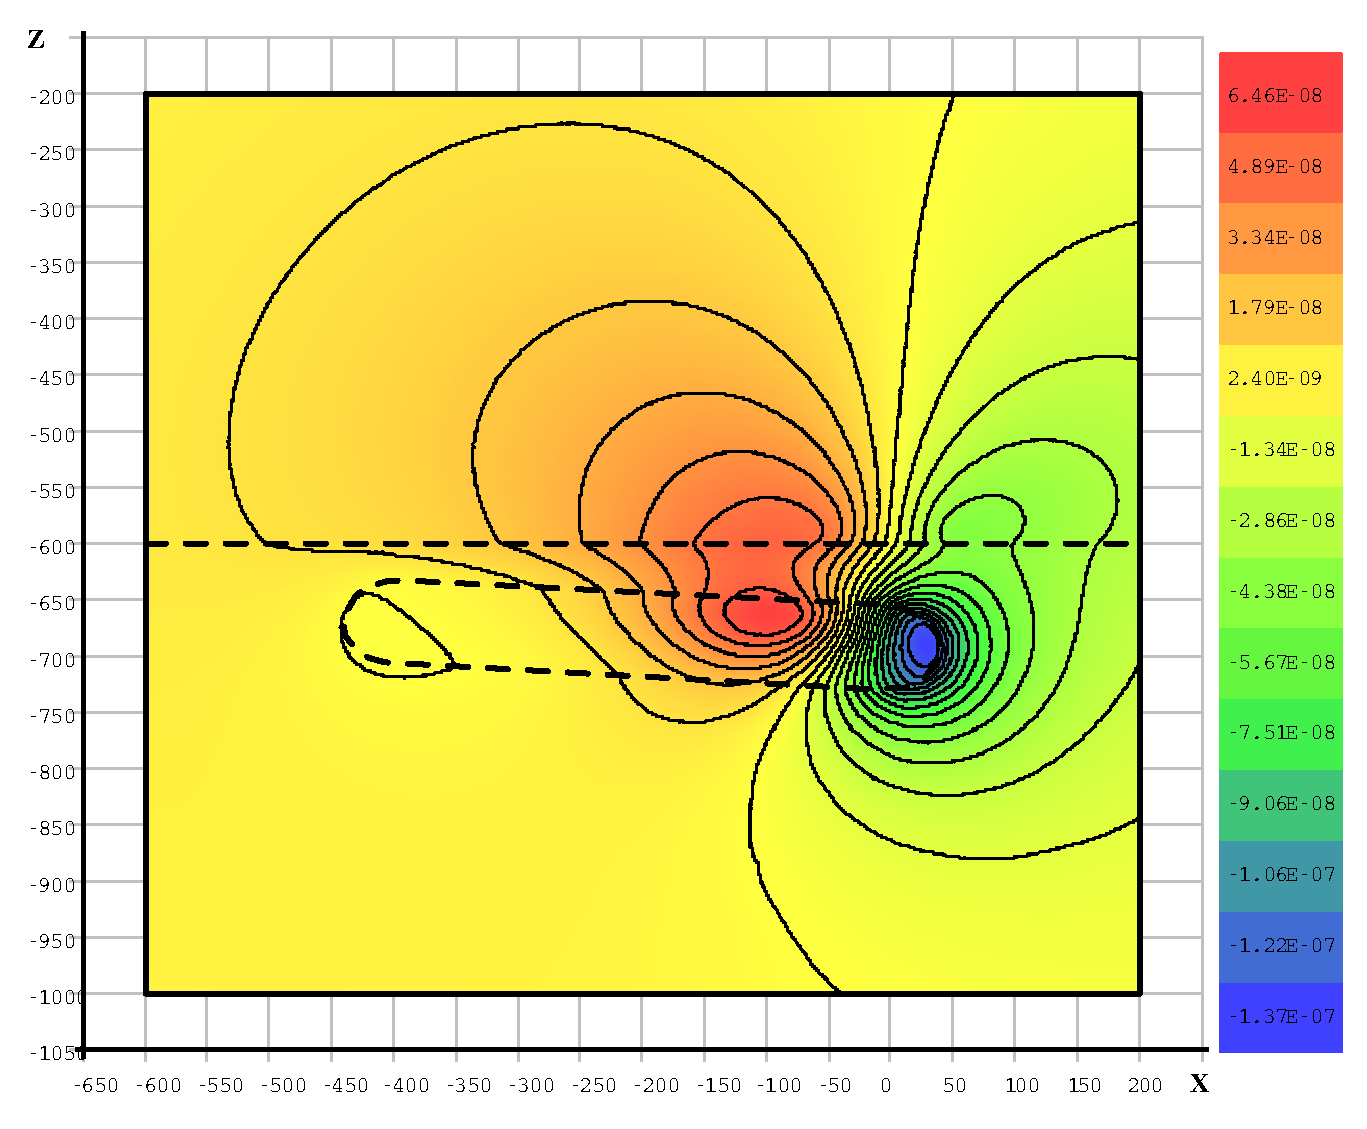
\includegraphics[scale=0.36]{research-3/fields/images/200/200_yes_y=0_EyR.eps}\label{fig:res3:200_EyR_b}}
	\caption{$\Re(\mathbf{E}_y)$ при $l_2=-200$}
	\label{fig:res3:200_EyR}
\end{figure}

\begin{figure}[H]
	\centering
	\subfloat[][]{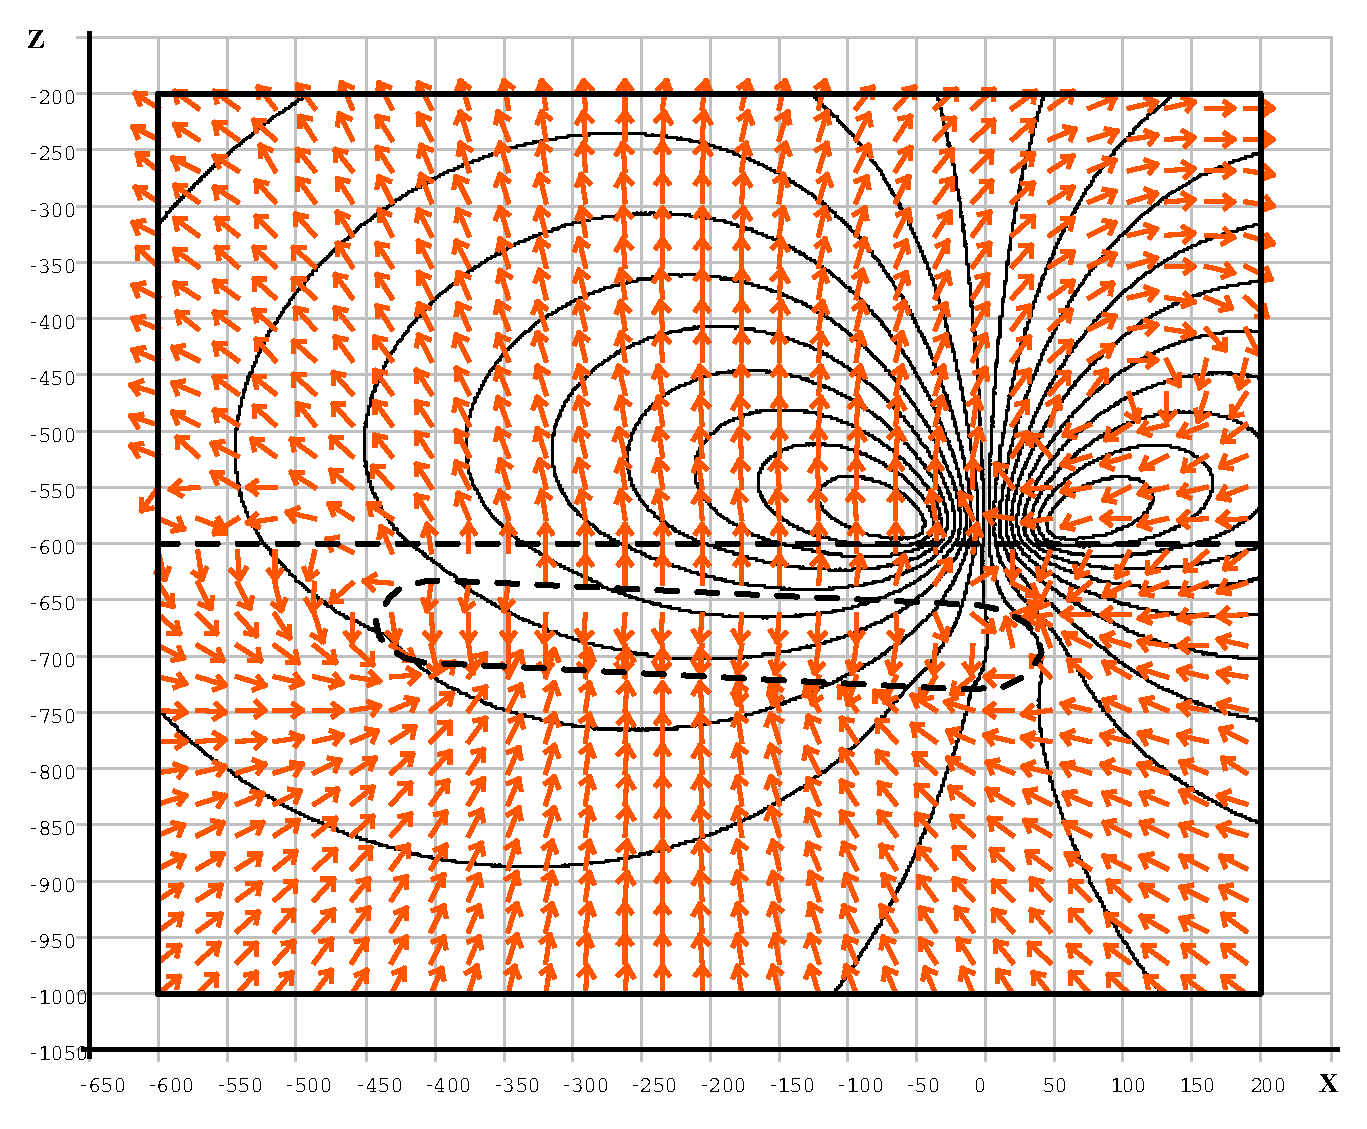
\includegraphics[scale=0.36]{research-3/fields/images/200/200_no_y=0_vec.eps}\label{fig:res3:200_vec_a}}
	\text{~~}
	\subfloat[][]{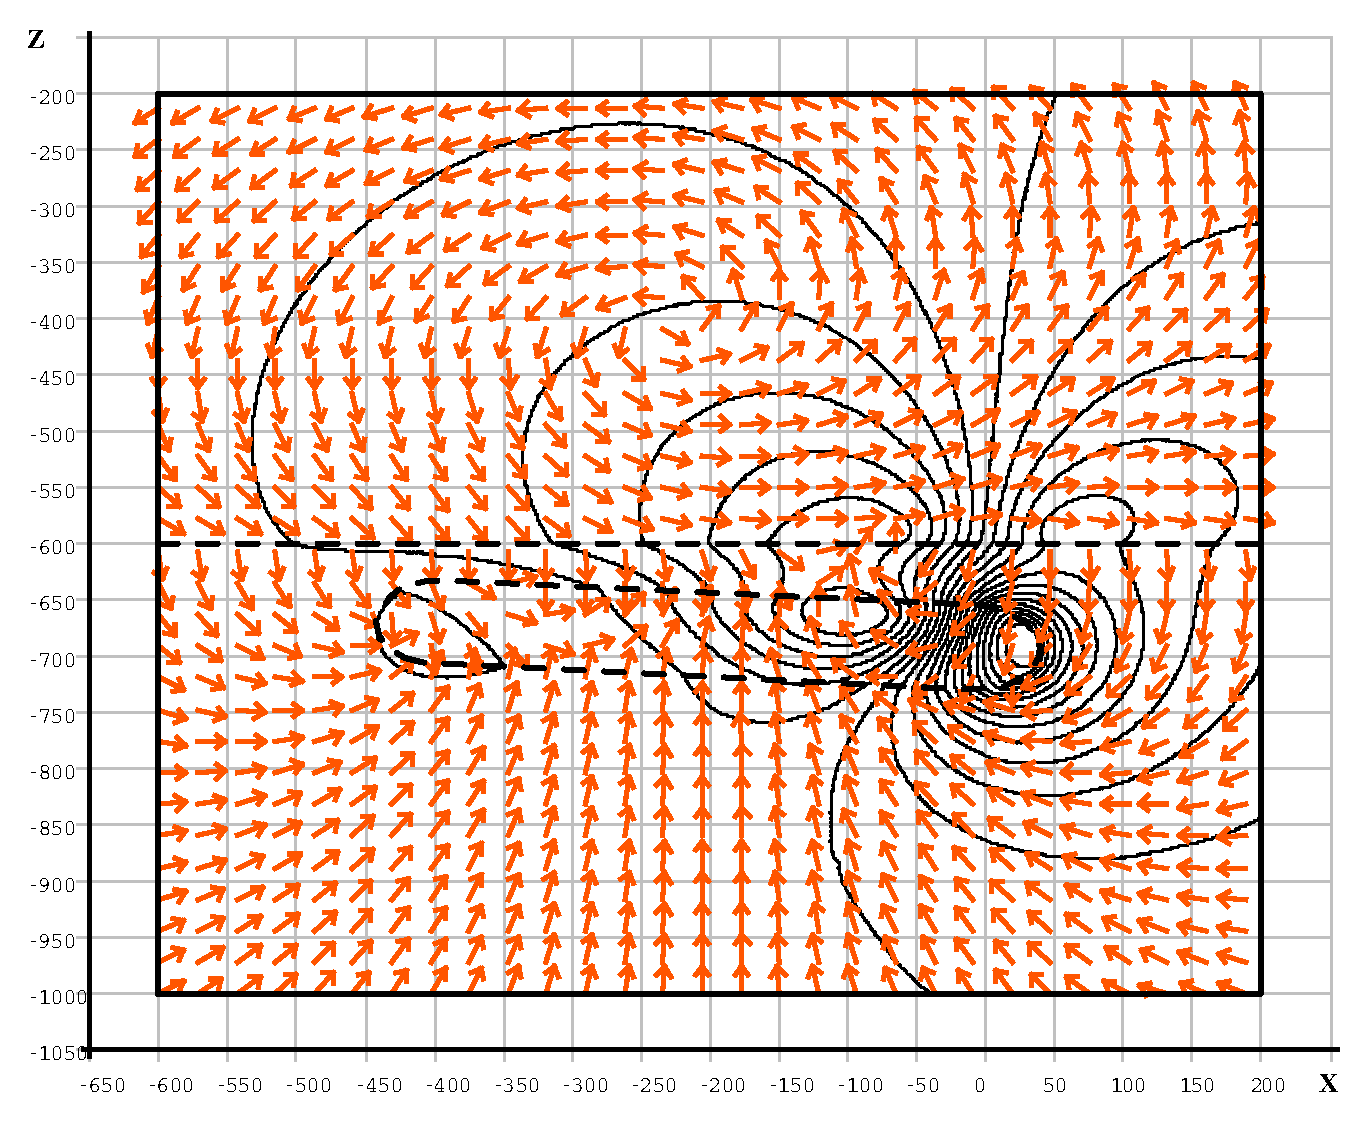
\includegraphics[scale=0.36]{research-3/fields/images/200/200_yes_y=0_vec.eps}\label{fig:res3:200_vec_b}}
	\caption{векторы $(\Re(\mathbf{E}_x), \Re{\mathbf{E}_z})^T$, изолинии $\Re(\mathbf{E}_y)$ при $l_2=-200$}
	\label{fig:res3:200_vec}
\end{figure}

На рисунках \ref{fig:res3:200_EzR_a} и \ref{fig:res3:200_EzR_b} показано графическое представление напряжённости электрического поля $\mathbf{E}$ при $l_2=-200$ в сечении $z=-601$~м для объекта с $\sigma=10^{-2}$~См/м и для объекта с $\sigma=10^{2}$~См/м соответственно.

\begin{figure}[H]
	\centering
	\subfloat[][]{\includegraphics[scale=0.36]{research-3/fields/images/200/200_no_z=-601_EzR.eps}\label{fig:res3:200_EzR_a}}
	\text{~~}
	\subfloat[][]{\includegraphics[scale=0.36]{research-3/fields/images/200/200_yes_z=-601_EzR.eps}\label{fig:res3:200_EzR_b}}
	\caption{$\Re(\mathbf{E}_z)$ при $l_2=-200$}
	\label{fig:res3:200_EzR}
\end{figure}

На рисунках \ref{fig:res3:300_EyR}-\ref{fig:res3:300_vec} показано графическое представление напряжённости электрического поля $\mathbf{E}$ при $l_2=-300$ в сечении $y=0$, на рисунках \ref{fig:res3:300_EyR_a} и \ref{fig:res3:300_vec_a} -- для объекта с $\sigma=10^{-2}$~См/м, на рисунках \ref{fig:res3:300_EyR_b} и \ref{fig:res3:300_vec_b} -- для объекта с $\sigma=10^{2}$~См/м.

\begin{figure}[H]
	\centering
	\subfloat[][]{\includegraphics[scale=0.36]{research-3/fields/images/300/300_no_y=0_EyR.eps}\label{fig:res3:300_EyR_a}}
	\text{~~}
	\subfloat[][]{\includegraphics[scale=0.36]{research-3/fields/images/300/300_yes_y=0_EyR.eps}\label{fig:res3:300_EyR_b}}
	\caption{$\Re(\mathbf{E}_y)$ при $l_2=-300$}
	\label{fig:res3:300_EyR}
\end{figure}

На рисунках \ref{fig:res3:300_EzR_a} и \ref{fig:res3:300_EzR_b} показано графическое представление напряжённости электрического поля $\mathbf{E}$ при $l_2=-300$ в сечении $z=-601$~м для объекта с $\sigma=10^{-2}$~См/м и для объекта с $\sigma=10^{2}$~См/м соответственно.

\begin{figure}[H]
	\centering
	\subfloat[][]{\includegraphics[scale=0.36]{research-3/fields/images/300/300_no_y=0_vec.eps}\label{fig:res3:300_vec_a}}
	\text{~~}
	\subfloat[][]{\includegraphics[scale=0.36]{research-3/fields/images/300/300_yes_y=0_vec.eps}\label{fig:res3:300_vec_b}}
	\caption{векторы $(\Re(\mathbf{E}_x), \Re{\mathbf{E}_z})^T$, изолинии $\Re(\mathbf{E}_y)$ при $l_2=-300$}
	\label{fig:res3:300_vec}
\end{figure}

\begin{figure}[H]
	\centering
	\subfloat[][]{\includegraphics[scale=0.36]{research-3/fields/images/300/300_no_z=-601_EzR.eps}\label{fig:res3:300_EzR_a}}
	\text{~~}
	\subfloat[][]{\includegraphics[scale=0.36]{research-3/fields/images/300/300_yes_z=-601_EzR.eps}\label{fig:res3:300_EzR_b}}
	\caption{$\Re(\mathbf{E}_z)$ при $l_2=-300$}
	\label{fig:res3:300_EzR}
\end{figure}


Результаты моделирования показывают, что проводящий объект хорошо <<виден>> и на некотором расстоянии от морского дна, а непроводящий -- только вблизи поверхности или при некотором заглублении приёмника в грунт, причём наибольший отклик на источник электромагнитного возмущения для непроводящего объекта наблюдается в том случае, когда этот источник расположен с некоторым смещением от центра симметрии объекта.

% =============================================================================

\clearpage
\section{Описание программного комплекса}
\labelname{4}\label{sec:program_description}
Разработанный программный комплекс ориентирован на решение задач, представимых в виде уравнения Гельмгольца, векторным методом конечных элементов. Комплекс написан на языке C++~\citep{cpp_2003} и может использовать стороннюю библиотеку Intel® MKL~\citep{intel_mkl} и распараллеливание с помощью OpenMP~\citep{openmp}, однако это не является обязательным -- достаточно любого компилятора C++, поддерживающего стандарт C++03 и новее. Программный комплекс не имеет жёсткой привязки к архитектуре процессора и операционной системе.

Этапы пре- и постпроцессинга выполняются сторонними программами. Построение конечноэлементной сетки выполняется с помощью пакета Gmsh~\citep{gmsh_article}. Регулярные тетраэдральные сетки могут быть построены с помощью пакета TetMeshGen~\citep{tet_mesh_gen}. Результаты работы программного комплекса выводятся в формате пакета Tecplot~\citep{tecplot}. В двумерном и одномерных случаях этот формат, помимо пакета Tecplot, может быть обработан в пакетах FEM~Draw~\citep{fem_draw} и gnuplot~\citep{gnuplot} соответственно.

Входными данными для программного комплекса являются аргументы командной строки, в которых задаются режим работы и расположение основных конфигурационных файлов; сами конфигурационные файлы, в которых задаются настройки программного комплекса, описания физических областей и PML-слоя; файл сетки в формате MSH ASCII file format~\citep{gmsh_doc}. Выходными данными для программного комплекса являются файлы в формате пакета Tecplot, а также файл с результатами решения СЛАУ. Параметры выходных данных задаются в основном конфигурационном файле.

\subsection{Формат конфигурационных файлов}
Конфигурационные файлы представляют собой файлы настроек в формате \CodeFont{ini}~\citep{ini_format}. Данный формат имеет простую структуру, поэтому легко обрабатывается программно и имеет понятный для чтения и редактирования человеком вид. Рассмотрим пример синтаксиса файлов подобного типа:

\vspace{-0.8cm}
\begin{singlespace}
\begin{footnotesize}
\begin{minted}{ini}
; Commentary
[Section]
parameter1 = value1
parameter2 = value2

[Section.Subsection]
parameter3 = value3
\end{minted}
\end{footnotesize}
\end{singlespace}
\vspace{-0.2cm}

\noindent В рассматриваемом примере \CodeFont{Commentary} -- комментарий; \CodeFont{Section} -- название секции, некоторая заранее определённая строка; \CodeFont{Subsection} -- название подсекции, используется как уникальный идентификатор подсекции, отличающий её от других подсекций той же секции; \CodeFont{parameterX} -- название параметра, строка из множества допустимых параметров для данной секции; \CodeFont{valueX} -- значение соответствующего параметра, тип значения определяется соответствующим параметром.

Подробные примеры конфигурационных файлов с пояснениями приведены в приложении \nameref{app:config_example}.

\subsection{Аргументы командной строки и переменные окружения}
В зависимости от режима работы программного комплекса список аргументов командной строки может оказаться различным.

\textbf{Режим решения.} Наиболее часто используемый режим, в процессе работы которого производится чтение исходных данных и решение задачи, после чего результат решения обрабатывается постпроцессором. Опции командной строки, доступные в таком режиме:

\CodeFont{programname [-nosolve|-continue] [-nopost] [config.ini]}

\noindent где \CodeFont{programname} -- имя программы; \CodeFont{-nosolve} -- ключ, по которому не будет проводиться процедура решения СЛАУ, вместо этого веса решения будут восстановлены из файла, указанного в основном конфигурационном файле; \CodeFont{-continue} -- ключ, по которому начальные веса будут взяты из файла, указанного в основном конфигурационном файле; \CodeFont{-nopost} -- ключ, отключающий постпроцессор; \CodeFont{config.ini} -- имя основного конфигурационного файла (по умолчанию -- <<config.ini>>).

\textbf{Режим сравнения.} Режим, в котором последовательное решение двух задач, а затем производится сравнение полученных решений в заданной подобласти $\Omega'$ в норме $\mathbb{L}^{2}(\Omega')$. Опции командной строки, доступные в таком режиме:

\CodeFont{programname -diff [-nosolve|-continue] [-nopost] master.ini [-nosolve|-continue] [-nopost] slave.ini diff.ini}

\noindent где \CodeFont{master.ini} -- имя конфигурационного файла для первичной задачи, сетка которой будет использоваться для численного интегрирования; \CodeFont{slave.ini} -- имя конфигурационного файла для вторичной задачи; \CodeFont{diff.ini} -- имя конфигурационного файла сравнения решений; остальные параметры идентичны таковым в режиме решения.

\textbf{Режим сравнения на идентичных сетках.} Режим, аналогичный предыдущему, с той лишь разницей, что сетки обеих задач должны быть геометрически идентичными в подобласти для сравнения $\Omega'$. За счёт такого ограничения сравнение решений выполняется значительно быстрее. Опции командной строки, доступные в таком режиме:

\CodeFont{programname -diff\_simple [-nosolve|-continue] [-nopost] master.ini [-nosolve|-continue] [-nopost] slave.ini diff.ini}

\noindent все параметры идентичны параметрам в режиме сравнения.

Для тонкой настройки работы программы доступны также некоторые переменные окружения:
\begin{itemize}
	\item \CodeFont{NO\_PROGRESS} -- отключает вывод прогресса текущей операции (по умолчанию прогресс показывается);
	\item \CodeFont{OMP\_NUM\_THREADS=N} -- устанавливает количество доступных потоков в подпрограммах, использующих OpenMP (по умолчанию -- 1);
	\item \CodeFont{MKL\_NUM\_THREADS=N} -- устанавливает количество доступных потоков в подпрограммах, использующих Intel® MKL (по умолчанию -- 1);
	\item \CodeFont{GMRES\_M=N} -- устанавливает глубину метода для решателей на базе GMRES (по умолчанию -- 5).
\end{itemize}

%\subsubsection{Формат основного конфигурационного файла}
%Основной конфигурационный файл может содержать восемь типов секций: секция \CodeFont{VFEM}, в которой содержатся основные настройки для решения задачи; секция \CodeFont{Boundary}, в которой определяются глобальные параметры неоднородных краевых условий~(\ref{eq:bound1}); секции вида \CodeFont{Boundary.NUM}, в которых определяются параметры неоднородных краевых условий~(\ref{eq:bound1}) для конкретной двумерной физической области с номером \CodeFont{NUM} (границы трехмерных областей); секция \CodeFont{Right}, в которой определяются глобальные параметры неоднородных правых частей $i \omega \mathbf{J}$; секции вида \CodeFont{Right.NUM}, в которых определяются параметры неоднородных правых частей $i \omega \mathbf{J}$ для конкретной трехмерной физической области с номером \CodeFont{NUM}; секция \CodeFont{Analytical}, в которой определяются глобальные параметры аналитического решения; секции вида \CodeFont{Analytical.NUM}, в которых определяются параметры аналитического решения для конкретной трехмерной физической области с номером \CodeFont{NUM}; секции вида \CodeFont{Postprocessing.NUM}, в которых определяются параметры постпроцессора, где \CodeFont{NUM} -- положительное число, являющееся идентификатором постпроцессора. В случае отсутствия необходимости задавать неоднородные краевые условия, неоднородную правую часть, аналитическое решение или постпроцессор, секции \CodeFont{Boundary[.NUM]}, \CodeFont{Right[.NUM]}, \CodeFont{Analytical[.NUM]} или \CodeFont{Postprocessing[.NUM]} соответственно могут быть не указаны. Упрощенный пример конфигурационного файла:
%
%\vspace{-0.8cm}
%\begin{singlespace}
%\begin{small}
%\begin{verbatim}
%[VFEM]
%basis_order = 1
%basis_type = 2
%tet_integration_order = 4
%tr_integration_order = 5
%eps_slae = 1e-10
%eps_slae_bound = 1e-15
%v_cycle_enabled = yes
%gamma_v_cycle_0 = 0.1
%gamma_v_cycle_full = 0.5
%gamma_v_cycle_ker = 0.1
%max_iter = 15000
%max_iter_v_cycle_local = 100
%solver_name = "COCG<LLT>"
%solver_name_bound = "COCG<LLT>"
%solver_name_v_cycle_full = "GMRES<LLT>"
%solver_name_v_cycle_ker = "GMRES<LLT>"
%filename_mesh = "mesh.msh"
%filename_phys = "phys.ini"
%filename_pml = "config_pml.ini"
%filename_slae = "solution.txt"
%jit_type = inline
%
%[Boundary]
%enabled = yes
%x = 0.0
%y = 0.0
%z = 0.0
%
%[Boundary.42]
%x = 0
%y = exp(- (0.5 - x) * (0.5 - x) - (0.5 - z) * (0.5 - z))
%z = exp(- (0.5 - x) * (0.5 - x) - (0.5 - y) * (0.5 - y))
%
%[Right]
%enabled = yes
%x = exp(-0.5 * x) / mu + k2 * exp(- (0.5 - x))
%y = exp(-0.5 * y) / mu + k2 * exp(- (0.5 - x))
%z = exp(-0.5 * z) / mu + k2 * exp(- (0.5 - z))
%
%[Right.42]
%x = 0.0
%y = 0.0
%z = 0.0
%
%[Analytical]
%enabled = yes
%x = exp(- (0.5 - y) * (0.5 - y) - (0.5 - z) * (0.5 - z))
%y = exp(- (0.5 - x) * (0.5 - x) - (0.5 - z) * (0.5 - z))
%z = exp(- (0.5 - x) * (0.5 - x) - (0.5 - y) * (0.5 - y))
%
%[Analytical.42]
%x = 0.0
%y = 0.0
%z = 0.0
%
%[Postprocessing.1]
%type = 3d
%filename = "area_3layers_inc_loop_pml.plt"
%timestamp = yes
%
%[Postprocessing.2]
%type = 2d
%filename = "area_3layers_inc_loop_pml_y=0.dat"
%timestamp = yes
%slice_var_name = Y
%slice_var_value = 0.0
%var1_name = X
%var1_from = -700
%var1_to = 700
%var1_num = 70
%var2_name = Z
%var2_from = -700
%var2_to = 700
%var2_num = 70
%
%[Postprocessing.3]
%type = 1d
%filename = "z=-100.dat"
%timestamp = yes
%line_var1_name = Y
%line_var1_value = 0.0
%line_var2_name = Z
%line_var2_value = -100
%var_name = X
%var_from = -600
%var_to = 600
%var_num = 70
%\end{verbatim}
%\end{small}
%\end{singlespace}
%\vspace{-0.25cm}
%
%\noindent где \CodeFont{basis\_order} -- порядок базисных функций, 1 или 2; \CodeFont{basis\_type} -- тип базисных функций, 1 или 2; \CodeFont{tet\_integration\_order} -- порядок интегрирования на тетраэдральных элементах, от 2 до 14 включительно;  \CodeFont{tr\_integration\_order} -- порядок интегрирования на треугольных элементах, от 2 до 29 включительно; \CodeFont{eps\_slae} -- точность решения основной СЛАУ~(\ref{eq:form_29}); \CodeFont{eps\_slae\_bound} -- точность решения СЛАУ неоднородных краевых условий~(\ref{eq:bound_mnk}); \CodeFont{v\_cycle\_enabled} -- использовать двухуровневый решатель или нет;  \CodeFont{gamma\_v\_cycle\_0} -- точность нахождения начального приближения в двухуровневом решателе; \CodeFont{gamma\_v\_cycle\_full} -- точность решения СЛАУ на полном пространстве в двухуровневом решателе; \CodeFont{gamma\_v\_cycle\_ker} -- точность решения СЛАУ на пространстве ядра в двухуровневом решателе; \CodeFont{max\_iter} -- максимальное количество итераций для не двухуровневых решателей; \CodeFont{max\_iter\_v\_cycle\_local} -- максимальное количество итераций при решении СЛАУ на полном пространстве и пространстве ядра в двухуровневом решателе; \CodeFont{solver\_name}, \CodeFont{solver\_name\_bound}, \CodeFont{solver\_name\_v\_cycle\_full} и \CodeFont{solver\_name\_v\_cycle\_ker} -- названия решателей для решения основной СЛАУ, СЛАУ неоднородных краевых условий, СЛАУ на полном пространстве в двухуровневом решателе и СЛАУ на пространстве ядра в двухуровневом решателе соответственно; \CodeFont{filename\_mesh}, \CodeFont{filename\_phys}, \CodeFont{filename\_pml} и \CodeFont{filename\_slae} -- пути к файлам сетки, конфигурации физических областей, конфигурации PML-слоя и файлу для хранения весов решения соответственно; \CodeFont{jit\_type}
%
%
%
%\subsubsection{Формат конфигурационного файла физических областей}
%Конфигурационный файл физических областей может содержать четыре типа секций: секция \CodeFont{Global}, в которой определяются глобальные физические параметры; секции вида \CodeFont{Phys3D.NUM}, в которых определяются параметры среды для конкретной трехмерной физической области с номером \CodeFont{NUM}; секции вида \CodeFont{Phys2D.NUM}, в которых определяются параметры среды для конкретной двумерной физической области с номером \CodeFont{NUM} (границы трехмерных областей); секции вида \CodeFont{Phys1D.NUM}, в которых определяются параметры среды для конкретной одномерной физической области с номером \CodeFont{NUM} (ребра для описания петли, являющейся источником поля). Упрощенный пример конфигурационного файла:
%
%\vspace{-0.8cm}
%\begin{singlespace}
%\begin{small}
%\begin{verbatim}
%[Global]
%frequency = 10
%mu = 1
%eps = 1
%sigma = 0.2
%
%[Phys3D.1]
%sigma = 3.3
%
%[Phys2D.1]
%parent = 1
%boundary = 1
%
%[Phys1D.1]
%parent = 1
%current = 1.0
%\end{verbatim}
%\end{small}
%\end{singlespace}
%\vspace{-0.25cm}
%
%\noindent где \CodeFont{frequency} -- частота источника поля $\nu = \frac{\omega}{2 \pi}$; \CodeFont{mu} -- относительная магнитная проницаемость $\mu_{r}$; \CodeFont{eps} -- относительная диэлектрическая проницаемость $\varepsilon_{r}$; \CodeFont{sigma} -- электрическая проводимость; \CodeFont{parent} -- номер трехмерной физической области, частью которой является текущая двумерная или одномерная область; \CodeFont{boundary} -- тип краевого условия, 1 и 2 для (\ref{eq:bound1}) и (\ref{eq:bound2}) соответственно; \CodeFont{current} -- электрический ток $I$.
%
%\subsubsection{Формат конфигурационного файла PML-слоя}
%
%Конфигурационный файл PML-слоя содержит в себе два типа секций -- секция \CodeFont{PML}, в которой определяются глобальные параметры PML-слоя в задаче, а также секции вида \CodeFont{PML.NUM}, в которых определяются параметры PML-слоя для конкретной физической области с номером \CodeFont{NUM}. Упрощенный пример конфигурационного файла:
%
%\vspace{-0.8cm}
%\begin{singlespace}
%\begin{small}
%\begin{verbatim}
%[PML]
%x0 = -600
%x1 = 600
%y0 = -600
%y1 = 600
%z0 = -600
%z1 = 600
%chi_real = 1
%chi_imag = 0
%m = 3
%width = 100
%
%[PML.21]
%chi_real = 2
%chi_imag = 3
%m = 3
%width = 100
%\end{verbatim}
%\end{small}
%\end{singlespace}
%\vspace{-0.25cm}
%
%\noindent где \CodeFont{x0}, \CodeFont{x1}, \CodeFont{y0}, \CodeFont{y1}, \CodeFont{z0}, \CodeFont{z1} -- границы внутренней области без PML-слоя, определяются автоматически, если их не указать явно; \CodeFont{chi\_real}, \CodeFont{chi\_imag} -- вещественная и мнимая части коэффициента комплексного растяжения $\chi$~(\ref{eq:pml_s}), по умолчанию растяжение не производится; \CodeFont{m} -- степенной параметр $m$~(\ref{eq:pml_s}), по умолчанию $m=3$; \CodeFont{width} -- толщина PML-слоя $\delta_k$, по умолчанию равная $100$~м.
%
%\subsubsection{Формат конфигурационного файла сравнения решений}
%
%Конфигурационный файл сравнения решений содержит секции одного типа -- \CodeFont{Area.NUM}, где \CodeFont{NUM} -- положительное число, являющееся идентификатором области. Области могут быть двух типов: included и excluded, это означает, что область будет включена в подобласть $\Omega'$ или исключена из нее соответственно. Упрощенный пример конфигурационного файла:
%
%\vspace{-0.8cm}
%\begin{singlespace}
%\begin{small}
%\begin{verbatim}
%[Area.1]
%type = included
%x0 = -500
%x1 = 500
%y0 = -500
%y1 = 500
%z0 = -500
%z1 = 500
%
%[Area.2]
%type = excluded
%x0 = -180
%x1 = 180
%y0 = -180
%y1 = 180
%z0 = -180
%z1 = 180
%\end{verbatim}
%\end{small}
%\end{singlespace}
%\vspace{-0.25cm}
%
%\noindent где \CodeFont{type} -- тип области; \CodeFont{x0}, \CodeFont{x1}, \CodeFont{y0}, \CodeFont{y1}, \CodeFont{z0}, \CodeFont{z1} -- границы области.

% =============================================================================

\clearpage
\phantomsection
\section*{Заключение}
\addcontentsline{toc}{section}{Заключение}
В работе были реализованы алгоритмы на базе векторного метода конечных элементов. Эти алгоритмы были положены в основу программного комплекса, который позволяет моделировать электромагнитные поля в областях разнообразной структуры. С помощью этого программного комплекса были решены модельные задачи морской геоэлектрики на низких частотах, проведены исследования возможности сокращения области моделирования без внесения дополнительных погрешностей.

На основании исследований были сделаны выводы, что расчёты, в которых в область моделирования не включается воздух, допустимы только при расположении источника электромагнитного поля на большой глубине, иначе, из-за неправильного учёта физических процессов, происходящих в воздухе, полученное решение будет неверным.

Применение PML-слоя позволило получить достаточно точные решения, однако его применение не привело к резкому уменьшению размерности систем уравнений и, как следствие, к уменьшению времени решения. Было выдвинуто предположение, что увеличить эффективность применения PML-слоя можно с помощью применения неконформных методов, в которых конечноэлементная сетка может содержать геометрические носители разного типа: тетраэдры и параллелепипеды.

Расчёты на модельной задаче с проводящим и непроводящим объектами показали, что проводящий объект хорошо <<виден>> на некотором расстоянии от морского дна, а непроводящий -- только вблизи дна или при небольшом заглублении приёмника в грунт. Наибольший отклик на источник электромагнитного возмущения для непроводящего объекта наблюдался в том случае, когда источник располагался со смещением от центра симметрии объекта.

% =============================================================================

\clearpage
\addcontentsline{toc}{section}{Список литературы}

%\begin{spacing}{1.1}

\begin{thebibliography}{10}
% 1
\bibitem{shurina} 
Шурина, Э.П. Морская геоэлектрика -- задачи и перспективы / Э.П.~Шурина, М.И.~Эпов, А.В.~Мариенко // Тез. докл. всеросс. науч.-техн. конф. <<Научное и техническое обеспечение исследования и освоения шельфа Северного Ледовитого океана>>. -- 2010. -- 9-13~августа. -- С.~7-12.
% 2
\bibitem{gabrielsen} 
Gabrielsen, P.T. 3D CSEM for Hydrocarbon Exploration in the Barents Sea / P.T.~Gabrielsen, D.V.~Shantsev, S.~Fanavoll // 5th Saint Petersburg International Conference \& Exhibition -- Geosciences: Making the most of the Earth’s resources. -- 2012. -- 2-5~April. -- Pp.~1-5.
% 3
\bibitem{anderson}
Anderson, C. An integrated approach to marine electromagnetic surveying using a towed streamer and source / C. Anderson, J. Mattsson // First Break. -- May~2010. -- Vol.~28, Iss.~5. -- Pp.~71-75.
% 4
\bibitem{conf_nti_2015}
Жигалов, П.С. Влияние слоя воздуха в задачах морской геоэлектрики / П.С.~Жигалов, Б.В.~Рак // Наука. Технологии. Инновации. : сб. науч. трудов -- Новосибирск : Изд-во НГТУ, 2015 -- 01-05~декабря -- Часть 2 -- С.~56-57.
% 5
\bibitem{mur}
Mur G. Absorbing boundary conditions for the finite-difference approximation of the time-domain electromagnetic-field equations // Electromagnetic Compatibility, IEEE Transactions on. -- 1981. -- No.~4. -- Pp.~377-382.
% 6
\bibitem{berenger}
Berenger, J.P. A perfectly matched layer for the absorption of electromagnetic waves / J.P. Berenger // Journal of computation physics. -- 1994 -- No.~114. -- Pp.~185-200.
% 7
\bibitem{wiik_dehoop_ursin}
Wiik, T. A Discontinuous Galerkin Method for Modelling Marine Controlled Source Electromagnetic Data / T.~Wiik, M.V.~De Hoop, B.~Ursin // Proceedings of the Project Review, Geo-Mathematical Imaging Group, Purdue University, West Lafayette, IN. -- 2013 -- Vol.~1 -- P.~75-102.
% 8
\bibitem{balandin_vfem}
Баландин, М.Ю. Векторный метод конечных элементов : Учеб. пособие / М.Ю.~Баландин, Э.П.~Шурина. -- Новосибирск : Изд-во НГТУ, 2001. -- 69~с.
% 9
\bibitem{monk}
Monk P. Finite element methods for Maxwell's equations. / P.~Monk -- Oxford University Press, 2003.
% 10
\bibitem{conf_english_2015}
Zhigalov, P. Analysis of the Source-Receiver Systems in Marine Geoelectric Problems / P.~Zhigalov // Progress Through Innovation : Тез. городск. науч.-практ. конф. аспирантов и магистрантов. -- Новосибирск : 2015. -- 2~апреля. -- С.~30-31.
% 11
\bibitem{conf_mnsk_academ_2015}
Жигалов, П.С. Анализ систем источник-приемник в задачах морской геоэлектрики / П.С.~Жигалов // МНСК-2015 : матер. 53 междунар. научн. студенч. конф. -- Новосибирск : 2015 -- 11-17~апреля -- Математика -- С.~216.
% 12
\bibitem{conf_achm_2015}
Шурина, Э.П. Математическое моделирование электромагнитного поля для задачи морской геоэлектрики / Э.П.~Шурина, Б.В.~Рак, П.С.~Жигалов // Аналитические и численные методы моделирования естественно-научных и социальных проблем : сб. ст. X междунар. науч.-техн. конф. -- Пенза : Изд-во ПГУ, 2015. -- 28-30~октября. -- С.~131-137.
% 13
\bibitem{conf_radio_day_2015}
Жигалов, П.С. Идеально согласованные слои / П.С.~Жигалов, Б.В.~Рак // Обработка информации и математическое моделирование. Росс. науч.-техн. конф. : матер. конф. -- Новосибирск : 2015 -- С.~106-114.
% 14
\bibitem{epov}
Эпов, М.И. Параллельные конечноэлементные вычислительные схемы в задачах геоэлектрики / М.И.~Эпов, Э.П.~Шурина, Д.А.~Архипов // Вычислительные технологии. -- 2013. -- Том~18, №2. -- С.~94-112.
% 15
\bibitem{schwarzbach}
Schwarzbach C. Stability of finite element solutions to Maxwell's equations in frequency domain. / C.~Schwarzbach -- 2009.
% 16
\bibitem{hiptmair}
Hiptmair R. Multigrid method for Maxwell's equations / R.~Hiptmair // SIAM Journal on Numerical Analysis. -- 1998. -- Vol.~36. -- No.~1. -- Pp.~204-225.
% 17
\bibitem{nedelec1980}
Nédélec J.C. Mixed finite elements in $\mathbb{R}$3 / J.C.~Nédélec // Numerische Mathematik. -- 1980. -- Vol.~35. -- No.~3. -- Pp.~315-341.
% 18
\bibitem{nedelec1986}
Nédélec J.C. A new family of mixed finite elements in $\mathbb{R}$3 / J.C.~Nédélec // Numerische Mathematik. -- 1986. -- Vol.~50. -- No.~1. -- Pp.~57-81.
% 19
\bibitem{webb1993}
Webb J.P. Edge elements and what they can do for you / J.P.~Webb // Magnetics, IEEE Transactions on. -- 1993. -- Vol.~29. -- No.~2. -- Pp.~1460-1465.
% 20
\bibitem{balandin_slae}
Баландин М.Ю. Методы решения СЛАУ большой размерности: Учеб. пособие / М.Ю.~Баландин, Э.П.~Шурина. -- Новосибирск : Изд-во НГТУ, 2000. -- 70~с.
% 21
\bibitem{soloveychick}
Соловейчик, Ю.Г. Метод конечных элементов для решения скалярных и векторных задач : учеб. пособие / Ю.Г.~Соловейчик, М.Э.~Рояк, М.Г.~Персова. -- Новосибирск : Изд-во НГТУ, 2007. -- 896~с.
% 22
\bibitem{webb1999}
Webb, J.P. Hierarchal Vector Basis Functions of Arbitrary Order for Triangular and Tetrahedral Finite Elements / J.P.~Webb // IEEE transactions on antennas and propagation. -- 1999. -- Vol.~47. -- Pp.~1244-1253.
% 23
\bibitem{nechaev}
Nechaev, O.V. Multilevel iterative solver for the edge fem solution of the 3D Maxwell equation / O.V.~Nechaev, E.P.~Shurina, M.A.~Botchev // Computers and Mathematics with Applications. -- 2008. -- No.~55. -- Pp.~2346-2362.
% 24
\bibitem{mikhajlova}
Михайлова Е.И., Шурина Э.П. Математическое моделирование высокочастотного электромагнитного поля в волноводных устройствах / Е.И.~Михайлова, Э.П.~Шурина // Вестник НГУ. Серия: Математика, механика, информатика. -- 2013. -- Т.~13. -- №.~4. -- С.~102-118.
% 25
\bibitem{misovskih}
Мысовских И.П. Интерполяционные кубатурные формулы. -- Наука. Гл. ред. физ.-мат. лит., 1981.
% 26
\bibitem{zhang_integration}
Zhang L. et al. A set of symmetric quadrature rules on triangles and tetrahedra / L.~Zhang, T.~Cui, H.~Liu // J. Comput. Math. -- 2009. -- Vol.~27. -- No.~1. -- Pp.~89-96.
% 27
\bibitem{tet_integration}
Numerical Integration over the Tetrahedral Domain [Электронный ресурс]. -- Режим доступа: \href{https://web.archive.org/web/20140714140951/https://people.fh-landshut.de/~maurer/numeth/node148.html}{\url{https://people.fh-landshut.de/~maurer/numeth/node148.html}}.
% 28
\bibitem{tr_integration}
Numerical Integration over the Triangular Domain [Электронный ресурс]. -- Режим доступа: \href{https://web.archive.org/web/20140714120045/https://people.fh-landshut.de/~maurer/numeth/node147.html}{\url{https://people.fh-landshut.de/~maurer/numeth/node147.html}}.
% 29
\bibitem{shokin_multigrid}
Шокин Ю.И. Современные многосеточные методы. -- Часть II. Многоуровневые методы. Применение многомасштабных методов.: Учеб. пособие / Ю.И. Шокин, Э.П. Шурина, Н.Б. Иткина. -- Новосибирск : Изд-во НГТУ, 2012. -- 98~с.
% 30
\bibitem{solver_saad}
Saad Y. Iterative methods for sparse linear systems. / Y.~Saad -- Siam, 2003.
% 31
\bibitem{solver_iterative}
Van der Vorst H.A. Iterative Krylov methods for large linear systems. / H.A.~Van der Vorst -- Cambridge University Press, 2003. -- Vol.~13.
% 32
\bibitem{solver_templates}
Barrett R. et al. Templates for the solution of linear systems: building blocks for iterative methods. / R.~Barrett et~al. -- Siam, 1994. -- Vol.~43.
% 33
\bibitem{extra_elements1}
Solin P., Segeth K., Dolezel I. Higher-order finite element methods. / P.~Solin, K.~Segeth, I.~Dolezel -- CRC Press, 2003. -- 388~p.
% 34
\bibitem{extra_elements2}
Bergot M., Duruflé M. High-order optimal edge elements for pyramids, prisms and hexahedra / M.~Bergot, M.~Duruflé // Journal of Computational Physics. -- 2013. -- Vol.~232. -- No.~1. -- Pp.~189-213.
% 35
\bibitem{dg1}
Dosopoulos S., Zhao B., Lee J.F. Non-conformal and parallel discontinuous Galerkin time domain method for Maxwell’s equations: EM analysis of IC packages / S.~Dosopoulos, B.~Zhao, J.F.~Lee // Journal of Computational Physics. -- 2013. -- Vol.~238. -- Pp.~48-70.
% 36
\bibitem{dg2}
Perugia I., Schötzau D. The \textit{hp}-local discontinuous Galerkin method for low-frequency time-harmonic Maxwell equations / I.~Perugia, D.~Schötzau // Mathematics of Computation. -- 2003. -- Vol.~72. -- No.~243. -- Pp.~1179-1214.
% 37
\bibitem{dg3}
Dosopoulos S., Lee J.F. Interconnect and lumped elements modeling in interior penalty discontinuous Galerkin time-domain methods / S.~Dosopoulos, J.F.~Lee // Journal of Computational Physics. -- 2010. -- Vol.~229. -- No.~22. -- Pp.~8521-8536.
% 38
\bibitem{mortar1}
Christophe A. et al. An Overlapping Nonmatching Grid Mortar Element Method for Maxwell's Equations / A.~Christophe et al. // Magnetics, IEEE Transactions on. -- 2014. -- Vol.~50. -- Iss.~2. -- Pp.~409-412.
% 39
\bibitem{mortar2}
Gopalakrishnan J., Pasciak J.E. Multigrid for the mortar finite element method / J.~Gopalakrishnan, J.E.~Pasciak // SIAM Journal on Numerical Analysis. -- 2000. -- Vol.~37. -- No.~3. -- Pp.~1029-1052.
% 40
\bibitem{cpp_2003}
International organization for standardization, ISO/IEC 14882:2003: Programming languages: C++, 2nd ed. -- Geneva, Switzerland, 2003 -- 757~p.
% 41
\bibitem{intel_mkl}
Intel® Math Kernel Library (Intel® MKL) [Электронный ресурс]. -- Режим доступа: \href{https://software.intel.com/en-us/intel-mkl}{\url{https://software.intel.com/en-us/intel-mkl}}.
% 42
\bibitem{openmp}
OpenMP Application Programming Interface: Version~4.5 November~2015 -- OpenMP Architecture Review Board. -- 2015. -- 368~p.
% 43
\bibitem{gmsh_article}
Geuzaine C. Gmsh: a three-dimensional finite element mesh generator with built-in pre- and post-processing facilities / C.~Geuzaine J.F.~Remacle. // International Journal for Numerical Methods in Engineering -- 2009 -- Vol.~79 -- Iss.~11 -- Pp.~1309-1331
% 44
\bibitem{tet_mesh_gen}
TetMeshGen: A regular tetrahedral finite element mesh generator [Электронный ресурс]. -- Режим доступа: \href{https://github.com/AlienCowEatCake/tet_mesh_gen}{\url{https://github.com/AlienCowEatCake/tet_mesh_gen}}.
% 45
\bibitem{tecplot}
Tecplot 10 User’s Manual -- Amtec Engineering, Inc., Bellevue, Washington., 2003.
% 46
\bibitem{fem_draw}
FEM Draw: The software for visualization of scalar and vector fields [Электронный ресурс]. -- Режим доступа: \href{https://github.com/AlienCowEatCake/fem_draw}{\url{https://github.com/AlienCowEatCake/fem_draw}}.
% 47
\bibitem{gnuplot}
Williams T. gnuplot 5.0: An Interactive Plotting Program / T.~Williams, C.~Kelley -- 2016. -- 254~p.
% 48
\bibitem{gmsh_doc}
Gmsh Reference Manual [Электронный ресурс]. -- Режим доступа: \href{http://gmsh.info/doc/texinfo/gmsh.html}{\url{http://gmsh.info/doc/texinfo/gmsh.html}}.
% 49
\bibitem{ini_format}
.ini: Формат файла [Электронный ресурс]. -- Режим доступа: \href{https://ru.wikipedia.org/w/index.php?title=.ini&oldid=75247596}{\url{https://ru.wikipedia.org/wiki/.ini}}.

\end{thebibliography}

%\end{spacing}

% =============================================================================

\clearpage
\phantomsection
\section*{Приложение А. Примеры конфигурационных файлов}
\labelname{А}\label{app:config_example}
\addcontentsline{toc}{section}{Приложение А. Примеры конфигурационных файлов}

\subsectioncode{ini}{sources/configs/config.ini}{Пример основного конфигурационного файла}
\pagebreak
\subsectioncode{ini}{sources/configs/phys.ini}{Пример конфигурационного файла физических областей}
\subsectioncode{ini}{sources/configs/config_pml.ini}{Пример конфигурационного файла PML-слоя}
\subsectioncode{ini}{sources/configs/diff.ini}{Пример конфигурационного файла сравнения решений}

% =============================================================================

\clearpage
\phantomsection
\section*{Приложение Б. Интерфейсы основных классов программного комплекса}
\labelname{Б}\label{app:interfaces}
\addcontentsline{toc}{section}{Приложение Б. Интерфейсы основных классов программного комплекса}

\subsectioncodeauto{cpp}{sources/src}{vfem/vfem/vfem.h}
\subsectioncodeauto{cpp}{sources/src}{vfem/vfem/phys.h}
\subsectioncodeauto{cpp}{sources/src}{vfem/vfem/slae.h}
\subsectioncodeauto{cpp}{sources/src}{vfem/problems/problems.h}
\subsectioncodeauto{cpp}{sources/src}{vfem/elements/tetrahedron.h}
\pagebreak
\subsectioncodeauto{cpp}{sources/src}{vfem/elements/triangle.h}
\subsectioncodeauto{cpp}{sources/src}{vfem/elements/edge.h}
\subsectioncodeauto{cpp}{sources/src}{vfem/common/config.h}
\subsectioncode{cpp}{sources/src/vfem/common/evaluator_helmholtz.h}{Файл vfem/common/evaluator\_helmholtz.h}
\subsectioncodeauto{cpp}{sources/src}{vfem/common/common.h}

\subsectioncode{cpp}{sources/src/core/containers/fem/tetrahedron_basic.h}{Файл core/containers/fem/tetrahedron\_basic.h}
\subsectioncode{cpp}{sources/src/core/containers/fem/tetrahedron_basic_3d.h}{Файл core/containers/fem/tetrahedron\_basic\_3d.h}
\subsectioncode{cpp}{sources/src/core/containers/fem/triangle_basic.h}{Файл core/containers/fem/triangle\_basic.h}
\subsectioncode{cpp}{sources/src/core/containers/fem/triangle_basic_3d.h}{Файл core/containers/fem/triangle\_basic\_3d.h}

\subsectioncodeauto{cpp}{sources/src}{core/containers/tree/octree.h}

\subsectioncode{cpp}{sources/src/core/containers/geometry/edge_basic.h}{Файл core/containers/geometry/edge\_basic.h}
\subsectioncode{cpp}{sources/src/core/containers/geometry/face_triangle_basic.h}{Файл core/containers/geometry/face\_triangle\_basic.h}
\subsectioncode{cpp}{sources/src/core/containers/geometry/vector3_t.h}{Файл core/containers/geometry/vector3\_t.h}
\pagebreak
\subsectioncode{cpp}{sources/src/core/containers/geometry/point3_t.h}{Файл core/containers/geometry/point3\_t.h}

\subsectioncode{cpp}{sources/src/core/cubatures/tetrahedron_integration.h}{Файл core/cubatures/tetrahedron\_integration.h}
\subsectioncode{cpp}{sources/src/core/cubatures/triangle_integration.h}{Файл core/cubatures/triangle\_integration.h}

\subsectioncode{cpp}{sources/src/core/solvers/CSLR/preconditioners/preconditioner_interface.h}{Файл core/solvers/CSLR/preconditioners/preconditioner\_interface.h}
\subsectioncode{cpp}{sources/src/core/solvers/CSLR/symmetric/symmetric_solver_interface.h}{Файл core/solvers/CSLR/symmetric/symmetric\_solver\_interface.h}
\subsectioncode{cpp}{sources/src/core/solvers/CSLR/solvers_factory.h}{Файл core/solvers/CSLR/symmetric/solvers\_factory.h}

\subsectioncodeauto{cpp}{sources/src}{core/utils/inifile.h}

\subsectioncodeauto{cpp}{sources/src}{core/evaluator/evaluator.h}
\subsectioncode{cpp}{sources/src/core/evaluator/evaluator_operations.h}{Файл sources/src/core/evaluator/evaluator\_operations.h}
\subsectioncode{cpp}{sources/src/core/evaluator/evaluator_xyz.h}{Файл sources/src/core/evaluator/evaluator\_xyz.h}

% =============================================================================

\end{document}
